\documentclass[11pt,a4paper,oneside]{report}

\usepackage{soul}
\usepackage{tabularx}
\usepackage{longtable}
\usepackage{colortbl}
\usepackage{ltxtable}


\usepackage{tikz}
\usetikzlibrary{shapes,positioning,calc}
\definecolor{darkgreen}{rgb}{0,0.5,0}

% Schrift
\usepackage[utf8]{inputenc}
\usepackage{lmodern}
\usepackage{textcomp}

% UTF8-Zeichencode
\usepackage[utf8]{inputenc}

% Dokoument in deutsch
\usepackage{ngerman}

\definecolor{clBlue}{rgb}{.122,.286,.490}
\definecolor{clChapTxt}{rgb}{.090,.212,.365}
\newcommand{\parspace}{\setlength{\parskip}{10pt}}
% Zeilenabstand
\linespread{1.15}
\makeatletter
\renewcommand{\section}{\@startsection {section}{1}{\z@}%
                                   {-3.5ex \@plus -1ex \@minus -.2ex}%
                                   {2.3ex \@plus.2ex}%
                                   {\rmfamily\Large\bfseries\boldmath\color{clBlue}}}
\renewcommand{\subsection}{\@startsection{subsection}{2}{\z@}%
                                     {-3.25ex\@plus -1ex \@minus -.2ex}%
                                     {1.5ex \@plus .2ex}%
                                     {\rmfamily\large\bfseries\boldmath\color{clBlue}}}
\renewcommand{\subsubsection}{\@startsection{subsubsection}{3}{\z@}%
                                     {-3.25ex\@plus -1ex \@minus -.2ex}%
                                     {1.5ex \@plus .2ex}%
                                     {\rmfamily\normalsize\bfseries\boldmath\color{clBlue}}}
\def\@makechapterhead#1{%
    {\parspace
     \parbox[t][25\p@]{\linewidth}
     {\parindent \z@ \raggedright \rmfamily
     \ifnum \c@secnumdepth >\m@ne \vspace{\fill}
         \normalsize \bfseries \textcolor{clChapTxt}{\@chapapp\space \thechapter}
     \fi}
     \par\nobreak  \vskip 5\p@
     \interlinepenalty\@M   \raggedright \rmfamily
     \Huge \bfseries\boldmath \textcolor{clChapTxt}{#1}\par\nobreak
     \vskip 40\p@
    }}
\def\@makeschapterhead#1{%
    {\parspace
     \parbox[t][25\p@]{\linewidth}{}
     \parindent \z@ \raggedright
     \par\nobreak  \vskip 5\p@
     \interlinepenalty\@M
     \Huge \rmfamily \bfseries\boldmath  \textcolor{clChapTxt}{#1}\par\nobreak
     \vskip 40\p@
  }}

\renewcommand*\l@figure{\@dottedtocline{1}{0em}{2.3em}}
\renewcommand*\l@table{\@dottedtocline{1}{0em}{2.3em}}

\makeatother

%% Arial als Standard-Schrift
%\usepackage[scaled]{uarial}
%\renewcommand*\familydefault{\sfdefault} %% Only if the base font of the document is to be sans serif

% Mathe Symbole
\usepackage{amssymb}
\usepackage{amsmath}
\newcommand{\mO}{\mathcal{O}}

% Mehrere Zeilen in einer Tabelle zusammenfassen
\usepackage{multirow}


% Abstand zwischen Überschrift und nachfolgendem Absatz veringern
\usepackage{titlesec}
\titlespacing{\section}{0pt}{*2}{*-1.3}
\titlespacing{\subsection}{0pt}{*2}{*-1.3}
\titlespacing{\subsubsection}{0pt}{*2}{*-1.3}

% Verknüpfungen in der PDF
\usepackage{hyperref}

% URLs in den Quellen erkennen
\usepackage{url}

% Blöcke für Definitionen, Sätze und Beweise
\usepackage[standard,hyperref]{ntheorem}
\DeclareRobustCommand{\qed}{%
  \ifmmode \square%\mathqed
  \else
    \leavevmode\unskip\penalty9999 \hbox{}\nobreak\hfill
    \quad\hbox{$\square$}%
  \fi
}
%\newcommand{\qed}{{\flushright$\square$}}
%\usepackage{amsthm}
\newtheorem{myTheo}{Satz}
\newtheorem*{myProof}{Beweis}
\newtheorem*{myProofSketch}{Beweisskizze}
\newtheorem{mydef}{Definition}[chapter]

% Quellcode
\usepackage{listings}
\lstdefinelanguage{blub}{sensitive=false,morekeywords={for,each,if,to,end,then,Procedure,until,new,in,do}}
\lstset{
	basicstyle=\ttfamily\small,
	keywordstyle=\bfseries,
	numbers=none,
	breaklines=true,
	showstringspaces=false,
	tabsize=4,
	captionpos=b,
	float=htbp,
%	framecolor=\color{clBlue},
%	rulecolor=\color{clBlue},
	frame=TB,
	language=blub,
	mathescape=true,
	morecomment=[l]{//},
    literate={ä}{{\"a}}1 {ö}{{\"o}}1 {ü}{{\"u}}1,
}

% Bilder
\usepackage{graphicx}

% Abbildungen aus mehreren Bildern
\usepackage{subfig}

% Literatur- und Abbildungsverzeichnis mit ins Inhaltsverzeichnis
\usepackage[nottoc]{tocbibind}

% Literaturverzeichnis
\usepackage[numbers]{natbib}
\bibliographystyle{natdin}

% Mehrfachspalten
\usepackage{multicol}

% Abkürzungen


\makeatletter

\newenvironment{abstractFrame}
{
  %\titlepage
  \null\vfil
  \@beginparpenalty\@lowpenalty
}%
{\par\null}

\newenvironment{deAbstract}
{%
  \selectlanguage{ngerman}
  \begin{center}%
    {\bfseries \abstractname\vspace{-.5em}\vspace{\z@}}%
  \end{center}% 
}%
{\par\vfil}

\newenvironment{enAbstract}
{%
  \selectlanguage{english}
  \begin{center}%
    {\bfseries \abstractname\vspace{-.5em}\vspace{\z@}}%
  \end{center}% 
}%
{\par\vfil}

\newcommand\thesisTypeText{}
\newcommand\thesisType[1]{\renewcommand\thesisTypeText{#1}}

\newcommand\matNoText{}
\newcommand\matNo[1]{\renewcommand\matNoText{#1}}

\newcommand\studiesText{}
\newcommand\studies[1]{\renewcommand\studiesText{#1}}

\newcommand\eMailText{}
\newcommand\eMail[1]{\renewcommand\eMailText{#1}}

\newcommand\universityText{}
\newcommand\university[1]{\renewcommand\universityText{#1}}

\newcommand\chairText{}
\newcommand\chair[1]{\renewcommand\chairText{#1}}

\renewcommand\maketitle{

\begin{titlepage}%
 
  \let\footnotesize\small
  \let\footnoterule\relax
  \let \footnote \thanks
  
  %\begin{center}
  %  
\includegraphics[width=0.75\linewidth,keepaspectratio]{bilder/unilogo.png}
  %\end{center}
  

%  \hspace{-.1\linewidth}
%  \parbox{1.2\linewidth}
%  {
%    \raggedleft
%    \Large \textbf{\@author}
%    
%    \small
%    \studiesText \ (\matNoText) \\
%    \eMailText
%  }
  \hspace{-.1\linewidth}
  \parbox{1.2\linewidth}
  {
    \raggedleft
    \small \@date
  }
  \vspace*{\fill}
  %\vskip 2em%

  
  \hspace{-.1\linewidth}
  \parbox{1.2\linewidth}
  {
    \raggedleft

%\begin{tabular*}{\linewidth}[b]{@{}p{0.5\linewidth}@{}p{0.5\linewidth}@{}}
% \@date  &  \raggedleft  \thesisTypeText
%\end{tabular*}
    \thesisTypeText \\ %-- \@date \\
    {\color{clChapTxt}\rule[0.9em]{\linewidth}{2pt}
    \LARGE \textbf{\@title}
    
    \rule{\linewidth}{2pt}\par}
    
    \vskip 0.7em%
     
%    \vskip -.3em
%    \small \@date \\
%    \vskip 2.1em%
    
    \Large \textbf{\@author}
    
    \small
    \studiesText \ (\matNoText) \\
    \eMailText
    

  }%
  
  \vspace*{\fill}
  %\vspace*{\fill}

  
  \hspace{-.1\linewidth}
  \parbox{1.2\linewidth}
  {
  
    \raggedleft
    \Large
    Prof. Dr. Alke Martens \\
    \small
    Gutachter
  }
  
  \vskip 1.5em%

  \hspace{-.1\linewidth}
  \parbox{1.2\linewidth}
  {
  
    \raggedleft
    \Large
    Dennis Maciuszek \\
    Géraldine Ruddeck \\
    \small
    Betreuer
  }

 
  %\vfil\null
  \vspace*{\fill}
  
  \hspace{-.1\linewidth}
  \parbox[b]{1.2\linewidth}
  {
\begin{tabular}[c]{@{}l@{}r@{}}
  %\parbox[t]{0.35\linewidth}
  %{  

    
\includegraphics[width=0.35\linewidth,keepaspectratio]{bilder/unilogo.pdf}
  %}
  
  &

  \parbox[b]{0.65\linewidth}
  {
    \raggedleft
    \textbf{\chairText} \\
    \small
    \universityText
    \vspace*{0.01904\linewidth}}
\end{tabular}

  }\vspace*{-0.01495\linewidth}

  
% Startseite, in beliebiger Reihenfolge: , , ,
% , Abgabedatum, Logo der Uni, Uni, Fakultät, Institut, Lehrstuhl, Gutachterin (Prof. Dr. 
% Alke Martens), Betreuer (Dennis Maciuszek, Géraldine Ruddeck), Titel, das Wort "Studienarbeit"
  
  %\vskip 2.5em%

  %{\large \@date \par}%       % Set date in \large size.

  %\vfil\null
 

  \end{titlepage}%
  \setcounter{footnote}{0}%
  \global\let\thanks\relax
  \global\let\maketitle\relax
  \global\let\@thanks\@empty
  \global\let\@author\@empty
  \global\let\@date\@empty
  \global\let\@title\@empty
  \global\let\title\relax
  \global\let\author\relax
  \global\let\date\relax
  \global\let\and\relax
  
}
 \makeatother



%%%%%%%%%%%%%%%%%%%%%%%%%%%%%

\thesisType{Studienarbeit}
\title{Graphenbasierte Überprüfung unvollständiger Lösungen in Modellierungsaufgaben}
\author{Arne Leitert}
\matNo{6201646}
\studies{Diplom Informatik}
\eMail{arne.leitert@uni-rostock.de}
\chair{Lehrstuhl für e-Learning und kognitive Systeme}
\university{Universität Rostock \\
            Fakultät für Informatik und Elektrotechnik}


%\includeonly{tex-Dateien/Umsetzung}

\begin{document}
\pagenumbering{roman}

\parskip 10pt % Abstand nach einem Absatz
\parindent 0pt % Einrücken bei neuen Absatz

\maketitle
\raggedright % Linksbündig

\clearpage 
%\thispagestyle{empty}
\setcounter{page}{2}
\vspace*{\fill}
%\null\vfil

\begin{figure}[htb]
\centering

\includegraphics[width=0.3\linewidth,keepaspectratio]{bilder/cc_by-nc-sa_eu}
\end{figure}

\begin{center}
Diese Arbeit ist unter 
einem Creative Commons Attribution-""NonCommercial-""ShareAlike~3.0 
Germany Lizenzvertrag lizenziert. Davon ausgenommen sind das Logo der 
Universität Rostock sowie Abbildung \ref{fig:chemnom}.

http://creativecommons.org/licenses/by-nc-sa/3.0/de/
\end{center}

%\vfil\null
\vspace*{\fill}
%\clearpage 


\begin{abstractFrame}
\begin{deAbstract}
Diese Arbeit befasst sich mit der Überprüfung von Graphen, mit dem Ziel in 
computerbasierten Modellierungsaufgaben die Eingabe eines Lerners mit einer 
Musterlösung zu vergleichen. 
Dazu wird das Prinzip des Graphabstands theoretisch betrachtet 
und Algorithmen vorgestellt, die diesen ermitteln. Die Algorithmen werden anschließend 
getestet, wobei die Laufzeit im Vordergrund steht. Dabei brachten ein 
Branch-and-Bound-Verfahren sowie ein evolutionärer Algorithmus die besten Ergebnisse.
 Zusätzlich wird ein Konzept 
vorgestellt, mit dem die Eingabe eines Lerners genauer ausgewertet werden kann.
\end{deAbstract}

%\vfil

\begin{enAbstract}
This thesis deals with the checking of graphs with the goal of comparing the input of 
a student with a reference solution for a computerbased modelling task. Therefore the 
principle of graph edit distance 
is threated theoretically and algorithms are be introduced to compute graph edit 
distance. Next the algorithms will be tested with the focus on runtime. In the tests a 
branch-and-bound-procedure and an evolutionary algorithm yielded the best results. Also this 
thesis introduces a concept that allows analysing the input of the student.
\end{enAbstract}

\end{abstractFrame}


\parskip 2pt %Abstand nach einem Absatz

\tableofcontents
\newpage
\parskip 10pt %Abstand nach einem Absatz
\pagenumbering{arabic}
\setcounter{page}{1}


\chapter{Einleitung}

Im Rahmen verschiedener E-Learning-Szenarien gibt es die 
Problematik, dass ein Lerner etwas modellieren soll. Das 
Modell des Lerners muss dann auf seine Korrektheit 
überprüft werden. Bei der Modellierung soll dem Lerner 
zusätzlich ein hilfreiches Feedback gegeben werden.

Ein Beispiel dafür ist das Programm \emph{ChemNom}. Dabei 
soll der Lerner Moleküle verschiedener Stoffe zeichnen.
\emph{ChemNom} unterstützt den Lerner, indem es beispielsweise 
Aussagen über noch fehlende Atome oder ungültige Bindungen 
macht.

\begin{figure}[htb]
	\centering
		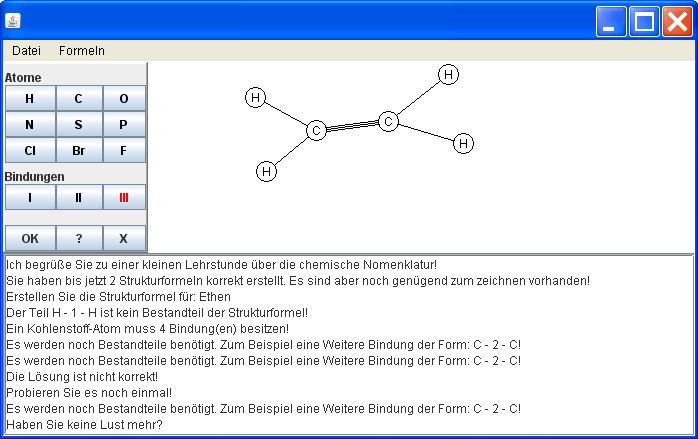
\includegraphics[width=0.7\linewidth,keepaspectratio]{bilder/chemnom.png}
	\caption{Das Programm \emph{ChemNom}}
	\label{fig:chemnom}
\end{figure}

Für diese Arbeit wird davon ausgegangen, dass die 
Modelle als Graphen vorliegen, da sich mit Graphen sehr 
viele Modelle darstellen lassen. 
Im Fall von \emph{ChemNom} würden die Moleküle als Graphen dargestellt, 
indem man die Atome als Knoten interpretiert und die Bindungen 
als Kanten.

Des Weiteren ist eine Musterlösung gegeben. Die Eingabe des 
Lerners soll dann mit der Musterlösung verglichen werden. 
Dabei stellt sich die Frage nach der Machbarkeit einer 
solchen Überprüfung.

\section{Korrektheit und Fehlergröße}
Die erste Frage, die sich stellt, ist: Wann ist eine 
eingegebene Lösung korrekt? Da eine Musterlösung vorliegt, 
wird eine Lösung als korrekt definiert, wenn sie mit der 
Musterlösung identisch ist. Falls es mehrere richtige Lösungen 
gibt, kann man mehrere Musterlösungen angeben.

Bei einem Lernprozess ist es jedoch vermutlich 
häufiger der Fall, dass die vorgeschlagene Lösung nicht 
korrekt ist. Um dem Lerner ein Feedback geben zu können, 
ist es somit nötig zusätzliche Aussagen über eine falsche 
Lösung zu treffen. Ein erster Ansatz ist dabei ein Maß, 
um zwischen verschiedenen Graden an fehlerhaften Lösungen 
zu unterscheiden. In dieser Arbeit sei dieses Maß der 
Aufwand, der nötig ist, um die Lösung des Lerners in die 
Musterlösung umzuwandeln. Dieser Aufwand wird als 
Graphabstand bezeichnet.

Um zu überprüfen, ob eine Lösung (des Lerners) korrekt ist 
oder um eine Aussage über die Fehler in einer Lösung zu 
treffen, ist es notwendig Knoten und Kanten der Lösung den 
entsprechenden Knoten und Kanten in der Musterlösung 
zuzuordnen. Dies ist nicht trivial. In \cite{Bravo:2006} 
wird das Problem damit umgangen, dass die Bezeichnung der 
Knoten in der Eingabe des Lerners mit Namenslisten abgeglichen 
wird, oder der Lerner selbst die Zuordnung vornimmt.

\section{Ziele und Anforderungen}
Ziel dieser Arbeit ist die Schaffung einer algorithmischen 
Grundlage, um in einer Modellierungsaufgabe den Lösungsvorschlag 
eines Lerners zu überprüfen und zu bewerten. Dabei soll die 
Zuordnung der Knoten zueinander automatisch erfolgen.

Für ein Verfahren zur Auswertung einer Lösung stellen sich 
dabei einige Anforderungen. Das Verfahren sollte möglichst 
unabhängig vom konkreten Modell arbeiten. Zusätzlich ist 
eine geringe Laufzeit wünschenswert. Im Idealfall bekommt 
der Lerner ohne spürbare Verzögerung eine Rückmeldung 
zu seiner Eingabe. Auch wenn die Berechnung länger dauert, 
sollte sie nicht mehr als ein paar Sekunden benötigen.

\section{Vorhaben}
Um die genannten Ziele zu erreichen, befasst sich diese Arbeit 
zuerst mit einigen Grundlagen im Bereich der Graphentheorie. 
Danach sollen verschiedene algorithmische Ansätze vorgestellt 
und untersucht werden. Fällt die Untersuchung positiv aus, dann 
wird zusätzlich ein Konzept vorgestellt, mit dem sich weitere 
Aussagen über die Eingabe eines Lerners treffen lassen.


\chapter{Theoretische Grundlagen und Begriffe}
Dieses Kapitel beinhaltet einen Überblick über Begriffe und Probleme, die in 
dieser Arbeit auftreten.

\section{Graphen und Teilgraphen}
%ToDo: (u,u) nicht erlauben
\begin{mydef}[Graph]Ein Graph $G$ ist ein 2-Tupel $G=(V,E)$. Dabei sind
\begin{itemize}
  \item $V$ eine endliche Menge von Knoten und
  \item $E \subseteq V \times V$ die Menge an Kanten.
\end{itemize}
Ist ein Graph \emph{ungerichtet}, dann gilt für jede Kante $e=(u,v) \in E:
(u,v)=(v,u)$. Im \emph{gerichteten} Fall gilt: $(u,v)\neq (v,u)$.
\end{mydef}

\begin{mydef}[Teilgraph]
Es sei $T=(V_t,E_t)$ ein Graph. $T$ ist Teilgraph des Graphen $G=(V,E)$ genau
dann, wenn die beiden nachfolgenden Bedingungen gelten:
\begin{itemize}
	\item $V_t \subseteq V$ 
	\item $e \in E_t \Rightarrow e \in E$
\end{itemize}
Gilt für alle $u,v \in V_t$ zusätzlich $(u,v) \in E \Rightarrow (u,v) \in E_t$, dann
ist $T$ ein \emph{induzierter} Teilgraph.\end{mydef}

Der Unterschied zwischen einem induzierten und nichtinduzierten 
Teilgraphen liegt darin, dass bei einem induzierten jede Kante 
zwischen zwei Knoten $u$ und $v$ enthalten sein muss ($(u,v) \in E_t 
\Leftrightarrow (u,v) \in E$). Bei einem nichtinduzierten Teilgraph 
ist dies optional ($(u,v) \in E_t \Rightarrow (u,v) \in E$). 
Abbildung \ref{pic:bsp_tg} stellt dies dar. Zwar ist $T$ ein (nichtinduzierter) Teilgraph 
von $G$, jedoch fehlt die Kante $(a,c)$, damit $T$ auch ein induzierter Teilgraph ist.


%\begin{figure}[htb]
%\centering
%\hspace*{\fill}
%\subfloat[]{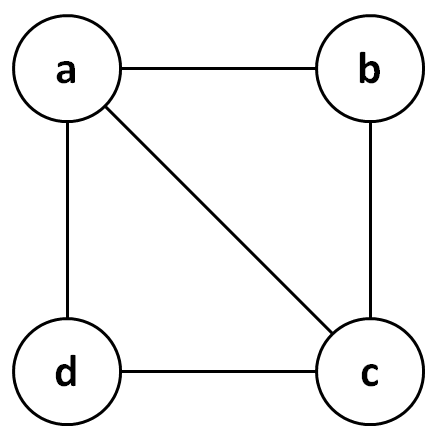
\includegraphics[width=0.3\linewidth,
%keepaspectratio]{bilder/bsp_tg_g}}
%\hspace*{\fill}
%\subfloat[]{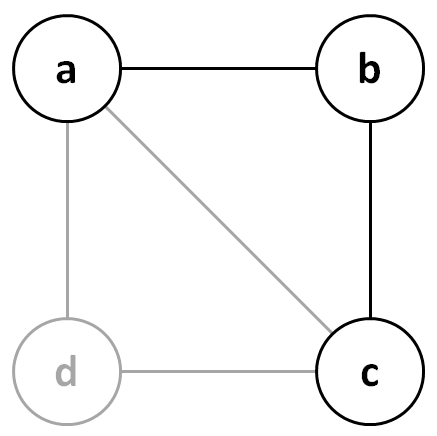
\includegraphics[width=0.3\linewidth,
%keepaspectratio]{bilder/bsp_tg_t}}
%\hspace*{\fill}
%\caption{Der Graph $G$ und dessen Teilgraph $T$}
%\label{pic:bsp_tg}
%\end{figure}

\begin{figure}[htb]
\centering
\hspace*{\fill}
\subfloat[]{\begin{tikzpicture}
  [normalN/.style={circle,draw,minimum size=0.8cm,thick},
   node distance=1.3cm]

  \node[normalN] (a) {a};
    
  \node[normalN] (b) [right=of a] {b}
    edge [thick] (a);
    
  \node[normalN] (c) [below=of b] {c}
    edge [thick] (b)
    edge [thick] (a);
    
  \node[normalN] (d) [left=of c] {d}
    edge [thick] (a)
    edge [thick] (c);

  
\end{tikzpicture}}
\hspace*{\fill}
\subfloat[]{\begin{tikzpicture}
  [normalN/.style={circle,draw,minimum size=0.8cm,thick},
   hiddenN/.style={circle,draw=black!33,black!33,minimum size=0.8cm,thick},
   node distance=1.3cm]

  \node[normalN] (a) {a};
    
  \node[normalN] (b) [right=of a] {b}
    edge [thick] (a);
    
  \node[normalN] (c) [below=of b] {c}
    edge [thick] (b)
    edge [thick,black!33] (a);
    
  \node[hiddenN] (d) [left=of c] {d}
    edge [thick,black!33] (a)
    edge [thick,black!33] (c);
  
\end{tikzpicture}}
\hspace*{\fill}
\caption{Der Graph $G$ und dessen Teilgraph $T$}
\label{pic:bsp_tg}
\end{figure}

\section{Graphisomorphie}
Graphisomorphie (GI) bezeichnet vereinfacht gesagt, ob zwei Graphen gleich
sind. Dies bedeutet bildlich gesprochen, dass man beide Graphen
übereinander legen kann.

\begin{mydef}[Graphisomorphie]
Zwei Graphen $G_1 = (V_1,E_1)$ und $G_2 = (V_2,E_2)$ heißen isomorph, wenn
eine bijektive Abbildung $\varphi: V_1 \rightarrow V_2$ existiert, so dass
für alle $u,v \in V_1$ gilt: $(u,v) \in E_1 \Leftrightarrow (\varphi(u),
\varphi(v)) \in E_2$.
\end{mydef}

Das zur GI gehörende Entscheidungsproblem fragt, ob für zwei gegebene 
Graphen eine oben genannte Abbildung existiert. Eine Besonderheit ist 
hierbei die Komplexität. Zwar liegt GI in NP\footnote{Ein Problem liegt 
in NP genau dann, wenn es mit einer nichtdeterministischen (Turing-)Maschine 
in polynomieller Zeit gelöst werden kann.} \cite{GIinNP}, jedoch konnte bis 
zum Zeitpunkt dieser Arbeit weder bewiesen noch widerlegt werden, ob es 
möglich ist, GI in Polynomialzeit zu lösen oder ob GI NP-vollständig\footnote{Ein 
Problem ist NP-vollständig genau dann, wenn es in NP liegt und sich jedes 
Problem in NP in Polynomialzeit darauf reduzieren lässt.} ist \cite{wikiD:GI,wikiE:GI}. 

Es ist also unbekannt, ob es einen Algorithmus gibt, der 
mit polynomiellem Aufwand überprüft, ob zwei Graphen isomorph sind.


\section{Teilgraphisomorphie}
Ähnlich zur einfachen GI gibt Teilgraphisomorphie (TGI) an, ob ein Graph 
$G_1$ isomorph zu einem Teilgraph von $G_2$ ist.

\begin{mydef}[Teilgraphisomorphie]
Ein Graph $G_1 = (V_1,E_1)$ ist isomorph zu einem Teilgraph von $G_2 =
(V_2,E_2)$ genau dann, wenn eine injektive Abbildung $\varphi: V_1
\rightarrow V_2$ existiert und für alle $u,v \in V_1$ gilt: $(u,v) \in E_1
\Rightarrow (\varphi(u),\varphi(v)) \in E_2$.
\end{mydef}

Analog zur GI wird auch beim TGI-Problem nach der Existenz einer in der 
Definition beschriebenen Abbildung gefragt. Das TGI-Problem ist 
NP-vollständig \cite{Cook:1971}.

\subsubsection{Anmerkung}
Im Rahmen dieser Arbeit wird in dem Fall, dass $G_1$ isomorph zu einem 
Teilgraph von $G_2$ ist, lediglich davon gesprochen, dass $G_1$ ein 
Teilgraph von $G_2$ ist. 


\section{Größter gemeinsamer Teilgraph}
Der größte gemeinsame Teilgraph (engl.: maximum common subgraph) 
zweier Graphen $G_1$ und $G_2$ beschreibt den größtmöglichen Graphen $H$, 
der Teilgraph von $G_1$ und $G_2$ ist.

\begin{mydef}[gemeinsamer Teilgraph (gTG)]\label{def:gTG} 
Ein Graph $H=(V_H,E_H)$ ist ein gemeinsamer Teilgraph von $G_1 = (V_1,E_1)$ und 
$G_2=(V_2,E_2)$ genau dann, wenn alle der vier nachflogenden Bedingungen 
erfüllt sind:
\begin{itemize}
  \item $V_H \subseteq V_1$
  \item $E_H \subseteq E_1$
	\item Es existiert eine injektive Abbildung $\varphi: V_H \rightarrow V_2$
	\item Für alle $u,v \in V_H$ gilt: $(u,v) \in E_H \Rightarrow (\varphi(u),
	      \varphi(v)) \in E_2$
\end{itemize}

Handelt es sich um einen gemeinsamen \emph{induzierten} Teilgraphen (giTG), 
dann gilt zusätzlich für alle $u,v \in V_H$: $(u,v) \in E_1 \Leftrightarrow 
(u,v) \in E_H \Leftrightarrow (\varphi(u),\varphi(v)) \in E_2$
\end{mydef}

\subsection{Der induzierte Fall}
Das Maß für die Größe des Teilgraphen ist abhängig davon, ob 
der giTG betrachtet wird oder lediglich der gTG. Im induzierten 
Fall ist die Anzahl der Knoten von $H$ das Größenmaß.

\begin{mydef}[größter gemeinsamer induzierter Teilgraph]
Sei $H=(V_H,E_H)$ ein giTG von $G_1$ und $G_2$. $H$ ist größter giTG von 
$G_1$ und $G_2$ genau dann, wenn kein giTG $H'=(V',E')$ von $G_1$ und $G_2$ 
existiert mit $|V'|>|V_H|$. Der größte giTG wird als MCS bezeichnet.
\end{mydef}

%\begin{figure}[htb]
%\centering
% %\hfill %
%\subfloat[]{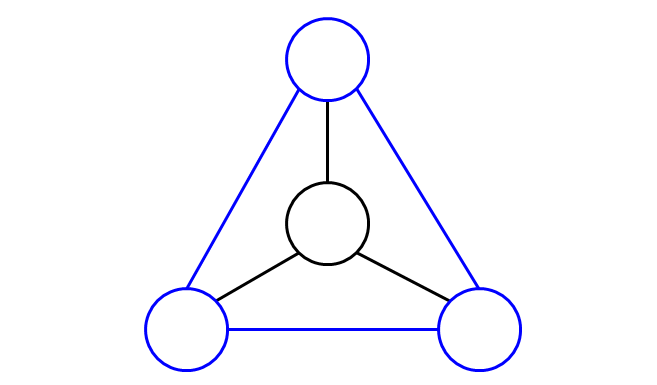
\includegraphics[width=0.4\linewidth,
%keepaspectratio]{bilder/bsp_giTG_g1}}
%\hspace{1.5cm} 
%\subfloat[]{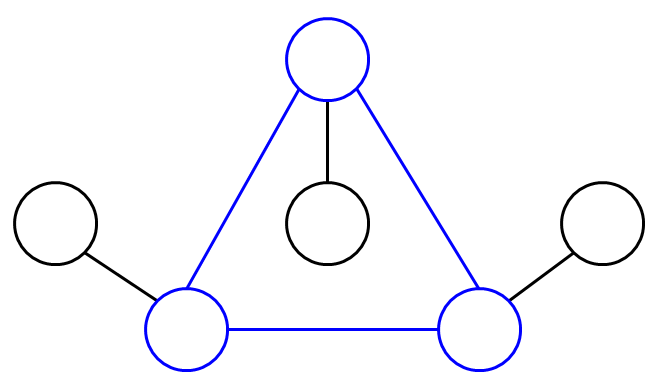
\includegraphics[width=0.4\linewidth,
%keepaspectratio]{bilder/bsp_giTG_g2}}
% %\hfill %
%\caption{Der MCS (blau) zweier Graphen}
%\label{pic:giTG}
%\end{figure}

\begin{figure}[htb]
\centering
\hspace*{\fill}
\subfloat[]{\begin{tikzpicture}
  [normalN/.style={circle,draw,minimum size=0.7cm,thick}]

  \node[normalN]      (center) at (0:0)     {};
  \node[normalN,blue] (top)    at (90:1.4)  {};
  \node[normalN,blue] (left)   at (210:1.4) {};
  \node[normalN,blue] (right)  at (-30:1.4) {};
  
  \draw [thick] (center) -- (top);
  \draw [thick] (center) -- (left);
  \draw [thick] (center) -- (right);
  
  \draw [thick,blue] (left) -- (right);
  \draw [thick,blue] (top) -- (right);
  \draw [thick,blue] (top) -- (left);
  
\end{tikzpicture}}
\hspace*{\fill}
\subfloat[]{\begin{tikzpicture}
  [normalN/.style={circle,draw,minimum size=0.7cm,thick},
   blueN/.style={normalN,blue}]

  \node[normalN] (center) at (0:0)    {};
  \node[blueN]   (top)    at (90:1.4) {};
  
  \path (210:1.4) node[blueN]   (left) {}
       +(120:1.4) node[normalN] (l)    {};
  

  \path (-30:1.4) node[blueN]   (right) {}
       +(60:1.4)  node[normalN] (r)     {};
  
  \draw [thick] (center) -- (top);
  %\draw [thick] (center) -- (left);
  %\draw [thick] (center) -- (right);
  
  \draw [thick,blue] (left) -- (right);
  \draw [thick,blue] (top) -- (right);
  \draw [thick,blue] (top) -- (left);
  
  \draw [thick] (left)  -- (l);
  \draw [thick] (right) -- (r);
\end{tikzpicture}}
\hspace*{\fill}
\caption{Der MCS (blau) zweier Graphen}
\label{pic:giTG}
\end{figure}

Das NP-vollständige \cite{Garey:1990} MCS-Problem stellt die folgende Frage: 
Existiert für zwei Graphen $G_1=(V_1,E_1)$ und $G_2=(V_2,E_2)$ sowie ein 
$k>0$ ein giTG $H=(V_H,E_H)$, für den gilt: $|V_H| \geq k$?


\subsection{Der allgemeine Fall}
Wird lediglich der gTG betrachtet, ist die Anzahl der Kanten das Maß 
für die Größe. Dies liegt daran, dass ein Graph $H$, der nur aus den 
Knoten des kleineren der Graphen $G_1$ und $G_2$ besteht, immer ein 
gTG von $G_1$ und $G_2$ ist. Zum größten gTG zweier Graphen gehören somit 
immer alle Knoten des kleineren Graphen.


\begin{myTheo}
Gegeben seien zwei Graphen $G_1 = (V_1,E_1)$ und $G_2=(V_2,E_2)$, wobei 
$|V_1| \leq |V_2|$. $H=(V_1,\emptyset)$ ist dann ein gTG von $G_1$ und $G_2$.
\end{myTheo}

\begin{myProof}
$H=(V_H,E_H)=(V_1,\emptyset)$ ist gTG von $G_1$ und $G_2$, wenn die folgenden 
Bedingungen (aus Definition \ref{def:gTG}) gelten:
\begin{enumerate}
  \item $V_H \subseteq V_1$
  \item $E_H \subseteq E_1$
	\item Es existiert eine injektive Abbildung $\varphi: V_H \rightarrow V_2$
	\item Für alle $u,v \in V_H$ gilt: $(u,v) \in E_H \Rightarrow (\varphi(u),
	      \varphi(v)) \in E_2$
\end{enumerate}

Die Bedingungen 1 ($V_1 \subseteq V_1$) und 2 ($\emptyset \subseteq E_1$) sind 
offensichtlich erfüllt.

Bedingung 3: Eine injektive Abbildung lässt sich dadurch erzeugen, dass jedem 
Knoten in $V_1$ ein Knoten in $V_2$ zugewiesen wird. Da $|V_1| \leq |V_2|$ ist 
es möglich jedem Knoten in $V_1$ einen anderen Knoten in $V_2$ zuzuordnen. 
Somit existiert immer eine injektive Abbildung.

Bedingung 4: Da $H$ keine Kanten besitzt ($E_H=\emptyset$), gilt für alle 
$u,v \in V_H$, dass $(u,v) \in E_H$ eine falsche Aussage ist. Somit ist die 
Implikation in Bedingung 4 immer wahr.

Alle Bedingungen sind erfüllt, somit ist $H$ ein gTG von $G_1$ und $G_2$. \qed
\end{myProof}

%\begin{figure}[htb]
%\centering
% %\hfill %
%\subfloat[]{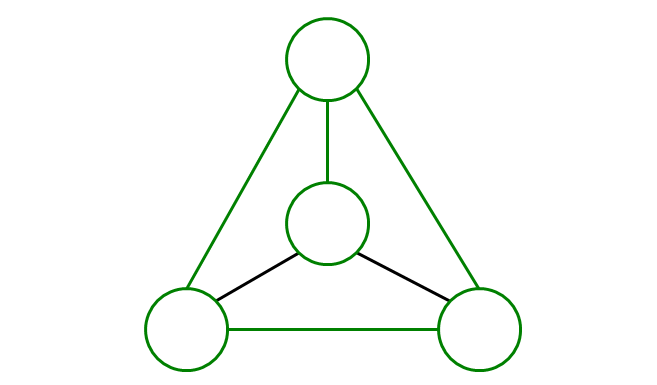
\includegraphics[width=0.4\linewidth,
%keepaspectratio]{bilder/bsp_gTG_g1}}
%\hspace{1.5cm} 
%\subfloat[]{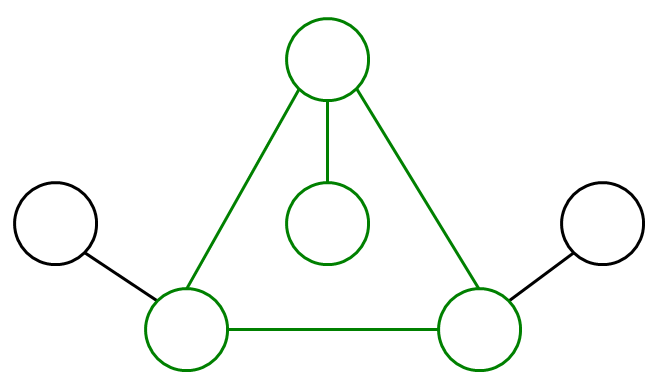
\includegraphics[width=0.4\linewidth,
%keepaspectratio]{bilder/bsp_gTG_g2}}
% %\hfill %
%\caption{Der größte gTG (grün) zweier Graphen}
%\label{pic:gTG}
%\end{figure}

\begin{figure}[htb]
\centering
\hspace*{\fill} 
\subfloat[]{\begin{tikzpicture}
  [normalN/.style={circle,draw,minimum size=0.7cm,thick}]

  \node[normalN,darkgreen] (center) at   (0:0)   {};
  \node[normalN,darkgreen] (top)    at  (90:1.4) {};
  \node[normalN,darkgreen] (left)   at (210:1.4) {};
  \node[normalN,darkgreen] (right)  at (-30:1.4) {};
  
  \draw [thick,darkgreen] (center) -- (top);
  \draw [thick] (center) -- (left);
  \draw [thick] (center) -- (right);
  
  \draw [thick,darkgreen] (left) -- (right);
  \draw [thick,darkgreen] (top) -- (right);
  \draw [thick,darkgreen] (top) -- (left);
  
\end{tikzpicture}}
\hspace*{\fill} 
\subfloat[]{\begin{tikzpicture}
  [normalN/.style={circle,draw,minimum size=0.7cm,thick},
   blueN/.style={normalN,darkgreen}]

  \node[blueN] (center) at (0:0)    {};
  \node[blueN]   (top)    at (90:1.4) {};
  
  \path (210:1.4) node[blueN]   (left) {}
       +(120:1.4) node[normalN] (l)    {};
  

  \path (-30:1.4) node[blueN]   (right) {}
       +(60:1.4)  node[normalN] (r)     {};
  
  \draw [thick,darkgreen] (center) -- (top);
  %\draw [thick] (center) -- (left);
  %\draw [thick] (center) -- (right);
  
  \draw [thick,darkgreen] (left) -- (right);
  \draw [thick,darkgreen] (top) -- (right);
  \draw [thick,darkgreen] (top) -- (left);
  
  \draw [thick] (left)  -- (l);
  \draw [thick] (right) -- (r);
\end{tikzpicture}}
\hspace*{\fill} 
\caption{Der größte gTG (grün) zweier Graphen}
\label{pic:gTG}
\end{figure}

\begin{mydef}[größter gemeinsamer Teilgraph]
Sei $H=(V_H,E_H)$ ein gTG von $G_1$ und $G_2$. $H$ ist größter gTG von 
$G_1$ und $G_2$ genau dann, wenn kein gTG $H'=(V',E')$ 
von $G_1$ und $G_2$ existiert mit $|E'|>|E_H|$
\end{mydef}


\section{Graphabstand}\label{sec:Graphabstand}
Als Graphabstand (engl.: graph edit distance) bezeichnet man die Kosten, 
die nötig sind, um einen Graphen so umzubauen, dass er isomorph zu einem 
anderen ist. 

Die Definitionen in diesem Abschnitt basieren auf den entsprechenden Definitionen 
in \cite{Bunke:1997}.

\begin{mydef}[error correcting graph matching (ECGM)]
Es seien $G_1=(V_1,E_1)$ und $G_2=(V_2,E_2)$ Graphen. Ein 
error correcting graph matching ist eine bijektive Abbildung 
$\varphi:\hat{V}_1 \rightarrow \hat{V}_2$ mit $\hat{V}_1 
\subseteq V_1$ und $\hat{V}_2 \subseteq V_2$.
\end{mydef}

Die Abbildung $\varphi$ stellt nun eine mögliche Bearbeitung von $G_1$ 
zu $G_2$ dar. Aus $G_1$, $G_2$ und $\varphi$ leiten sich ab: 
\begin{itemize}
	\item $V_d:=V_1 \backslash \hat{V}_1$ sind die zu löschenden Knoten,
	\item $V_a:=V_2 \backslash \hat{V}_2$ sind die hinzuzufügenden Knoten,
	\item $E_d:=E_1 \backslash \{(u,v) \ |\ u,v \in \hat{V}_1 \wedge (\varphi(u),
	       \varphi(v)) \in E_2\}$ sind die zu löschenden Kanten und
	\item $E_a:=E_2 \backslash \{(\varphi(u),\varphi(v))\ |\ u,v \in E_1 
	       \backslash E_d\}$ sind die hinzuzufügenden Kanten.
\end{itemize}

\begin{mydef}[Kosten eines ECGM]
Die Kosten eines ECGM $\varphi$ von $G_1$ nach $G_2$ seien definiert durch
\[
c(\varphi)=\sum_{v \in V_d}c_{nd}(v) + \sum_{v \in V_a}c_{na}(v) + 
  \sum_{e \in E_a}c_{ed}(e) + \sum_{e \in E_d}c_{ea}(e).
\]
Dabei seien: 
\begin{itemize}
	\item $c_{nd}(v) \geq 0$ die Kosten für das Löschen eines Knotens,
	\item $c_{na}(v) \geq 0$ die Kosten für das Hinzufügen eines Knotens,
	\item $c_{ed}(e) \geq 0$ die Kosten für das Löschen einer Kante und
	\item $c_{ea}(e) \geq 0$ die Kosten für das Hinzufügen einer Kante.
\end{itemize}
\end{mydef}

Es ist möglich, die Kostenfunktion zu erweitern. Besitzt ein Graph 
beispielsweise eine Beschriftung oder Gewichtung (dies können z.B. 
Entfernungen in einem Straßennetz sein), so ist das Editieren eines 
Knotens oder einer Kante möglich. Dabei entfernt man die Kante nicht, 
sondern ändert lediglich die Beschriftung oder das Gewicht. 

\begin{mydef}[Graphabstand]
Der Graphabstand $d(G_1,G_2)$ für zwei Graphen $G_1$ und $G_2$ sei 
definiert durch die minimalen Kosten über allen möglichen ECGMs von $G_1$ 
nach $G_2$.
\[
d(G_1,G_2):=\min\{c(\varphi)\ |\ \varphi \text{ ist ein ECGM von } G_1 
\text{ nach } G_2\}
\]
\end{mydef}

\subsubsection{Graphabstand als Entscheidungsproblem}
Gegeben seien zwei Graphen $G_1$ und $G_2$ sowie ein $k$. Existiert ein 
ECGM $\varphi$ von $G_1$ nach $G_2$ mit $c(\varphi) \leq k$?

Garaphabstand ist NP-vollständig. \cite{GEDisNPcomp}


\section{Zusammenhang von MCS und Graphabstand}\label{sec:MCS_Graphabstand}
In \cite{Bunke:1997} wird gezeigt, dass bei geeigneter Wahl der Kosten 
der Graphabstand zweier Graphen $G_1=(V_1,E_1)$ und $G_2=(V_2,E_2)$ 
durch die Größe des MCS $G=(V,E)$ berechnet werden kann. Es gilt dann:

\begin{equation}
d(G_1,G_2)=|V_1| + |V_2| - 2 |V|\label{form:mcs}
\end{equation}

Der Graphabstand kann somit ermittelt werden, indem man den MCS zweier 
Graphen bildet. Knoten und Kanten, die nicht zum MCS gehören werden entfernt 
oder hinzugefügt.

Die Kostenfunktionen $c_{nd}(v)$, $c_{na}(v)$, $c_{ed}(e)$, und $c_{ea}(e)$, 
die in \cite{Bunke:1997} angegeben wurden, damit (\ref{form:mcs}) gilt, sind 
(angepasst an die in dieser Arbeit verwendeten Definitionen eines 
Graphen und Kosten eines ECGMs) wie folgt definiert:

\begin{itemize}
	\item $c_{na}(v)=1$
	\item $c_{nd}(v)=1$
	\item $c_{ed}(e)=\left\{\begin{array}{ll}\infty & e \in \hat{V}_1 \times 
	                  \hat{V}_1\\0 & \text{sonst}\end{array}\right. $
	\item $c_{ea}(e)=\left\{\begin{array}{ll}\infty & e \in \hat{V}_2 \times 
	                  \hat{V}_2\\0 & \text{sonst}\end{array}\right. $
\end{itemize}

\subsection{Probleme bei der Nutzung}
Beim Ermitteln des Graphabstands mittels des MCS und der oben beschriebenen 
Kostenfunktion ergeben sich Probleme.

Die Kosten für das Hinzufügen und Entfernen von Kanten sind entweder $0$ oder 
unendlich. Solange der Graphabstand endlich ist, ist er somit unabhängig von 
der Anzahl der Kanten, die hinzugefügt oder entfernt werden müssen.

Ein weiteres Problem ist, dass alle Knoten, die nicht zum MCS gehören, entfernt 
oder hinzugefügt werden. Es kann jedoch Fälle geben, in denen das nicht erwünscht 
ist. Abbildung \ref{pic:bspMCS_GED} stellt einen solchen Fall dar. Der MCS ist 
dabei \emph{grün} markiert.

%\begin{figure}[htb]
%\centering
%\hspace*{\fill} 
%\subfloat[Eingabe des Lerners]{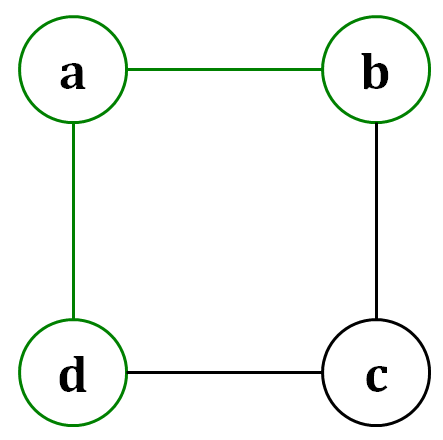
\includegraphics[width=0.25\linewidth,
%keepaspectratio]{bilder/bsp_msc_ged_1}}
%\hspace*{\fill} 
%\subfloat[Musterlösung]{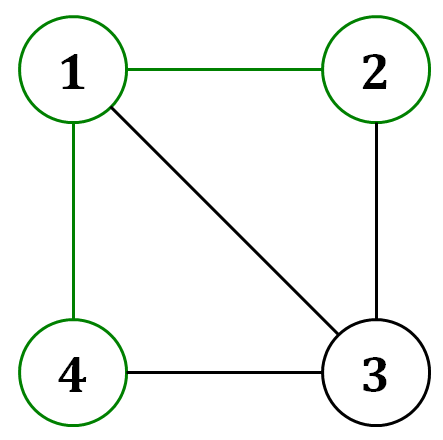
\includegraphics[width=0.25\linewidth,
%keepaspectratio]{bilder/bsp_msc_ged_2}}
%\hspace*{\fill} 
%\caption{Beispiel für einen ungüstigen MCS (grün) zweier Graphen}
%\label{pic:bspMCS_GED}
%\end{figure}

\begin{figure}[htb]
\centering
\hspace*{\fill} 
\subfloat[Eingabe des Lerners]{\begin{tikzpicture}
  [normalN/.style={circle,draw,minimum size=0.8cm,thick},
   greenN/.style={circle,draw=darkgreen,minimum size=0.8cm,thick},
   node distance=1.3cm]

  \node[greenN] (a) {a};
    
  \node[greenN] (b) [right=of a] {b}
    edge [thick,darkgreen] (a);
    
  \node[normalN] (c) [below=of b] {c}
    edge [thick] (b);
    
  \node[greenN] (d) [left=of c] {d}
    edge [thick,darkgreen] (a)
    edge [thick] (c);
  
\end{tikzpicture}}
\hspace*{\fill} 
\subfloat[Musterlösung]{\begin{tikzpicture}
  [normalN/.style={circle,draw,minimum size=0.8cm,thick},
   greenN/.style={circle,draw=darkgreen,minimum size=0.8cm,thick},
   node distance=1.3cm]

  \node[greenN] (a) {1};
    
  \node[greenN] (b) [right=of a] {2}
    edge [thick,darkgreen] (a);
    
  \node[normalN] (c) [below=of b] {3}
    edge [thick] (b)
    edge [thick] (a);
    
  \node[greenN] (d) [left=of c] {4}
    edge [thick,darkgreen] (a)
    edge [thick] (c);
  
\end{tikzpicture}}
\hspace*{\fill} 
\caption{Beispiel für einen ungünstigen MCS (grün) zweier Graphen}
\label{pic:bspMCS_GED}
\end{figure}

Der Fehler des Lerners in Abbildung \ref{pic:bspMCS_GED} ist lediglich eine 
fehlende Kante. Ermittelt man nun den Graphabstand mittels des MCS, so wird 
der Knoten~$c$ entfernt und Knoten~$3$ hinzugefügt. Somit wird Knoten~$c$ als 
fehlerhaft und Knoten~$3$ als fehlend betrachtet.

\subsection{Kantengraphen}
Kantengraphen sind ein für diese Arbeit erdachtes Konzept. Die Idee 
daran ist, in einem gegebenen Graphen die Kanten durch zusätzliche 
Knoten darzustellen. Der Kantengraph $K$ eines Graphen $G=(V,E)$ ergibt 
sich, indem man jede Kante $e=(u,v) \in E$ zur Knotenmenge hinzugefügt 
und der so entstandene Knoten mit den "`alten"' Knoten $u$ und $v$ 
verbunden wird. Abbildung \ref{pic:bspKantengraph} stellt dies dar.

\begin{mydef}[Kantengraph]\label{def:Kantengraph}
Für einen gegebenen Graphen $G=(V,E)$ sei dessen Kantengraph $K$ wie folgt 
definiert: 
\[
K=(V \cup E, \{(u,e),(e,v)\ |\ e=(u,v) \in E\})
\]
Die Funktion $k$ gibt den Kantengraph des übergeben Graphen zurück. 
\[ k(G)=K \]
\end{mydef}

%\begin{figure}[htb]
%\centering
% %\hspace*{\fill} 
%\subfloat[Original]{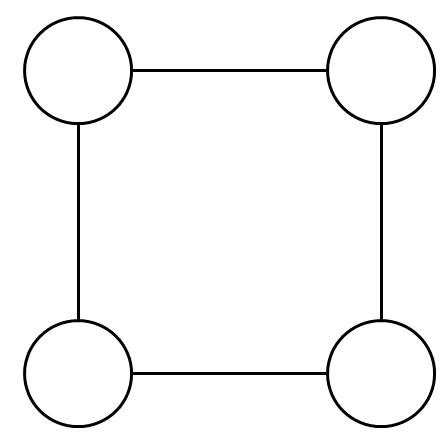
\includegraphics[width=0.25\linewidth,
%keepaspectratio]{bilder/bspKantengraph_1}}
%\hspace*{\fill} 
%\subfloat[Kanten in Knoten umwandeln]{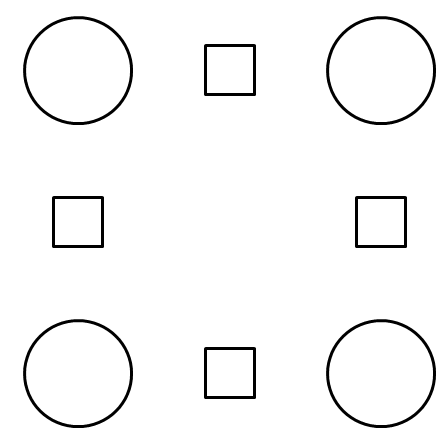
\includegraphics[width=0.25\linewidth,
%keepaspectratio]{bilder/bspKantengraph_2}}
%\hspace*{\fill} 
%\subfloat[neue Kanten]{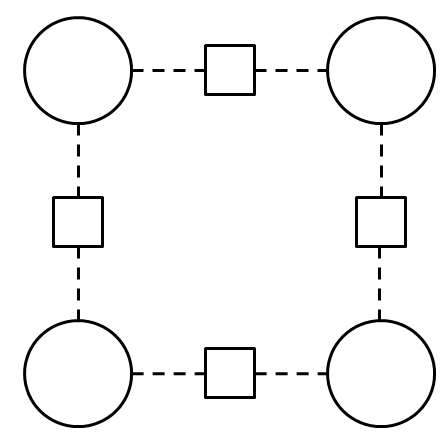
\includegraphics[width=0.25\linewidth,
%keepaspectratio]{bilder/bspKantengraph_3}}
% %\hspace*{\fill} 
%\caption{Erstellen eines Kantengraphen}
%\label{pic:bspKantengraph}
%\end{figure}

\begin{figure}[htb]
\centering
%\hspace*{\fill} 
\subfloat[Original]{\begin{tikzpicture}
  [normalN/.style={circle,draw,minimum size=0.8cm,thick},
   node distance=1.3cm]

  \node[normalN] (a) {};
    
  \node[normalN] (b) [right=of a] {}
    edge [thick] (a);
    
  \node[normalN] (c) [below=of b] {}
    edge [thick] (b);
    
  \node[normalN] (d) [left=of c] {}
    edge [thick] (a)
    edge [thick] (c);
  
\end{tikzpicture}}
\hspace*{\fill} 
\subfloat[Kanten in Knoten umwandeln]{\begin{tikzpicture}
  [normalN/.style={circle,draw,minimum size=0.8cm,thick},
   edgeN/.style={draw,minimum size=0.4cm,thick},
   node distance=0.45cm]

  \node[normalN] (a)                {};
  \node[edgeN]   (ab) [right=of a]  {};
  \node[normalN] (b)  [right=of ab] {};

  \node[edgeN]   (ad) [below=of a]  {};
  \node[edgeN]   (bc) [below=of b]  {};

  \node[normalN] (d)  [below=of ad] {};
  \node[edgeN]   (cd) [right=of d]  {};
  \node[normalN] (c)  [right=of cd] {};

\end{tikzpicture}}
\hspace*{\fill} 
\subfloat[neue Kanten]{\begin{tikzpicture}
  [normalN/.style={circle,draw,minimum size=0.8cm,thick},
   edgeN/.style={draw,minimum size=0.4cm,thick},
   node distance=0.45cm]

  \node[normalN] (a)                {};
  \node[edgeN]   (ab) [right=of a]  {};
  \node[normalN] (b)  [right=of ab] {};

  \node[edgeN]   (ad) [below=of a]  {};
  \node[edgeN]   (bc) [below=of b]  {};

  \node[normalN] (d)  [below=of ad] {};
  \node[edgeN]   (cd) [right=of d]  {};
  \node[normalN] (c)  [right=of cd] {};

  \draw[thick,dashed] (a) -- (ab);
  \draw[thick,dashed] (a) -- (ad);
  \draw[thick,dashed] (b) -- (ab);
  \draw[thick,dashed] (b) -- (bc);
  \draw[thick,dashed] (c) -- (bc);
  \draw[thick,dashed] (c) -- (cd);
  \draw[thick,dashed] (d) -- (ad);
  \draw[thick,dashed] (d) -- (cd);
\end{tikzpicture}
}
%\hspace*{\fill} 
\caption{Erstellen eines Kantengraphen}
\label{pic:bspKantengraph}
\end{figure}

Mit Hilfe eines Kantengraphen lassen sich nun die oben genannten 
Probleme umgehen. Dazu sucht man nicht den MCS der ursprünglichen 
Graphen, sondern den MCS der Kantengraphen. Dabei gilt es aber zu 
beachten, dass man Knoten, die eine Kante darstellen und normale 
Knoten nicht einander zuordnet.

Ein Problem der ursprünglichen Graphen war, dass Kanten nicht 
bewertet wurden. Da jede Kante nun als Knoten betrachtet wird, 
wird somit auch jede Kante in die Kosten für den Graphabstand 
eingerechnet. 

Ein weiteres Problem war, dass der MCS ein induzierter Teilgraph ist, 
wodurch Knoten ungewollt als fehlerhaft betrachtet werden können. Dieses 
Problem ist nun nicht mehr relevant, da jeder Teilgraph von $G$ ein 
induzierter Teilgraph von dessen Kantengraph $K$ ist. In dem 
Beispiel aus Abbildung~\ref{pic:bspMCS_GED} würden somit auch 
Knoten $c$ und $3$ zum MCS gehören.

\begin{myTheo}
Wenn $T$ ein Teilgraph des Graphen $G$ ist, dann ist $k(T)$ ein 
induzierter Teilgraph von $k(G)$.
\end{myTheo}

\begin{myProof}
Gegeben seien die Graphen $G=(V_g,E_g)$ sowie $T=(V_t,E_t)$. $T$ ist 
Teilgraph von $G$. $k(G)=(V_{kg},E_{kg})$ und $k(T)=(V_{kt},E_{kt})$ 
sind Kantengraphen von $G$ und $T$. 

Da $T$ Teilgraph von $G$ ist, gilt:
\begin{align*}
V_t &\subseteq V_g \\%\label{proForm:Knoten_T_G}\\
e \in E_t &\Rightarrow e \in E_g %\label{proForm:Kanten_T_G}
\end{align*}

Daraus folgt, dass $E_t \subseteq E_g$. Somit 
gilt auch:
\[ V_t \cup E_t \subseteq V_g \cup E_g \]

Da dies nach Definition \ref{def:Kantengraph} jeweils die Knotenmengen 
der Kantengraphen $k(G)$ und $k(T)$ sind, folgt daraus, dass die Knoten 
von $k(T)$ eine Teilmenge der Knoten von $k(G)$ darstellen.
\begin{equation}
V_{kt} \subseteq V_{kg} \label{proForm:Knotenbed}
\end{equation}

Für jede Kante $e=(u,v)$ gilt:
\begin{align}
e=(u,v) \in E_t &\Leftrightarrow (u,e) \in E_{kt} \text{ und } 
  (e,v) \in E_{kt} \label{proForm:Kanten_T} \\
e=(u,v) \in E_g &\Leftrightarrow (u,e) \in E_{kg} \text{ und } 
  (e,v) \in E_{kg} \label{proForm:Kanten_G}
\end{align}

Da aus der linken Seite von (\ref{proForm:Kanten_T}) die linke Seite 
von (\ref{proForm:Kanten_G}) folgt ($T$ ist Teilgraph von $G$) und die 
linke Seite jeweils äquivalent zur rechten ist, gilt somit, dass jede 
Kante $\varepsilon$ in $E_{kt}$ auch in $E_{kg}$ vorhanden ist.
\begin{equation}
\varepsilon \in E_{kt} \Rightarrow \varepsilon \in E_{kg} \label{proForm:Kantenbed}
\end{equation}

Aus (\ref{proForm:Knotenbed}) und (\ref{proForm:Kantenbed}) folgt, dass 
$k(T)$ ein Teilgraph von $k(G)$ ist. Es bleibt zu zeigen, dass es 
sich dabei um einen induzierten Teilgraphen handelt.

Es sei $\varepsilon$ eine Kante in $E_{kg}$, dessen Knoten in $V_{kt}$ sind. 
Nun gibt es zwei Fälle: $\varepsilon=(u,e)$ und $\varepsilon=(e,v)$, wobei 
$u,v \in V_t$ und $e=(u,v) \in E_t$.

Da $e=(u,v)$ eine Kante in T ist, sind auch $(u,e)$ und 
$(e,v)$ Kanten in $k(T)$. 
Somit ergibt sich, dass für alle $u^{*},v^{*} \in V_{kt}$ gilt: 
$(u^{*},v^{*}) \in E_{kg} \Rightarrow (u^{*},v^{*}) \in E_{kt}$. 
Somit ist $k(T)$ ein induzierter Teilgraph von $k(G)$. \qed
\end{myProof}

\subsection{Nachteile des Kantengraphen}
Kantengraphen besitzen zwei Nachteile. Dies sind ihre erhöhte Größe 
und ein Phänomen, das bei der Ermittlung eines MCS auftreten kann.

\subsubsection{Phänomen der freien Kanten}
Ermittelt man den MCS zweier Kantengraphen, gibt es ein Phänomen, 
das auftreten kann: \emph{freie Kanten}.

Die Kanten in einem Graphen $G$ werden in dessen Kantengraph $k(G)$ 
als Knoten dargestellt. Bei der Suche nach einem MCS sind diese dann 
gleichwertig mit "`normalen"' Knoten. Es nun möglich, dass eine 
Kante $e$ aus $G$, die ein Knoten in $k(G)$ darstellt, zum MCS gehört, 
die dazugehörigen Knoten jedoch nicht. Eine solche Kannte $e$ sei 
eine \emph{freie Kante}. Das Beispiel in Abbildung \ref{pic:bspFreieKanten} 
stellt dies dar. Die freien Kanten sind \emph{grün} markiert.

%\begin{figure}[htb]
%\centering
%\hspace*{\fill} 
%\subfloat[Graph $G_1$]{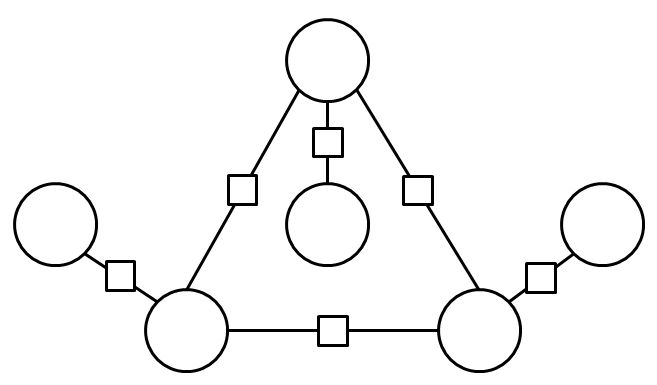
\includegraphics[width=0.4\linewidth,
%keepaspectratio]{bilder/bsp_mcs_kg_1}}
%\hspace*{\fill} 
%\subfloat[Graph $G_2$]{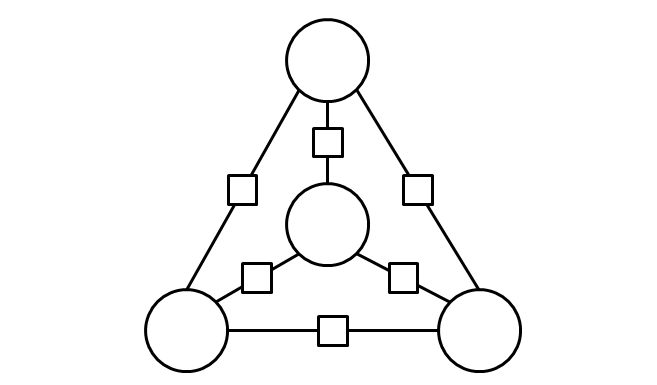
\includegraphics[width=0.4\linewidth,
%keepaspectratio]{bilder/bsp_mcs_kg_2}}
%\hspace*{\fill} \\ \hspace*{\fill} 
%\subfloat[MCS von $G_1$ und $G_2$]{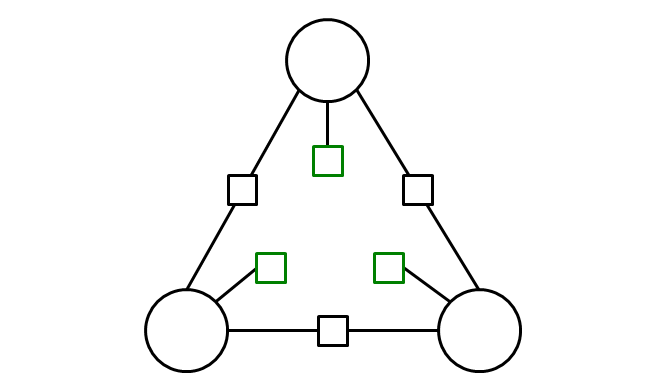
\includegraphics[width=0.4\linewidth,
%keepaspectratio]{bilder/bsp_mcs_kg_3}} \hspace*{\fill} 
%\caption{Das Phänomen der freien Kanten}
%\label{pic:bspFreieKanten}
%\end{figure}

\begin{figure}[htb]
\centering
\hspace*{\fill} 
\subfloat[Graph $G_1$]{\begin{tikzpicture}
  [normalN/.style={circle,draw,minimum size=0.7cm,fill=white},
   edgeN/.style={draw,minimum size=0.3cm,fill=white},
   thick]

  \coordinate (c) at (0:0);
  \coordinate (t) at (90:1.6);
  \coordinate (l) at (210:1.6);
  \coordinate (r) at (-30:1.6);
  
  \coordinate (cor_tr) at (30:0.8);
  \coordinate (cor_tl) at (150:0.8);
  \coordinate (cor_lr) at (-90:0.8);
  
  \coordinate (cor_ct) at  (90:0.8);
  \coordinate (cor_cl) at (210:0.8);
  \coordinate (cor_cr) at (-30:0.8);

  \draw [] (c) -- (cor_ct); \draw [] (t) -- (cor_ct);
  \draw [] (c) -- (cor_cl); \draw [] (l) -- (cor_cl);
  \draw [] (c) -- (cor_cr); \draw [] (r) -- (cor_cr);
  
  \draw [] (l) -- (cor_lr); \draw [] (r) -- (cor_lr);
  \draw [] (t) -- (cor_tl); \draw [] (l) -- (cor_tl);
  \draw [] (t) -- (cor_tr); \draw [] (r) -- (cor_tr);
  
  \path (210:1.6)+(120:1.6) node[normalN,draw=black!0] (ll) {};
  \path (-30:1.6)+ (60:1.6) node[normalN,draw=black!0] (rr) {};

  \node[normalN]  at   (0:0)   {};
  \node[normalN]  at  (90:1.6) {};
  \node[normalN]  at (210:1.6) {};
  \node[normalN]  at (-30:1.6) {};
  
  \node[edgeN] (etr) at  (cor_tr) {};
  \node[edgeN] (etl) at (150:0.8) {};
  \node[edgeN] (elr) at (-90:0.8) {};

  \node[edgeN] (ect) at  (90:0.8) {};
  \node[edgeN] (ecl) at (210:0.8) {};
  \node[edgeN] (ecr) at (-30:0.8) {};

  %\path (210:1.6)+(120:0.8) node[edgeN] (ell) {};
  %\path (-30:1.6)+ (60:0.8) node[edgeN] (err) {};

  
  %\draw [] (l) -- (ell); \draw [] (ll) -- (ell);
  %\draw [] (r) -- (err); \draw [] (rr) -- (err);
\end{tikzpicture}}
\hspace*{\fill} 
\subfloat[Graph $G_2$]{\begin{tikzpicture}
  [normalN/.style={circle,draw,minimum size=0.7cm,fill=white},
   edgeN/.style={draw,minimum size=0.3cm,fill=white},
   thick]

  \coordinate (c) at (0:0);
  \coordinate (t) at (90:1.6);
  \coordinate (l) at (210:1.6);
  \coordinate (r) at (-30:1.6);
  
  \coordinate (cor_tr) at (30:0.8);
  \coordinate (cor_tl) at (150:0.8);
  \coordinate (cor_lr) at (-90:0.8);
  
  \coordinate (cor_ct) at  (90:0.8);
  \coordinate (cor_cl) at (210:0.8);
  \coordinate (cor_cr) at (-30:0.8);

  \coordinate (cor_ll) at ($(210:1.6)+(120:0.8)$);
  \coordinate (cor_rr) at ($(-30:1.6)+ (60:0.8)$);

  \path (210:1.6)+(120:1.6) node[normalN] (ll) {};
  \path (-30:1.6)+ (60:1.6) node[normalN] (rr) {};
  
  \draw [] (c) -- (cor_ct); \draw [] (t) -- (cor_ct);
  
  \draw [] (l) -- (cor_lr); \draw [] (r) -- (cor_lr);
  \draw [] (t) -- (cor_tl); \draw [] (l) -- (cor_tl);
  \draw [] (t) -- (cor_tr); \draw [] (r) -- (cor_tr);
  
  \draw [] (l) -- (cor_ll); \draw [] (ll) -- (cor_ll);
  \draw [] (r) -- (cor_rr); \draw [] (rr) -- (cor_rr);

  \node[normalN]  at   (0:0)   {};
  \node[normalN]  at  (90:1.6) {};
  \node[normalN]  at (210:1.6) {};
  \node[normalN]  at (-30:1.6) {};
  
  \node[edgeN] (etr) at  (30:0.8) {};
  \node[edgeN] (etl) at (150:0.8) {};
  \node[edgeN] (elr) at (-90:0.8) {};

  \node[edgeN] (ect) at  (90:0.8) {};
  %\node[edgeN] (ecl) at (210:0.8) {};
  %\node[edgeN] (ecr) at (-30:0.8) {};

  \path (210:1.6)+(120:0.8) node[edgeN] (ell) {};
  \path (-30:1.6)+ (60:0.8) node[edgeN] (err) {};

\end{tikzpicture}
}
\hspace*{\fill} \\ \hspace*{\fill} 
\subfloat[MCS von $G_1$ und $G_2$]{\begin{tikzpicture}
  [normalN/.style={circle,draw,minimum size=0.7cm,fill=white},
   edgeN/.style={draw,minimum size=0.3cm,fill=white},
   thick]

  \coordinate (c) at (0:0);
  \coordinate (t) at (90:1.6);
  \coordinate (l) at (210:1.6);
  \coordinate (r) at (-30:1.6);
  
  \coordinate (cor_tr) at (30:0.8);
  \coordinate (cor_tl) at (150:0.8);
  \coordinate (cor_lr) at (-90:0.8);
  
  \coordinate (cor_ct) at  (90:0.8);
  \coordinate (cor_cl) at (210:0.8);
  \coordinate (cor_cr) at (-30:0.8);

  %\path (210:1.6)+(120:1.6) node[normalN] (ll) {};
  %\path (-30:1.6)+ (60:1.6) node[normalN] (rr) {};

  \draw [] (t) -- (cor_ct);
  \draw [] (l) -- (cor_cl);
  \draw [] (r) -- (cor_cr);
  
  \draw [] (l) -- (cor_lr); \draw [] (r) -- (cor_lr);
  \draw [] (t) -- (cor_tl); \draw [] (l) -- (cor_tl);
  \draw [] (t) -- (cor_tr); \draw [] (r) -- (cor_tr);
  
  %\node[normalN] (c) at   (0:0)   {};
  \node[normalN]  at  (90:1.6) {};
  \node[normalN]  at (210:1.6) {};
  \node[normalN]  at (-30:1.6) {};
  
  \node[edgeN] (etr) at  (30:0.8) {};
  \node[edgeN] (etl) at (150:0.8) {};
  \node[edgeN] (elr) at (-90:0.8) {};

  \node[edgeN,draw=darkgreen] (ect) at  (90:0.8) {};
  \node[edgeN,draw=darkgreen] (ecl) at (210:0.8) {};
  \node[edgeN,draw=darkgreen] (ecr) at (-30:0.8) {};

  %\path (210:1.6)+(120:0.8) node[edgeN] (ell) {};
  %\path (-30:1.6)+ (60:0.8) node[edgeN] (err) {};

  
  %\draw [] (l) -- (ell); \draw [] (ll) -- (ell);
  %\draw [] (r) -- (err); \draw [] (rr) -- (err);
\end{tikzpicture}} \hspace*{\fill} 
\caption{Das Phänomen der freien Kanten}
\label{pic:bspFreieKanten}
\end{figure}

\subsubsection{Größe des Kantengraphen}
Ein weiterer Nachteil ist, dass die Knotenzahl deutlich steigt. Da sowohl 
das Ermitteln des MCS als auch des Graphabstands NP-vollständig ist, 
gibt es vermutlich keinen Algorithmus in polynomieller Laufzeit sondern 
nur mit exponentieller. Ein Anstieg der Knoten und Kanten kann sich 
somit deutlich auf die Laufzeit auswirken.

%\section{Cliquen und unabhängige Mengen}
%Cliquen und unabhängige Mengen (engl.: independent set) sind besondere
%Mengen in Graphen. Eine Clique ist ein Graph, dessen Knoten alle miteinander
%verbunden sind. Im Gegensatz dazu ist ein independent set eine Menge von
%Knoten, zwischen denen keine Kante existiert.
%
%\begin{mydef}[Clique]
%Es seien $G=(V,E)$ ein ungerichteter Graph und $C=(V_c,E_c)$ 
%ein Teilgraph von $G$. $C$ ist eine Clique in $G$ genau dann, wenn 
%für alle $u$ und $v$ ($,v \in V_c$; $u\neq v$) gilt: $(u,v) \in E_c$.
%\end{mydef}
%
%\begin{mydef}[independent set]
%Sei $G=(V,E)$ ein ungerichteter Graph. $V_i \subseteq V$ ist
%ein independent set in $G \Leftrightarrow \forall e \in V_i \times 
%V_i: e \notin E$.
%\end{mydef}
%
%\begin{mydef}[Komplementärgraph]
%Sei $G=(V,E)$ ein Graph. $\overline{G}=(V,(V \times V) \backslash E)$ wird 
%als Komplementärgraph von $G$ bezeichnet.
%%ToDo: (u,u) nicht erlauben
%\end{mydef}
%
%Das Finden einer maximalen Clique oder eines maximalen independent sets
%(MIS) sind äquivalente Probleme. Dies liegt daran, dass eine Clique in $G$
%auch automatisch ein independent set im Komplementärgraphen $\overline{G}$
%darstellt. Aus der NP-Vollständigkeit des Findens der maximalen Clique
%\cite{Karp72} folgt somit, dass auch die Ermittlung des maximalen
%independent sets NP-vollständig ist.

\section{MCS und Assoziationsgraphen}\label{sec:MIS_MCS}
Das Finden eines MCS zweier Graphen lässt sich auf die Suche nach 
einer unabhängigen Menge (engl.: independent set) reduzieren \cite{MaxCSwitMaxIS}. 
Dazu erstellt man aus den gegebenen Graphen einen 
Assoziationsgraphen (AG). In diesem sucht man dann nach einem maximalen 
independent set.

\subsection{Unabhängige Menge}
Eine Unabhängige Menge in einem Graphen ist eine Teilmenge der Knoten des 
Graphen, wobei zwischen den Knoten keine Kante vorhanden ist.

\begin{mydef}[independent set]
Sei $G=(V,E)$ ein ungerichteter Graph. $V_i \subseteq V$ ist 
ein independent set in $G$ genau dann, wenn für alle $e \in V_i \times 
V_i$ gilt: $e \notin E$.
\end{mydef}

Das Ermitteln des maximum independent set (MIS) ist NP-vollständig \cite{Garey:1990}.

\subsection{Assoziationsgraph}
Ein gemeinsamer induzierter Teilgraph ist eine Abbildung der Knoten 
von einem Graphen $G_1$ auf die Knoten eines Graphen $G_2$ (siehe Definition \ref{def:gTG}). 
Die Idee des AGs ist es, jede mögliche Zuordnung, die zu einer 
solchen Abbildung gehören kann, in einem Graphen darzustellen.

%\begin{figure}[htb]
%\centering
%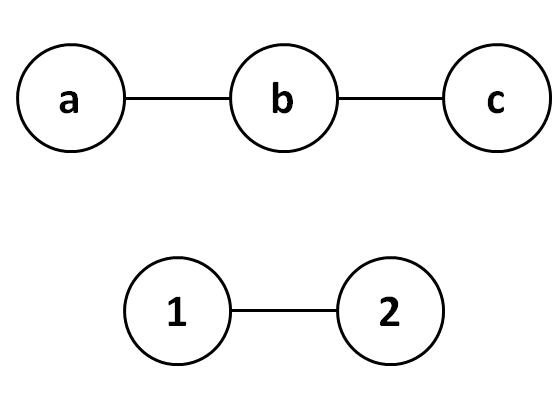
\includegraphics[width=0.4\linewidth,keepaspectratio]{bilder/bsg_ag_graphs.png}
%\caption{Die Graphen $G_1$ (oben) und $G_2$ (unten)}
%\label{pic:bsg_ag_graphs}
%\end{figure}

\begin{figure}[htb]
\centering
\vspace{0.5cm}
\begin{tikzpicture}
  [normalN/.style={circle,draw,minimum size=0.8cm,thick},
   node distance=0.8cm]

  \path (0,0)     node[normalN] (a) {a}
       +(0.8,-1.6) node[normalN] (1) {1};
       
  \node[normalN] (b) [right=of a] {b};
  \node[normalN] (c) [right=of b] {c};
  \node[normalN] (2) [right=of 1] {2};
    
  \draw [thick] (a) -- (b);
  \draw [thick] (b) -- (c);
  \draw [thick] (1) -- (2);
    
\end{tikzpicture}
\caption{Die Graphen $G_1$ (oben) und $G_2$ (unten)}
\label{pic:bsg_ag_graphs}
\end{figure}

Die Knoten des AGs stellen die möglichen Zuordnungen von einem Knoten auf 
einen anderen dar. Jeder Knoten ist somit ein Paar aus einem Knoten aus $G_1$ 
und einem Knoten aus $G_2$. Abbildung \ref{pic:bsg_ag_nodes} stellt die Kantenmenge des AGs 
dar, der sich aus den Graphen in Abbildung \ref{pic:bsg_ag_graphs} ergibt.

%\begin{figure}[htb]
%\centering
%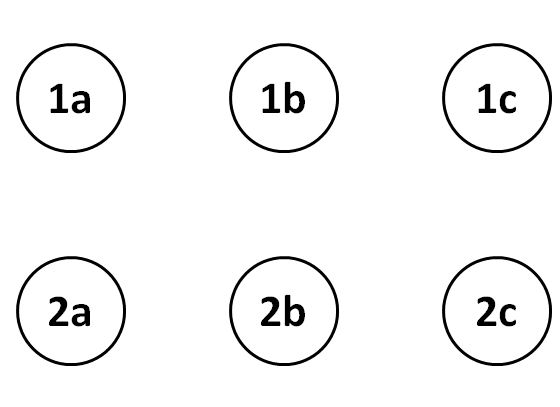
\includegraphics[width=0.4\linewidth,keepaspectratio]{bilder/bsg_ag_nodes.png}
%\caption{Die Knoten des Assoziationsgraphen von $G_1$ und $G_2$}
%\label{pic:bsg_ag_nodes}
%\end{figure}

\begin{figure}[htb]
\centering
\vspace{0.5cm}
\begin{tikzpicture}
  [normalN/.style={circle,draw,minimum size=0.8cm,thick},
   node distance=0.8cm]

  \node[normalN] (1a) {1a};
  \node[normalN] (1b) [right=of 1a] {1b}; 
  \node[normalN] (1c) [right=of 1b] {1b};
  \node[normalN] (2a) [below=of 1a] {2a};
  \node[normalN] (2b) [below=of 1b] {2b};
  \node[normalN] (2c) [below=of 1c] {2c};
\end{tikzpicture}
\caption{Die Knoten des Assoziationsgraphen von $G_1$ und $G_2$}
\label{pic:bsg_ag_nodes}
\end{figure}

Die Kanten des AGs (dargestellt in Abbildung \ref{pic:bsg_ag_edges}) geben an, 
ob Knotenpaare (also die Zuordnung eines Knotens zu einem anderen) einander 
ausschließen. Es gibt zwei Fälle, in denen das der Fall ist: 
\begin{itemize}
  \item Ein Knoten $u$ aus $G_1$ kann nur höchstens einmal auf einen anderen 
	      Knoten in $G_2$ abgebildet werden. Alle anderen Knotenpaare, die den 
        Knoten $u$ beinhalten, sind somit nicht mehr möglich. Analog verhalten 
        sich die Knoten aus $G_2$. Sie können nur einmal Ziel einer Zuordnung 
        sein.
        
        Die so erzeugten Kanten sind in Abbildung \ref{pic:bsg_ag_edges} 
        \emph{schwarz} dargestellt.
        
  \item Hat man ein Knotenpaar, so schließt dies weitere Paare 
        aus. Diese Paare ergeben sich durch die Betrachtung der Kanten der beiden 
        ursprünglichen Graphen. Ein Paar $(u_1, u_2)$ schließt ein Paar 
        $(v_1, v_2)$ aus, wenn es eine Kante (in $G_1$) zwischen $u_1$ 
        und $v_1$ gibt, jedoch keine (in $G_2$) zwischen $u_2$ und $v_2$. 
        Dies ist nötig, da ein induzierter Teilgraph dargestellt werden soll.
        
        Die so erzeugten Kanten sind in Abbildung \ref{pic:bsg_ag_edges} 
        \emph{rot} dargestellt.

\end{itemize}

%\begin{figure}[htb]
%\centering
%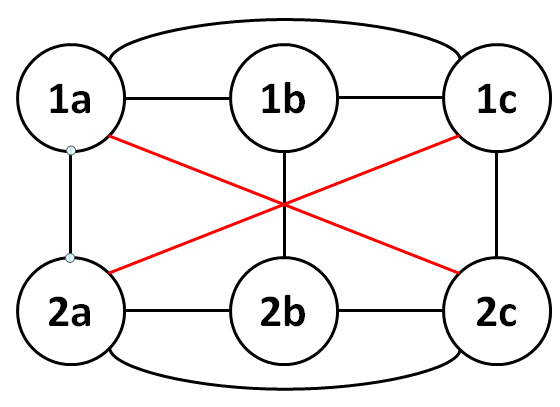
\includegraphics[width=0.4\linewidth,keepaspectratio]{bilder/bsg_ag_edges.png}
%\caption{Der vollständige Assoziationsgraphen von $G_1$ und $G_2$}
%\label{pic:bsg_ag_edges}
%\end{figure}

\begin{figure}[htb]
\centering
\begin{tikzpicture}
  [normalN/.style={circle,draw,minimum size=0.8cm,thick},
   node distance=0.8cm]

  \node[normalN] (1a) {1a};
    
  \node[normalN] (1b) [right=of 1a] {1b}
     edge [thick] (1a); 
    
  \node[normalN] (1c) [right=of 1b] {1c}
     edge [thick] (1b);
    
  \node[normalN] (2a) [below=of 1a] {2a}
     edge [thick] (1a);
    
  \node[normalN] (2b) [below=of 1b] {2b}
     edge [thick] (1b)
     edge [thick] (2a);
    
  \node[normalN] (2c) [below=of 1c] {2c}
     edge [thick] (1c)
     edge [thick] (2b);
  
  \draw [thick,red] (1a) to (2c);
  \draw [thick,red] (2a) to (1c);
  
  \draw [thick] (1c) .. controls +(135:1.3cm) and +(45:1.3cm) .. (1a);
  \draw [thick] (2c) .. controls +(-135:1.3cm) and +(-45:1.3cm) .. (2a);
\end{tikzpicture}
\caption{Der vollständige Assoziationsgraph von $G_1$ und $G_2$}
\label{pic:bsg_ag_edges}
\end{figure}

Für einen AG ergibt sich somit die folgende (auf der Beschreibung in 
\cite{MaxCSwitMaxIS} basierende) Definition:

\begin{mydef}[Assoziationsgraph]\label{def:Assoziationsgraph}
Gegeben seinen zwei Graphen $G_1=(V_1,E_1)$ und $G_2=(V_2,E_2)$. Ein 
Assoziationsgraph $G_A(G_1,G_2)=(V_A,E_A)$ sei wie folgt definiert:
\begin{itemize}
	\item $V_A= V_1 \times V_2$
	\item $E_A=\{((u_1,u_2),(v_1,v_2))\ |\ u_i=v_i \vee 
	       ((u_1,v_1) \in E_1 \oplus  (u_2,v_2) \in E_2)\}$\footnote{$a \oplus b \equiv
	       (a \wedge \neg b) \vee (\neg a \wedge b)$ -- "`Entweder $a$ oder $b$"'}
\end{itemize}
\end{mydef}

Jedes independent set im AG von $G_1$ und $G_2$ stellt nun einen gemeinsamen 
induzierten Teilgraphen von $G_1$ und $G_2$ dar \cite{MaxCSwitMaxIS}. Somit 
entspricht das MIS des AGs dem MCS von $G_1$ und $G_2$.


\chapter{Algorithmen}

Dieses Kapitel beschäftigt sich mit verschiedenen Ansätzen, um den 
Graphabstand zu ermitteln. Im ersten Abschnitt wird versucht, einen 
gemeinsamen induzierten Teilgraphen zu finden. Es wird dabei nicht 
in den ursprünglichen Graphen gesucht sondern in deren Kantengraphen. 
Der zweite Abschnitt beschäftigt sich mit der direkten Suche nach 
einem ECGM in den ursprünglichen Graphen. Dies entspricht der Suche 
nach dem größten gemeinsamen Teilgraph, der jedoch nicht induziert 
sein muss. Algorithmen, die direkt nach einem Graphabstand suchen, 
werden im dritten Abschnitt vorgestellt. 

\section{Algorithmen für MCS}

Die Algorithmen in diesen Abschnitt suchen nach einem MCS. Dabei 
wird nicht der MCS der Originalgraphen ermittelt, sondern der 
Kantengraphen. Dies wird gemacht, weil der MCS ein induzierter 
Teilgraph ist und es passieren kann, dass Knoten ungewollt als 
fehlerhaft oder fehlend angesehen werden (siehe Abschnitt \ref{sec:MCS_Graphabstand}). 

\subsection{McGregor-Algorithmus}\label{sec:McGregor}
Der McGregor-Algorithmus ist ein einfacher Backtracking-Algorithmus. 
Er wurde 1982 erstmalig veröffentlicht und liefert eine exakte 
Lösung. Er wurde unter anderem auch in \cite{MaxCGAlgComp} 
betrachtet. 

\subsubsection{Arbeitsweise}
\begin{lstlisting}[float=htb, caption={McGregor-Algorithmus},label={lst:McGregor}]
Procedure McGregor($comSubgraph$)
    For Each $(u,v) \in V_1 \times V_2$
        If $comSubgraph$.IsAddablePair($u$,$v$) Then

            $comSubgraph$.AddPair($u$,$v$)
        
            If $comSubgraph$.PairCount $>$ $max$.PairCount Then
                $max$ = $comSubgraph$.Clone()
            End If
            
            // Gibt es in beiden Eingabegraphen Knoten, die nicht zum Teilgraphen gehören?
            If $comSubgraph$.IsExpandable Then
                McGregor($comSubgraph$)
            End If
            
            // Backtracking
            $comSubgraph$.RemovePair($u$,$v$)
        End If
    End For
End Procedure
\end{lstlisting}

Das Backtracking wird mittels Rekursion realisiert. Bei jedem 
Rekursionsaufruf ist bereits ein gemeinsamer Teilgraph vorhanden, 
wobei es sich dabei am Anfang um einen leeren Graphen handelt.

Nun werden von den noch möglichen Knotenpaaren der beiden 
Ursprungsgraphen alle durchprobiert. Dabei wird überprüft, ob es 
sich weiterhin um einen induzierten Teilgraphen handelt, wenn das 
aktuelle Knotenpaar zum bisher ermittelten Teilgrpahen hinzugefügt 
wird. Dies ist dann der Fall, wenn zwischen jedem bisherigen 
Knotenpaar $(u_i,v_i)$ sowie dem aktuellen Paar $(u,v)$ entweder in 
beiden Eingabegraphen eine Kante ist, oder in keinem der Graphen 
eine Kante ist ($(u_i,u) \in E_1 \Leftrightarrow (v_i,v) \in E_2$). 
Außerdem darf keiner der Knoten bereits für ein Knotenpaar des 
aktuellen Teilgraphen benutzt worden sein.

Erfüllt ein Knotenpaar diese Bedingungen (is addable), dann wird es zum 
aktuellen Teilgrpahen hinzugefügt. Ist der Teilgraph nun größer als der bisher 
größte, wird er gespeichert. Als nächstes wird überprüft, ob der Teilgraph 
weiterhin vergrößert werden kann. Dies ist dann der Fall, wenn es 
in beiden Eingabegraphen noch Knoten gibt, die nicht zum gemeinsamen Teilgraph 
gehören. Lässt sich der Teilgraph vergrößern (is expandable), dann erfolgt 
ein rekursiver Aufruf, wobei der aktuelle Teilgraph übergeben wird. 
Abschließend wird das aktuelle Paar wieder vom Teilgraphen entfernt, damit 
das nächste Paar überprüft werden kann.

\subsubsection{Beispiel}
Gegeben seien die Graphen in Abbildung \ref{pic:bsp_McGregor_graphs}. Für sie soll nun 
der MCS mittels McGregor-Algorithmus entwickelt werden.

%\begin{figure}[htb]
%\centering
%\hspace*{\fill}
%\subfloat[Der Graph $G_1$]{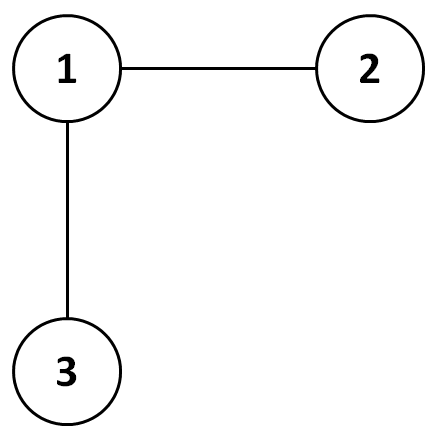
\includegraphics[width=0.3\linewidth,
%keepaspectratio]{bilder/bsp_McGregor_g1}}
%\hspace*{\fill}
%\subfloat[Der Graph $G_2$]{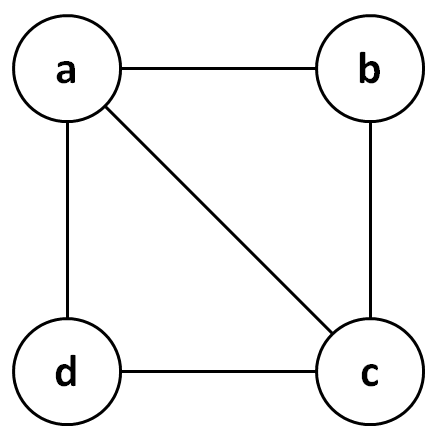
\includegraphics[width=0.3\linewidth,
%keepaspectratio]{bilder/bsp_McGregor_g2}}
%\hspace*{\fill}
%\caption{Die Graphen $G_1$ und $G_2$}
%\label{pic:bsp_McGregor_graphs}
%\end{figure}

\begin{figure}[htb]
\centering
\hspace*{\fill}
\subfloat[Der Graph $G_1$]{\begin{tikzpicture}
  [normalN/.style={circle,draw,minimum size=0.8cm,thick},
   node distance=1.3cm]

  \node[normalN] (a) {1};
    
  \node[normalN] (b) [right=of a] {2}
    edge [thick] (a);
    
  \node[normalN] (d) [below=of a] {3}
    edge [thick] (a);
  
\end{tikzpicture}}
\hspace*{\fill}
\subfloat[Der Graph $G_2$]{\begin{tikzpicture}
  [normalN/.style={circle,draw,minimum size=0.8cm,thick},
   node distance=1.3cm]

  \node[normalN] (a) {a};
    
  \node[normalN] (b) [right=of a] {b}
    edge [thick] (a);
    
  \node[normalN] (c) [below=of b] {c}
    edge [thick] (b)
    edge [thick] (a);
    
  \node[normalN] (d) [left=of c] {d}
    edge [thick] (a)
    edge [thick] (c);
  
\end{tikzpicture}}
\hspace*{\fill}
\caption{Die Graphen $G_1$ und $G_2$}
\label{pic:bsp_McGregor_graphs}
\end{figure}


Es folgt nun die Betrachtung eines einzelnen Aufrufs der McGregor-Prozedur, 
wobei schon ein Teilgraph ($comSubgraph$) vorgegeben ist. Dabei stellen \emph{rote} Linien 
Kanten in $G_1$ dar und \emph{grüne} Linien Kanten in $G_2$. Ist eine Linie 
gestrichelt, dann bedeutet dies, dass zwischen beiden Knoten keine Kante 
vorhanden ist.

Die Paare $(1,a)$ und $(2,b)$ sind bereits als Teilgraph vorgegeben. 
Als mögliche Paare aus $V_1$ und $V_2$, deren Knoten noch nicht 
verwendet wurden, bleiben noch $(3,c)$ und $(3,d)$. 
Abbildung \ref{pic:bsp_McGregor_pairs} stellt die Überprüfung dar.

%\begin{figure}[htb]
%\centering
%\hspace*{\fill}
%\subfloat[]{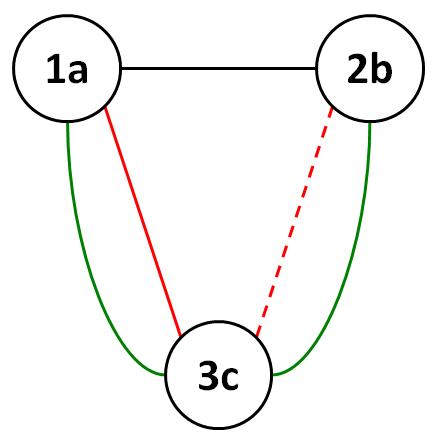
\includegraphics[width=0.3\linewidth,
%keepaspectratio]{bilder/bsp_McGregor_3c}}
%\hspace*{\fill}
%\subfloat[]{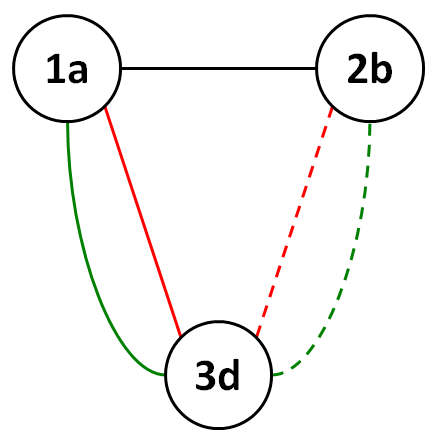
\includegraphics[width=0.3\linewidth,
%keepaspectratio]{bilder/bsp_McGregor_3d}}
%\hspace*{\fill}
%\caption{Überprüfung von Paaren}
%\label{pic:bsp_McGregor_pairs}
%\end{figure}

\begin{figure}[htb]
\centering
\hspace*{\fill}
\subfloat[]{\begin{tikzpicture}
  [normalN/.style={circle,draw,minimum size=0.8cm,thick},
   node distance=1.3cm]

  \path (0,0)     node[normalN] (l) {1a}
       +(-60:2.1) node[normalN] (b) {3c};
       
  \node[normalN] (r) [right=of l] {2b};

    
  \draw [thick] (l) -- (r);
  
  \draw [thick,red] (l) -- (b);
  \draw [thick,darkgreen,out=-90,in=180] (l) to (b);

  \draw [thick,red,dashed] (r) -- (b);
  \draw [thick,darkgreen,out=-90,in=0] (r) to (b);
    
\end{tikzpicture}}
\hspace*{\fill}
\subfloat[]{\begin{tikzpicture}
  [normalN/.style={circle,draw,minimum size=0.8cm,thick},
   node distance=1.3cm]

  \path (0,0)     node[normalN] (l) {1a}
       +(-60:2.1) node[normalN] (b) {3d};
       
  \node[normalN] (r) [right=of l] {2b};

    
  \draw [thick] (l) -- (r);
  
  \draw [thick,red] (l) -- (b);
  \draw [thick,darkgreen,out=-90,in=180] (l) to (b);

  \draw [thick,red,dashed] (r) -- (b);
  \draw [thick,dashed,darkgreen,out=-90,in=0] (r) to (b);
    
\end{tikzpicture}}
\hspace*{\fill}
\caption{Überprüfung von Paaren}
\label{pic:bsp_McGregor_pairs}
\end{figure}

Das Paar $(3,c)$ wird 
zuerst überprüft. Es kann jedoch nicht zum gemeinsamen Teilgraphen hinzugefügt 
werden, weil es eine Kante $(b,c)$ in $G_2$ gibt, jedoch keine 
Kante $(2,3)$ in $G_1$.

Als nächstes überprüft der Algorithmus das Paar $(3,d)$. Die Kanten $(1,3)$ 
und $(a,d)$ sind in $G_1$ und $G_2$ vorhanden. Außerdem sind weder $(2,3)$ 
noch $(b,d)$ in $G_1$ bzw. $G_2$ vorhanden. Somit kann $(3,d)$ zum 
Teilgraphen hinzugefügt werden. 

Nach dem Hinzufügen des Paars zum Teilgraphen, wird der neue gemeinsame 
Teilgraph mit dem bisherigen größten verglichen und gegebenenfalls gespeichert. 
Im nächsten Schritt wird überprüft, ob der Teilgraph erweitert werden kann. 
Dies ist nicht der Fall, da bereits alle Knoten aus $G_1$ verbraucht wurden. 
Zuletzt wird das Paar $(3,d)$ wieder entfernt, um andere Möglichkeiten zu probieren 
(die es in diesem Beispiel jedoch nicht gibt). 

\subsection{MIS-basierter Algorithmus}
Der folgende Algorithmus basiert auf einem Verfahren, das in \cite{MaxCSwitMaxIS} 
vorgestellt wurde. Er arbeitet mit dem Assoziationsgraphen der zu 
vergleichenden Graphen und sucht dort ein MIS (siehe Abschnitt \ref{sec:MIS_MCS}). 


\subsubsection{Arbeitweise}
\begin{lstlisting}[float=htbp,caption={MIS-basierter Algorithmus},label={lst:MIS}]
Procedure MaxIndSet($G_1$,$G_2$)

    $(V_A,E_A)$ = AssoziationsGraph($G_1$,$G_2$)
    $max$ = $\emptyset$ 
    
    // aktuelles independent set
    $selectedNodes$ = $\emptyset$
    
    // Menge der blockierten Knoten
    $blockedNodes_0$ = $\emptyset$
    
    MIS($1$)
    
End Procedure

Procedure MIS($i$)

    // Blockierung übernehmen.
    $blockedNodes_i$ = $blockedNodes_{i-1}$.Clone()
    
    // Alle unblockierten Knoten testen.
    For Each $v \in V_A \backslash blockedNodes_i$
    
        $selectedNodes$ = $selectedNodes \cup \{v\}$
        $blockedNodes_i$ = $blockedNodes_i \cup \{v\}$
    
        // Jeden Nachbarknoten von $v$ blockieren.
        For Each $(v,u) \in E_A$
            $blockedNodes_i$ = $blockedNodes_i \cup \{u\}$
        End For
        
        If $|selectedNodes| > |max|$ Then
            $max$ = $selectedNodes$
        End If
        
        MIS($i+1$)
        
        // Backtracking
        $selectedNodes$ = $selectedNodes \backslash \{v\}$
       
    End For
End Procedure
\end{lstlisting}

Im ersten Schritt baut der Algorithmus den Assoziationsgraphen für die gegebenen 
Graphen auf. Als nächstes wird im Assoziationsgraph nach einem independent set 
gesucht. Dies erfolgt über rekursiv implementiertes Backtracking. Bei jedem 
Rekursionsaufruf ist bereits ein Menge an gewählten Knoten ($selectedNodes$), 
die ein independent set darstellen, vorhanden, wobei es sich 
dabei am Anfang um eine leere Menge handelt.

Bei jedem Rekursionsaufruf wird nun nacheinander jeder Knoten $v$, der nicht zur 
Menge der blockierten Knoten ($blockedNodes$) gehört, zur aktuellen Knotenmenge 
hinzugefügt. Anschließend wird $v$ ebenfalls blockiert.

Ein Knoten wird immer dann 
blockiert, wenn er bereits zum aktuellen independent set gehört oder er nicht 
zur aktuellen Knotenmenge hinzugefügt werden kann, weil sie dann kein inependent 
set mehr ist.

Da ein independent set sich dadurch definiert, dass es keine Kanten 
besitzt, schließt die Wahl von $v$ auch alle Knoten $u$ aus, die über eine Kante 
mit $v$ verbunden sind. Auch sie werden blockiert.

Nun erfolgt der rekursive Aufruf. Abschließend wird $v$ wieder aus 
dem aktuellen independent set entfernt. Auch die Blockierungen der 
Knoten müssen wieder aufgehoben werden. In der in Listing~\ref{lst:MIS} 
dargestellten Umsetzung ist dies dadurch gelöst, dass es für jede 
Rekursionstiefe eine separate Menge von blockierten Knoten gibt. Diese 
lassen sich jeweils über einen Index ansprechen.

\subsubsection{Anpassung an einen Kantengraph}
Handelt es sich bei den gegebenen Graphen um Kantengraphen, so lässt 
sich der Assoziationsgraph $A$ vereinfachen. Jeder Knoten in $A$ 
 steht dann für eine Zuordnung eines Knotens von 
$k(G_1)$ zu einem Knoten aus $k(G_2)$. Es ist jedoch nicht möglich, 
zwei Knoten einander zuzuordnen, wenn einer der Knoten einen Knoten 
in $G_1$ darstellt und der andere eine Kante in $G_2$. Sämtliche Knoten, die 
eine solche Zuordnung darstellen, können somit aus dem Assoziationsgraph 
entfernt werden.

\subsection{Weitere Verfahren}
Es existieren noch weitere Verfahren, um einen MCS zweier Graphen zu ermitteln. 
Aufgrund der verwendeten Eigenschaften, ist jedoch vermutlich keine bessere 
Laufzeit zu erwarten.

In \cite{MCSviaVertexCover} wird ein Verfahren vorgestellt, welches mit 
dem Vertex Cover einer der Graphen arbeitet. Ein Vertex Cover eines Graphen ist 
eine Knotenmenge, bei der jede Kante des Graphen an mindestens einem 
Ende mit einem der Knoten verbunden ist. Ist ein Vertex Cover gefunden, 
wird anschließend mit dem Vertex Cover statt dem gesamten Gaphen 
weitergearbeitet. Insgesamt wird 
das ursprüngliche Problem auf drei kleinere Probleme 
aufgeteilt. Dies ist vermutlich\footnote{\cite{MCSviaVertexCover} geht nicht ausreichend 
darauf ein.} der Grund für die deutlich geringe Laufzeit gegenüber oben genannten 
Verfahren. 

Dass dieses Verfahren bei einem Kantengraph den gleichen Unterschied in der Laufzeit 
zeigt, ist nicht zu erwarten. Das minimale Vertex Cover eines Kantengraphs entspricht 
der Menge der Knoten des ursprünglichen Graphen\footnote{Dies gilt, falls der Graph 
mehr Kanten als Knoten besitzt und zusammenhängend ist. Besitzt der Graph mehr Knoten 
als Kanten, so ergibt sich das minimale Vertex Cover für den Kantengraph aus der Menge 
der Kanten. Bei nicht zusammenhängenden Graphen kann jeder zusammenhängende Teilgraph 
separat betrachtet werden.}. Die Folge ist, dass das Problem nicht aufgeteilt wird. 
Es bleibt in seiner ursprünglichen Größe vorhanden. 

\section{Direkte Suche nach einem ECGM}
Betrachtet man einen Kantengraph statt einem normalen, so bringt dies Vorteile. 
Zum einen lässt sich aus dem MCS der Kantengraphen auch ein ECGM der ursprünglichen 
Graphen ableiten. Zum anderen bietet sich die Möglichkeit, gemeinsame freie 
Kanten zu erhalten, auch wenn die dazugehörigen Knoten nicht Teil eines gemeinsamen 
Teilgraphen sind.

Angenommen, eine solche freie Kante enthält keine zusätzlichen nutzbringenden 
Informationen. In einem solchen Fall kann man direkt nach einem ECGM suchen. Die 
Algorithmen in diesem Abschnitt ermitteln ein solches ECGM. 

\subsection{Vorüberlegungen}\label{Vorueberlegungen}
Der Graphabstand zweier Graphen $G_1=(V_1,E_1)$ und $G_2=(V_2,E_2)$ ergibt sich aus 
den Kosten für das Entfernen und Hinzufügen ungleicher Elemente. Folglich ist der 
Graphabstand minimal, wenn die Menge gemeinsamer Elemente möglichst groß ist. Diese 
Menge wird durch das ECGM $\varphi:\hat{V}_1 \rightarrow \hat{V}_2$ dargestellt. 
Dabei gelte $|V_1| \leq |V_2|$. 

\begin{myTheo}\label{alleVausV1enthalten}
Gegeben seien zwei Graphen $G_1=(V_1,E_1)$ und $G_2=(V_2,E_2)$ mit 
$|V_1|\leq|V_2|$, ein ECGM $\varphi:\hat{V}_1 \rightarrow 
\hat{V}_2$ und dessen Kostenfunktion $c(\varphi)$ mit $c_{nd}(u) + c_{na}(v) > 0$ 
für alle $(u,v) \in V_1 \times V_2$. Ist $c(\varphi)$ minimal, dann ist $\hat{V}_1=V_1$.
\end{myTheo}

\begin{myProof}
Angenommen, $c(\varphi)$ sei minimal, jedoch sei $\hat{V}_1\subset V_1$. Dann
existiert ein Knoten $u \in V_1 \backslash \hat{V}_1$, sowie ein Knoten $v\in V_2
\backslash \hat{V}_2$.

Es sei nun $\lambda:\hat{V}_1 \cup \{u\} \rightarrow \hat{V}_2
\cup \{v\}$ ein weiteres ECGM. Dabei gelte:
\[
\lambda(x)=\left\{\begin{array}{ll}v & x = u \\
                                   \varphi(x) & \text{sonst}
                  \end{array}\right.
\]

Die Kosten für $\lambda$ ergeben sich nun aus den Kosten von $\varphi$, 
jedoch entfallen die Kosten für das Hinzufügen und Entfernen der Knoten 
$u$ und $v$.
\[ c(\lambda)=c(\varphi)-(c_{nd}(u)+c_{na}(v)). \]

Da $c_{nd}(u) + c_{na}(v)>0$ ist, gilt somit $c(\lambda)<c(\varphi)$. 
Somit kann $c(\varphi)$ nicht minimal sein. \qed
\end{myProof}

Satz \ref{alleVausV1enthalten} sagt aus, dass in einem ECGM 
mit minimalen Kosten 
alle Knoten des kleineren Graphen $G_1$ vorhanden sind. Ein 
ECGM lässt sich somit als Permutation der Knoten in $V_2$ 
mit der Größe $|V_1|$ darstellen: Steht ein Knoten $v$ aus $V_2$ 
an $i$-ter Position in der Permutation, wird er dem $i$-ten Knoten 
aus $V_1$ zugeordnet. Ist $v$ nicht in der Permutation vorhanden, 
dann wird ihm kein Knoten zugeordnet.

\subsubsection{Bewertung}
Die Bewertung einer Permutation erfolgt über die Kanten. Dazu werden 
die Knotenpaare $(u_1,v_1)$ aus $G_1$ mit den dazugehörigen Paaren 
$(u_2,v_2)=(\varphi(u_1),\varphi(v_1))$ aus $G_2$ verglichen. Befindet sich 
zwischen beiden Paaren eine Kante, dann wird $(u_1,v_1)$ als gleiches 
Paar mit Kante gezählt. Ist weder zwischen $(u_1,v_1)$ noch zwischen 
$(u_2,v_2)$ eine Kante, handelt es sich lediglich um ein gleiches Paar 
ohne Kante. Alle anderen Paare werden als ungleich betrachtet. 

Eine Permutation $P$ gilt als größer als eine Permutation $Q$, wenn die 
Anzahl der gleichen Paare mit Kante in $P$ größer ist als in $Q$. 
Ist die Anzahl in beiden Permutationen gleich, so ist die Anzahl der 
gleichen Paare ohne Kante entscheidend.

\subsubsection{Beispiel}
Als Beispiel seien erneut die Graphen aus Abschnitt \ref{sec:McGregor} 
gegeben (Abbildung \ref{pic:bsp_Permut_graphs}). Da $G_1$ der kleinere 
der beiden Graphen ist, wird eine dreielementige Permutation der Knoten 
aus $G_2$ gesucht. Insgesamt gibt es 24 mögliche Permutationen, von 
denen nun zwei betrachtet werden.

\begin{figure}[htb]
\centering
\hspace*{\fill}
\subfloat[Der Graph $G_1$]{\begin{tikzpicture}
  [normalN/.style={circle,draw,minimum size=0.8cm,thick},
   node distance=1.3cm]

  \node[normalN] (a) {1};
    
  \node[normalN] (b) [right=of a] {2}
    edge [thick] (a);
    
  \node[normalN] (d) [below=of a] {3}
    edge [thick] (a);
  
\end{tikzpicture}}
\hspace*{\fill}
\subfloat[Der Graph $G_2$]{\begin{tikzpicture}
  [normalN/.style={circle,draw,minimum size=0.8cm,thick},
   node distance=1.3cm]

  \node[normalN] (a) {a};
    
  \node[normalN] (b) [right=of a] {b}
    edge [thick] (a);
    
  \node[normalN] (c) [below=of b] {c}
    edge [thick] (b)
    edge [thick] (a);
    
  \node[normalN] (d) [left=of c] {d}
    edge [thick] (a)
    edge [thick] (c);
  
\end{tikzpicture}}\hspace*{\fill}
\caption{Die Graphen $G_1$ und $G_2$}
\label{pic:bsp_Permut_graphs}
\end{figure}

Die Darstellung der Permutationen erfolgt analog zu Abschnitt \ref{sec:McGregor}. 
Paare aus $G_1$ sind \emph{rot}, Paare aus $G_2$ \emph{grün}. Besitzen Paare eine 
Kante, so ist die dazugehörige Linie durchgezogen. Ist keine Kante vorhanden, dann 
ist die Linie gestrichelt.

%\begin{figure}[htb]
%\centering
%\hspace*{\fill}
%\subfloat[Permutation $P_1$\label{pic:bsp_Permut_abd}]
%         {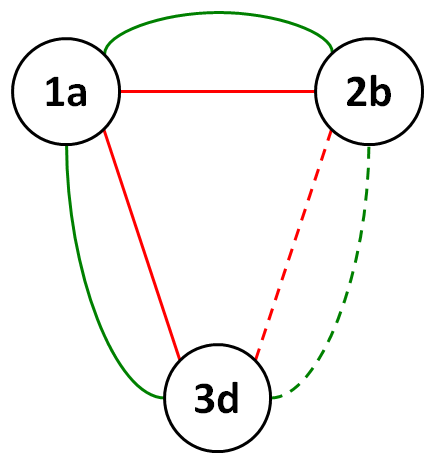
\includegraphics[width=0.3\linewidth,keepaspectratio]{bilder/bsp_Permut_abd}}
%\hspace*{\fill}
%\subfloat[Permutation $P_2$\label{pic:bsp_Permut_dbc}]
%         {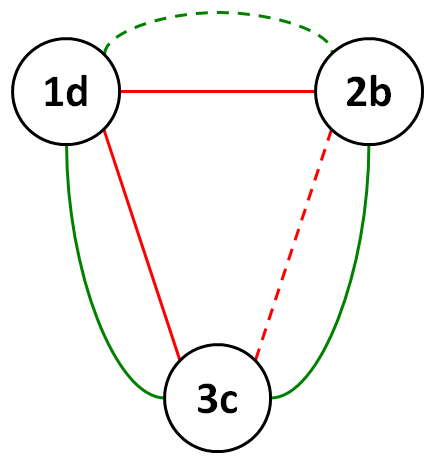
\includegraphics[width=0.3\linewidth,keepaspectratio]{bilder/bsp_Permut_dbc}}
%\hspace*{\fill}
%\caption{Überprüfung von Paaren}
%
%\end{figure}

\begin{figure}[htb]
\centering
\hspace*{\fill}
\subfloat[Permutation $P_1$\label{pic:bsp_Permut_abd}]
{\begin{tikzpicture}
  [normalN/.style={circle,draw,minimum size=0.8cm,thick},
   node distance=1.3cm]

  \path (0,0)     node[normalN] (l) {1a}
       +(-60:2.1) node[normalN] (b) {3d};
       
  \node[normalN] (r) [right=of l] {2b};

    
  \draw [thick,red] (l) -- (r);
  \draw [thick,darkgreen,out=45,in=135] (l) to (r);
  
  \draw [thick,red] (l) -- (b);
  \draw [thick,darkgreen,out=-90,in=180] (l) to (b);

  \draw [thick,red,dashed] (r) -- (b);
  \draw [thick,darkgreen,out=-90,in=0,dashed] (r) to (b);
    
\end{tikzpicture}}
\hspace*{\fill}
\subfloat[Permutation $P_2$\label{pic:bsp_Permut_dbc}]
{\begin{tikzpicture}
  [normalN/.style={circle,draw,minimum size=0.8cm,thick},
   node distance=1.3cm]

  \path (0,0)     node[normalN] (l) {1d}
       +(-60:2.1) node[normalN] (b) {3c};
       
  \node[normalN] (r) [right=of l] {2b};

    
  \draw [thick,red] (l) -- (r);
  \draw [thick,darkgreen,out=45,in=135,dashed] (l) to (r);
  
  \draw [thick,red] (l) -- (b);
  \draw [thick,darkgreen,out=-90,in=180] (l) to (b);

  \draw [thick,red,dashed] (r) -- (b);
  \draw [thick,darkgreen,out=-90,in=0] (r) to (b);
    
\end{tikzpicture}}
\hspace*{\fill}
\caption{Überprüfung von Paaren}
\end{figure}


Die Permutation $P_1=(a,b,d)$ ist in Abbildung \ref{pic:bsp_Permut_abd} dargestellt. 
Die Paare $(1,2)$, $(1,3)$, $(a,b)$ und $(a,d)$ besitzen alle eine Kante. Die Paare 
$(2,3)$ und $(b,d)$ haben beide keine Kante. Somit hat $P_1$ zwei gemeinsame Paare 
mit Kanten und ein gemeinsames Paar ohne Kante.

Die Permutation $P_2=(d,b,c)$ ist in Abbildung \ref{pic:bsp_Permut_dbc} dargestellt. 
Die Paare $(1,3)$ und $(a,c)$ besitzen beide eine Kante. Die Paare 
$(1,2)$ und $(d,b)$ sowie $(2,3)$ und $(b,c)$ haben entweder eine Kante in $G_1$ oder 
in $G_2$, jedoch nicht in beiden gleich. Somit hat $P_2$ nur ein gemeinsames Paar 
mit Kante.

\subsection{Probieren aller Permutationen}
Die einfachste Variante, die beste Permutation zu finden, ist es, alle Permutation 
zu probieren. Die Permutationen können iterativ erzeugt werden. Dabei wird eine 
Permutation direkt aus ihrem Vorgänger gebildet, bis die letzte Permutation erreicht 
ist.

\begin{lstlisting}[float=h, caption={Probieren aller Permutationen},label={lst:Permut}]
Procedure Permut($G_1$,$G_2$)
    $P$ = firstPermut($V_1$,$V_2$)
    $P_{max}$ = $P$
    Do Until isLastPermut($P$)
        If $P > P_{max}$ Then
            $P_{max}$ = $P$
        End If
        $P$ = nextPermut($P$,$V_1$,$V_2$)
    End Do
End Procedure
\end{lstlisting}

Eine Alternative zu einer iterativen Erzeugung von Permutationen ist es, alle 
Möglichkeiten rekursiv zu durchsuchen. Dadurch wird ein Suchbaum erzeugt, dessen 
Blätter eine Permutation darstellen. Ein solches Verfahren kann schneller als 
ein iteratives sein, wenn das Erzeugen einer Permutation aus einer bestehenden 
rechenaufwendig wird. Die Komplexität ändert sich jedoch nicht, denn die 
Anzahl der Permutationen (und somit die Anzahl der Blätter im Suchbaum) bleibt gleich. 

\subsection{Ein Branch-and-Bound-Verfahren}\label{BBAlgo}
Bei einem Branch-and-Bound-Verfahren (B\&B) wird ein Suchbaum aufgebaut, dessen 
Blätter eine mögliche Lösung darstellen. Die Suchstrategie innerhalb des Baums 
unterscheidet sich jedoch von einer Tiefen- oder Breitensuche. Das Verfahren wurde 
erstmals 1960 in \cite{BBOrginal} vorgestellt.

\subsubsection{Arbeitsweise}
Jeder Knoten erhält einen Wert, der eine obere bzw. untere (abhängig davon, ob ein 
Maximum oder Minimum gesucht wird) Schranke für alle Lösungen des Teilbaums angibt. 
Das bedeutet, dass keine der Lösungen in dem Teilbaum besser sein kann, als am 
aktuellen Knoten abgeschätzt wird. 
Bei der Wurzel des Baums beginnend wird der Suchbaum schrittweise an dem Knoten 
erweitert, der die beste Lösung verspricht. Ist der Knoten mit dem besten Wert ein 
Blatt, dann stellt er eine optimale Lösung dar. 

\begin{lstlisting}[float=h, caption={Prinzip des Branch-and-Bound-Algorithmus},label={lst:BB}]
Procedure BB()

    $pQ$ = New PriorityQueue()
    $pQ$.Enqueue($rootNode$)

    Do Until isLeaf($pQ$.Top())
        $top$ = $pQ$.Dequeue()

        For Each $node$ In expand($top$)
            $pQ$.Enqueue($node$)
        End For
    End Do
End Procedure
\end{lstlisting}

Der Vorteil eines B\&B-Verfahrens ist, dass nicht der gesamte Baum durchsucht werden 
muss. Aufgrund der Schranken müssen bestimmte Teilbäume nicht durchsucht werden. 
Nachteilig ist allerdings ein erhöhter Speicheraufwand. Jeder Knoten, der im 
nächsten Schritt expandiert werden kann, muss gespeichert werden. 
Ob der Vorteil oder der Nachteil überwiegt, hängt stark von der gewählten Schranke ab. 
Bildet sich eine deutliche Lösung heraus, wird der Baum nur selten erweitert. Somit 
sind Zeit- und Speicheraufwand gering. Sind alle Knoten etwa gleichwertig, muss der 
Baum häufiger erweitert werden. Im ungünstigsten Fall wird der Suchbaum fast komplett 
aufgespannt. Sowohl Zeit- wie Speicheraufwand sind dann sehr hoch. 

\subsubsection{Beispiel}

%\begin{figure}[htb]
%\centering
%\includegraphics[width=0.7\linewidth,keepaspectratio]{bilder/bsp_BnB_1.png}
%\caption{Beispiel-Suchbaum für das B\&B-Verfahren}
%\label{pic:bsp_BnB_1}
%\end{figure}
Als Beispiel sei der Suchbaum in Abbildung \ref{pic:bsp_BnB_1} gegeben. In diesem soll 
das Minimum ermittelt werden. Es wird also das Blatt mit minimalem Wert gesucht. Der Wert 
der Knoten, die keine Blätter sind, gibt an, wie hoch die Werte der entsprechenden Blätter mindestens sind. 
Dieser Wert entspricht also einer unteren Schranke.


\begin{figure}[htb]
\centering
\begin{tikzpicture}
  [normalN/.style={circle,draw,minimum size=0.8cm},
   level 1/.style={sibling distance=4cm},
   level 3/.style={sibling distance=1.6cm},
   level distance=1.3cm,thick,
   node distance=1.3cm]
   

 \node [normalN,minimum size=0.4cm] (root) {}
   child {
     node [normalN] {5} [sibling distance=7mm] child[dashed] child[dashed] child[dashed]
   }
   child {
     node [normalN] {1} [sibling distance=3.2cm]
       child {
         node [normalN] {2}
         child {node [normalN] {4}}
         child {node [normalN] {2}}
       }
       child {
         node [normalN] {3}
         child {node [normalN] {3}}
         child {node [normalN] {4}}
       }
   }
   child {
     node [normalN] {4} [sibling distance=7mm] child[dashed] child[dashed] child[dashed]
   };

\end{tikzpicture}
\caption{Beispiel-Suchbaum für das B\&B-Verfahren}
\label{pic:bsp_BnB_1}
\end{figure}

Abbildung \ref{pic:bsp_BnB} zeigt den Verlauf des Verfahrens für diesen Suchbaum. 
Die Knoten, die zurzeit betrachtet werden, sind \emph{schwarz} dargestellt. 
Der Knoten mit dem minimalen Wert ist zusätzlich \emph{grün} eingefärbt. Knoten, 
die bereits betrachtet wurden und nicht mehr im Speicher sind, sind ausgegraut.

Begonnen wird mit den Unterknoten der Wurzel: $(5)$, $(1)$ und 
$(4)$. Da $(1)$ das Minimum ist, wird an dieser Stelle erweitert. 
Dazu werden die Unterknoten zur Menge der aktuellen Knoten 
hinzugefügt und $(1)$ entfernt.

Im nächsten Schritt wird der Knoten $(2)$ erweitert. Im Speicher 
befinden sich danach die Knoten $(5)$, $(4)$, $(5)$, $(3)$ und 
$(4)$. 

Zuletzt wird der Knoten $(3)$ erweitert, wodurch dieser entfernt 
wird und die Knoten $(3)$ und $(4)$ hinzugefügt werden. Das 
Minimum ist somit erneut $(3)$. Da es sich dabei um ein Blatt 
handelt, ist dieser Knoten auch ein Minimum. Die Suche wird somit 
beendet.

\begin{figure}[bht]
\centering

\subfloat[\label{pic:bsp_BnB_2}]{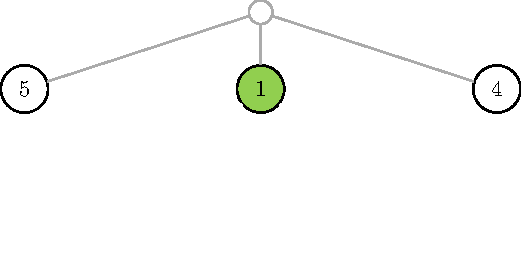
\includegraphics[width=0.45\linewidth,
keepaspectratio]{bilder/bsp_BnB_2}}
\hspace*{\fill} 
\subfloat[\label{pic:bsp_BnB_3}]{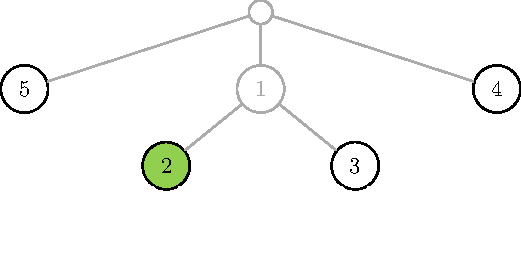
\includegraphics[width=0.45\linewidth,
keepaspectratio]{bilder/bsp_BnB_3}}

\subfloat[\label{pic:bsp_BnB_4}]{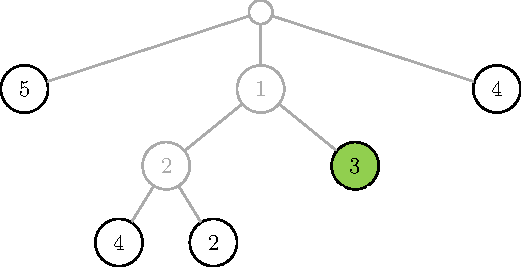
\includegraphics[width=0.45\linewidth,
keepaspectratio]{bilder/bsp_BnB_4}}
\hspace*{\fill} 
\subfloat[\label{pic:bsp_BnB_5}]{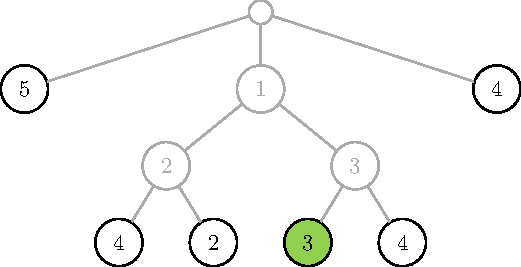
\includegraphics[width=0.45\linewidth,
keepaspectratio]{bilder/bsp_BnB_5}} 

\caption{Suche mittels B\&B-Verfahren}
\label{pic:bsp_BnB}
\end{figure}


\subsubsection{Ermitteln des ECGMs}
Jeder Knoten des Suchbaums beschreibt eine ECGM bzw. einen gemeinsamen 
Teilgraphen der Graphen $G_1$ und $G_2$. Der Wurzelknoten stellt einen 
leeren Graphen dar. Dessen Unterknoten entsprechen einem Graphen mit 
einem Knoten. Sie geben an, worauf der erste Knoten aus $G_1$ 
abgebildet wird. Die Blätter des Suchbaums geben dann einen Teilgraphen 
an, bei dem jeder Knoten aus $G_1$ enthalten ist. 

Ist ein Knoten kein Blatt, ist der durch ihn dargestellte Teilgraph 
somit kleiner als $G_1$. Folglich gibt es in beiden Graphen Knoten, 
die noch nicht einander zugeordnet wurden, also auch mögliche Paare, 
die nicht bewertet wurden. Die Anzahl der Paare mit Kanten und die 
Anzahl der Paare ohne Kanten beider Graphen werden nun miteinander 
verglichen. Die jeweils kleinere Zahl ist somit die maximale Anzahl 
an möglichen gemiensamen Paaren.
Es wird also angenommen, dass es zu jedem Paar mit oder 
ohne Kante im unbetrachteten Teil von $G_1$ auch ein Paar mit oder 
ohne Kante im unbetrachteten Teil von $G_2$ gibt. Zusammen mit der 
Anzahl der gleichen Paare im betrachteten Teil bildet dies die 
Schranke. Beim Vergleich zweier Schranken sind in erster Linie die 
Paare mit Kante entscheidend. Ist ihre Zahl gleich, werden 
zusätzlich Paare ohne Kante betrachtet. 

\subsubsection{Beispiel}
Gegeben seien die Graphen $G_1$ und $G_2$ (Abbildung~\ref{pic:bsp_BB_Bound}). 
Angenommen bei der Suche nach einem ECGM mittels B\&B-Verfahrens 
seien bereits die Zuweisungen $(1,a)$ und $(2,b)$ gegeben (grün dargestellt). 
Es soll nun ermittelt werden, wie viele gemeinsame Paare (mit oder ohne Kante) 
es maximal gibt. Paare ohne Kante sind durch gestrichelte Linien dargestellt.
%\begin{figure}[htb]
%\centering
%\hspace*{\fill}
%\subfloat[Der Graph $G_1$]{\begin{tikzpicture}
%  [normalN/.style={circle,draw,minimum size=0.8cm,thick},
%   node distance=1.3cm]
%
%  \node[normalN] (a) {1};
%    
%  \node[normalN] (b) [left=of a] {3}
%    edge [thick] (a);
%    
%  \node[normalN] (c) [below=of a] {2}
%    edge [thick] (a);
%  
%  \node[normalN] (d) [left=of c] {4}
%    edge [thick] (c);
%    
%\end{tikzpicture}}
%\hspace*{\fill}
%\subfloat[Der Graph $G_2$]{\begin{tikzpicture}
%  [normalN/.style={circle,draw,minimum size=0.8cm,thick},
%   node distance=1.3cm]
%
%  \node[normalN] (a) {a};
%    
%  \node[normalN] (b) [below=of a] {b}
%    edge [thick] (a);
%    
%  \node[normalN] (c) [right=of b] {c}
%    edge [thick] (b)
%    edge [thick] (a);
%    
%  \node[normalN] (d) [above=of c] {d}
%    edge [thick] (a)
%    edge [thick] (c);
%  
%\end{tikzpicture}}
%\hspace*{\fill}
%\caption{Die Graphen $G_1$ und $G_2$}
%\label{pic:bsp_BB_Bound_1}
%\end{figure}

\begin{figure}[htb]
\centering
\hspace*{\fill}
\subfloat[Der Graph $G_1$]{\begin{tikzpicture}
  [normalN/.style={circle,draw,minimum size=0.8cm,thick},
   node distance=1.3cm]

  \node[normalN,draw=darkgreen] (1a) {1a};
    
  \node[normalN,draw=darkgreen] (2b) [below=of a] {2b}
    edge [darkgreen,thick] (1a);
    
  \node [normalN] (3) [left=of 1a] {3}
    edge [thick] (1a)
    edge [dashed] (2b);
    
  \node [normalN] (4) [left=of 2b] {4}
    edge [dashed] (1a)
    edge [thick] (2b)
    edge [dashed] (3);
    
\end{tikzpicture}}
\hspace*{\fill}
\subfloat[Der Graph $G_2$]{\begin{tikzpicture}
  [normalN/.style={circle,draw,minimum size=0.8cm,thick},
   node distance=1.3cm]

  \node[normalN,draw=darkgreen] (1a) {1a};
    
  \node[normalN,draw=darkgreen] (2b) [below=of a] {2b}
    edge [thick,darkgreen] (1a);
    
  \node[normalN] (c) [right=of 2b] {c}
    edge [thick] (2b)
    edge [thick] (1a);
    
  \node[normalN] (d) [above=of c] {d}
    edge [thick] (1a)
    edge [dashed] (2b)
    edge [thick] (c);
    
\end{tikzpicture}}
\hspace*{\fill}
\caption{Die Graphen $G_1$ und $G_2$ mit einem gemeinsamen Knotenpaar}
\label{pic:bsp_BB_Bound}
\end{figure}

Der Graph $G_1$ besitzt zwei Paare mit Kante: $(1a,3)$ und $(2b,4)$. Außerdem 
besitzt er drei Paare ohne Kante: $(1a,4)$, $(2b,3)$ und $(3,4)$. 
$G_2$ hingegen besitzt vier Paare mit Kante ($(1a,d)$, $(1a,c)$, $(2b,c)$ 
und $(c,d)$) sowie ein Paar ohne Kante ($(2b,d)$). Von beiden Varianten 
(mit und ohne Kante) wird nun das kleinere genommen, also zwei Paare mit 
und ein Paar ohne Kante. Somit ergibt sich (nach hinzurechnen des bereits 
vorhanden Paares $(1a,2b)$) als obere Schranke: drei Paare mit 
und ein Paar ohne Kante. Bei keiner Kombination der Knoten ist mehr möglich.


\subsection{Ein evolutionärer Algorithmus}
Evolutionäre Algorithmen basieren auf dem Prinzip der biologischen 
Evolution. Dazu betrachtet man eine Population möglicher Lösungen. 
Jede Lösung ist ein Individuum, welches einen Wert besitzt, 
der die Qualität der Lösung beschreibt. Es gibt drei Mechanismen für die Suche nach 
einer besseren Lösung: Selektion, Rekombination und Mutation. 

Selektion ist schlicht eine Auswahl der qualitativ besten Lösungen. Zu 
schlechte Lösungen werden aus der Population entfernt. Sie "`sterben"'. 
Mutiert ein Individuum, wird es leicht (zufällig) geändert. Bei der 
Rekombination zweier Individuen wird ein neues Individuum auf Basis der 
beiden bestehenden erzeugt. Das Neue übernimmt dabei die Eigenschaften, 
die beide Eltern gemeinsam hatten. Alle drei Mechanismen werden nun 
nacheinander ausgeführt, bis eine Abbruchbedingung erfüllt ist.

\begin{lstlisting}[float=h, caption={Prinzip eines evolutionären Algorithmus},label={lst:Evo}]
Procedure Evolution()
    initialisiere $P$
    Do Until $Abbruchbedingung$
        Rekombination($P$)
        Mutation($P$)
        Selektion($P$)
    End Do
End Procedure
\end{lstlisting}

Der Vorteil eines evolutionären Algorithmus ist, dass man kaum Wissen 
über das zu lösende Problem benötigt. Kann man eine mögliche Lösung 
bewerten und weitere mögliche Lösungen erzeugen, dann lässt sich 
auch ein evolutionärer Algorithmus implementieren. Erfahrungsgemäß erzeugen 
evolutionäre Algorithmen dabei eine gute Lösung. Für das Finden eines 
guten ECGMs werden lediglich Permutationen betrachtet. Zwar ist für 
die Bewertung jeder Permutation wichtig, wie die dazugehörigen Graphen 
aufgebaut sind, aber für Mutation und Rekombination wird lediglich die 
Permutation betrachtet. Es findet kein Bezug zu den Graphen mehr statt.

Der Nachteil eines evolutionären Algorithmus ist jedoch, dass er kein 
exaktes Verfahren ist. Es lässt sich keine Aussage über die Qualität 
einer Lösung treffen. Bei einem endlichen Lösungsraum lässt sich eine 
Mindestwahrscheinlichkeit dafür angeben, dass die optimale Lösung 
gefunden wurde. Es ist jedoch im Allgemeinen nicht möglich zu sagen, 
ob eine Lösung ein Optimum ist oder wie weit sie vom Optimum höchstens 
entfernt ist. 

\subsubsection{Individuen}
Ein Individuum stellt eine mögliche Lösung dar. Für die Suche nach einem ECGM zweier 
Graphen kann also eine Permutation der Knoten als Individuum betrachtet werden. Als 
Bewertung für die Selektion dient erneut die Anzahl der gleichen Paare. 

\subsubsection{Umsetzung der Mutation}
Eine Mutation stellt eine kleine Veränderung des Individuums dar. Um eine Permutation 
zu mutieren, werden in der hier verwendeten Implementation lediglich die Abbildungen 
zweier zufälliger Knoten vertauscht. 

\subsubsection{Umsetzung der Rekombination}
Bei der Rekombination zweier Permutationen werden gleiche Abbildungen übernommen. 
Alle anderen Abbildungen werden zufällig verteilt. Dadurch ist es bei Graphen 
unterschiedlicher Größe möglich, auch Knoten des größeren Graphen zur Lösungsmenge 
hinzuzufügen, die bisher nicht zum gemeinsamen Teilgraph gehörten.

\section{Graphabstand-Algorithmen}
Die Algorithmen in diesem Abschnitt werden in \cite{phdRiesen} als Algorithmen zur 
Ermittlung des Graphabstands beschrieben.

\subsection{Der A*-Algorithmus}
Der A*-Algorithmus ist ursprünglich zur Pfadsuche in Graphen gedacht. Er wurde 1968 
in \cite{AStarAlg} vorgestellt. 1972 erfolgte eine leichte Korrektur in 
\cite{AStarAlgCorrection}. "`Auf dem A*-Algorithmus basiert eine weit verbreitete 
Methode"' \cite{phdRiesen} zur Berechnung des exakten Graphabstands.

\subsubsection{Arbeitsweise}
Bei einer Pfadsuche beginnt der A*-Algorithmus am Startpunkt des Graphen. Dieser wird als bekannt
markiert. Für jeden bekannten Knoten gibt es eine Menge möglicher unmarkierter
Folgeknoten, die über eine Kante erreichbar sind. Der Folgeknoten, der den
kürzesten Pfad zum Ziel verspricht, wird als nächstes markiert. Dies wiederholt sich
so lange bis der Zielknoten erreicht ist.

Um zu entscheiden, welcher Knoten $v$ als nächstes markiert wird, gibt es zu jedem eine 
Abschätzung $f(v)=g(v)+h(v)$. Dabei gibt $g(v)$ die (bekannten) minimalen Kosten zum 
Erreichen von $v$ an. Eine Abschätzung für die noch entstehenden Kosten gibt $h(v)$ an. 
Gewählt wird dann der Knoten, dessen $f(v)$ am kleinsten ist. 
Wichtig ist, dass $h(v)$ die minimalen Kosten angibt. Werden die Kosten höher 
angegeben als sie wirklich sind, kann dies zur Folge haben, dass der kürzeste Pfad nicht 
erkannt wird. 

%\begin{figure}[htb]
%\centering
%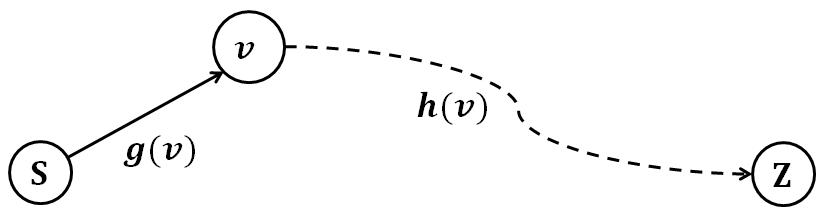
\includegraphics[width=0.9\linewidth,keepaspectratio]{bilder/aStern}
%\caption{Prinzip des A*-Algorithmus}
%\label{pic:AStern}
%\end{figure}

\begin{figure}[htb]
\vspace*{0.5cm}
\centering
\begin{tikzpicture}
  [normalN/.style={circle,draw,minimum size=0.8cm},
   thick,auto,
   node distance=1.3cm]
   
  \node at (0,0)   [normalN] (start) {S};
  \node at (2,1.2) [normalN] (v)     {v};
  \node at (6,0)   [normalN] (ziel)  {Z};

  \draw [->] (start) to node [swap] {$g(v)$} (v);
  \draw [->,out=0,in=180,dashed] (v) to node [swap] {$h(v)$} (ziel);
\end{tikzpicture}
\caption{Prinzip des A*-Algorithmus}
\label{pic:AStern}
\end{figure}


Der A*-Algorithmus kann beispielsweise verwendet werden, um in einem Straßennetz die 
kürzeste Strecke zwischen zwei Städten zu finden. Die Funktion $g(v)$ gibt dabei die 
Strecke an, die tatsächlich gefahren werden muss, um eine Stadt zu erreichen. Als 
Abschätzung für $h(v)$ kann die Luftlinie zwischen zwei Städten benutzt werden, denn 
die direkte Verbindung ist immer kürzer als die tatsächliche Straßenlänge. 

\subsubsection{Anpassung an Graphabstand}
Zur Ermittlung des Graphabstands zweier Graphen $G_1$ und $G_2$ muss der 
Algorithmus leicht angepasst werden. Der Graph, in dem ein Pfad gesucht 
wird, ist der Suchbaum zur Ermittlung eines ECGMs. 
Startknoten ist die Wurzel des Baums. Zielknoten sind die Blätter. Der Wurzelknoten 
stellt ein "`leeres"' ECGM dar. Seine Unterknoten entsprechen nun allen möglichen 
Abbildungen des ersten Knotens aus $G_1$. Dazu gehört auch das Löschen des 
Knotens. \footnote{Aufgrund von Satz \ref{alleVausV1enthalten} (Abschnitt 
\ref{Vorueberlegungen}) ist es nicht nötig, das Löschen des Knotens zu betrachten, wenn 
$G_1$ der kleinere der beiden Graphen ist. Es werden dann sämtliche Knoten aus $G_1$ 
übernommen.} 

Aus dem Teil-ECGM, das durch einen Knoten $v$ des Suchbaums 
dargestellt wird, berechnen sich die bisherigen Kosten $g(v)$. 
In der in \cite{phdRiesen} vorgestellten Variante  ergeben sie 
sich aus den Kosten für das Hinzufügen und Entfernen von Kanten. Die noch anfallenden 
Kosten $h(v)$ berechnen sich aus dem Vergleich der Kanten, die noch nicht im aktuellen 
Teil-ECGM sind. Dabei wird ermittelt, wie viele Kanten mindestens entfernt bzw. hinzugefügt
werden müssen.

\subsubsection{Vergleich mit Branch-and-Bound}
Vergleicht man den A*- mit dem B\&B-Algorithmus, stellt man 
eine starke Ähnlichkeit fest. Beide Verfahren benutzen die 
gleiche Strategie: In einem zu durchsuchenden Graphen (bei 
B\&B immer ein Suchbaum) werden die bisher erreichten Knoten 
miteinander verglichen. An dem Knoten, dessen Summe aus den 
exakten und den erwarteten Kosten minimal ist, wird die 
Suche fortgesetzt. Der A*-Algorithmus ist dabei lediglich 
für eine Minimierung gedacht. Der B\&B-Algorithmus ist etwas 
allgemeiner formuliert. Es ist auch für eine Maximierung 
ausgelegt. Dies ist jedoch kein relevanter Unterschied. Beim 
B\&B-Algorithmus lassen sich Minimierung und Maximierung 
ineinander umwandeln, indem man die Kosten bzw. die Werte 
mit $-1$ multipliziert. 

Die in \cite{phdRiesen} beschriebene Methode zur Berechnung einer unteren Schranke 
für den Graphabstad zweier Graphen basiert auf dem gleichen Prinzip wie 
die Berechnung der Schranke in Abschnitt \ref{BBAlgo}. Es wird die Anzahl der 
verbliebenen Kanten im unbetrachteten Teil der Graphen miteinander verglichen. 
Das oben vorgestellte B\&B-Verfahren ermittelt dabei die Anzahl der gemeinsamen 
Kanten. Die in \cite{phdRiesen} vorgestellte Variante zur Berechnung einer unteren 
Schranke (der noch anfallenden Kosten $h(v)$) berechnet die Zahl der zu löschenden 
Kanten. Addiert man beides, erhält man somit die Gesamtzahl der Kanten. Da diese 
für ein Graphenpaar konstant ist, sind auch beide Schranken äquivalent zueinander. 
Aus diesem Grund wird in Kapitel \ref{chp:AlgoTest} lediglich der B\&B-Algorithmus
betrachtet.

\subsection{Bipartite Heuristik}
Eine mögliche Variante, um den Graphabstand zweier Graphen abzuschätzen, ist ein 
Matching auf einem bipatiten Graphen.


\subsubsection{Grundlagen}
Ein bipartiter Graph zeichnet sich dadurch aus, dass sich dessen Knotenmenge 
in zwei Teilmengen unterteilen lässt, wobei Kanten immer jeweils einen Knoten 
der einen mit einem Knoten der anderen Teilmenge verbinden. Zwischen den Knoten 
innerhalb einer Teilmenge gibt es keine Kanten.

\begin{mydef}[bipartiter Graph]
Ein gewichteter bipartiter Graph $G$ ist ein 3-Tupel $G=(V,E,\omega)$. Dabei sind:
\begin{itemize}
	\item $V=V_1 \cup V_2$ mit $V_1 \cap V_2=\emptyset$ eine endliche Menge an Knoten,
	\item $E \subseteq V_1 \times V_2$ die Menge der Kanten und
	\item $\omega:E \rightarrow \mathbb{Q}$ die Gewichtsfunktion der Kanten.
\end{itemize}
$G$ ist \emph{voll} genau dann, wenn $E=V_1\times V_2$.
\end{mydef}

Bei einem Matching in einem Graphen werden Knoten einander zugeordnet. Dabei müssen 
die Knoten über eine Kante miteinander verbunden sein. Diese Zuordnung ist eindeutig. 
Es wird also jedem Knoten nur maximal ein anderer Knoten zugeordnet.

\begin{mydef}[Matching]
Ein Matching in einem gewichtetem bipartiten Graphen $G=(V_1 \cup V_2,E,\omega)$ ist eine bijektive
Abbildung $\mu:\hat{V_1} \rightarrow \hat{V_2}$ mit $\hat{V_1} \subseteq V_1$ und $\hat{V_2}
 \subseteq V_2$. Dabei gilt: $v \in \hat{V_1} \Rightarrow (v,\mu(v)) \in E$.
\end{mydef}

Das Gewicht $w$ eines Matchings ist dann: 
\[ w=\sum_{v \in \hat{V_1}} \omega((v,\mu(v)))  \]

\subsubsection{Arbeitsweise}
Idee der Heuristik ist, dass man ein ECGM auch als Matching in einem bipartiten Graphen
interpretieren kann. Gegeben seien die Graphen $G_1=(V_1,E_1)$ und $G_2=(V_2,E_2)$
mit $n=|V_1|$ und $m=|V_2|$. Daraus lässt sich nun
ein voller bipartiter Graph $M=(V_M,E_M,\omega)$ wie folgt erstellen:
\begin{itemize}
	\item $V_M=(V_1 \cup \{\varepsilon_{1_1},\ \ldots\ , \varepsilon_{1_m}\}) \cup
	           (V_2 \cup \{\varepsilon_{2_1},\ \ldots\ , \varepsilon_{2_n}\})$
	\item $E_M=(V_1 \cup \{\varepsilon_{1_1},\ \ldots\ , \varepsilon_{1_m}\}) \times
	           (V_2 \cup \{\varepsilon_{2_1},\ \ldots\ , \varepsilon_{2_n}\})$
\end{itemize}
Der eine Teil der Knoten in $M$ ergibt sich aus den Knoten in $G_1$ sowie 
je einem $\varepsilon$-Knoten für jeden Knoten in $G_2$. Der zweite Teil 
bildet sich analog: es werden die Knoten aus $G_2$ genommen, sowie je ein 
$\varepsilon$-Knoten für jeden Knoten in $G_1$.

Die $\varepsilon$-Knoten dienen dazu, um das Hinzufügen oder Entfernen von Knoten 
ebenfalls als Matching zu ermöglichen. Wird ein Knoten hinzugefügt, so wird ihm ein 
$\varepsilon$-Knoten zugeodnet: $\varepsilon_{1_i} \mapsto v_i$. Beim Löschen 
ist es andersrum: $v_i \mapsto \varepsilon_{2_i}$.

 Ein ECGM ist nun äquvalent zu einem Matching in $M$. 
Die Kosten $c_{u v}$, die mindestens entstehen, wenn zwei Knoten $u$ und $v$ einander 
zugewiesen werden, ergeben dann die Kantengewichte von $M$. Zur Berechnung der Kosten 
werden die Kanten von $G_1$ und $G_2$ 
mit einbezogen. Hat beispielsweise ein Knoten drei Kanten und wird auf einen Knoten mit 
fünf Kanten abgebildet, so müssen mindestens zwei Kanten entfernt oder hinzugefügt werden. 
Die Kosten können als Kosten-Matrix $C$ dargestellt werden. 

\[
C=\left [
\begin{array}{ccc|ccc}
c_{11} & \cdots & c_{1 m} & c_{1\varepsilon} &        & \infty \\
\vdots & \ddots & \vdots &                  & \ddots & \\
c_{n 1} & \cdots & c_{n m} & \infty           &        & c_{n\varepsilon} \\

\cline{1-6}

c_{\varepsilon 1} &        & \infty            & &   & \\
                  & \ddots &                   & & 0 & \\
\infty            &        & c_{\varepsilon m} & &   &

\end{array} \right ]
\]

Die Matrix ist in vier Bereiche unterteilt. Oben links befinden sich die Kosten, 
die beim Zuweisen eines Knoten aus $G_1$ zu einem Knoten aus $G_2$ auftreten. Oben 
rechts und unten links sind die Kosten für das Hinzufügen oder Löschen von Knoten. 
Die Kosten stehen jedoch nur in den Diagonalen. Alle anderen Werte sind unendlich. 
Im unteren rechten Teil sind alle Werte null. Sie stellen den Fall dar, dass zwei 
$\varepsilon$-Knoten einander zugewiesen werden.

Um nun ein ECGM zu finden, das möglichst geringe Kosten hat, wird das Matching gesucht, 
dessen Gewicht minimal ist. Dieses lässt sich durch ein Verfahren ermitteln, welches als 
Ungarische Methode\footnote{Es ist auch unter Munkres Algorithmus oder 
Kuhn-Munkres-Algorithmus bekannt.} bekannt ist. Die Methode findet ein minimales Matching 
in $\mO(n^3)$ \cite{Munkres1957}. 

\subsubsection{Matching als untere Schranke}
In \cite{RiesenSpeedingup} wird die Heuristik als mögliche Abschätzung für die 
mindestens noch entstehenden Kosten ($h$-Funktion) und somit als untere 
Schranke zur Berechnung des Graphabstands mittels eines A*-""Algorithmus vorgeschlagen. 
Die Argumentation dabei ist, dass 
die Kantengewichte des bipartiten Graphen jeweils die minimalen Kosten 
für das Abbilden der Knoten aufeinander darstellen. Somit sei das minimale 
Gesamtgewicht eines Matchings auch die minimalen Kosten für den gesamten 
Graph. Bewiesen wird diese Behauptung nicht. 
Bei einer genauen Betrachtung stellt sich diese Aussage hingegen als inkorrekt heraus. 
 Es kann passieren, dass Kosten für Kanten doppelt 
berechnet werden. Dies liegt daran, dass die Kosten an beiden Knoten der Kante 
erhoben werden.

%\begin{figure}[htb]
%\centering
%\hspace*{\fill}
%\subfloat[\label{pic:bspBipMatching1}]{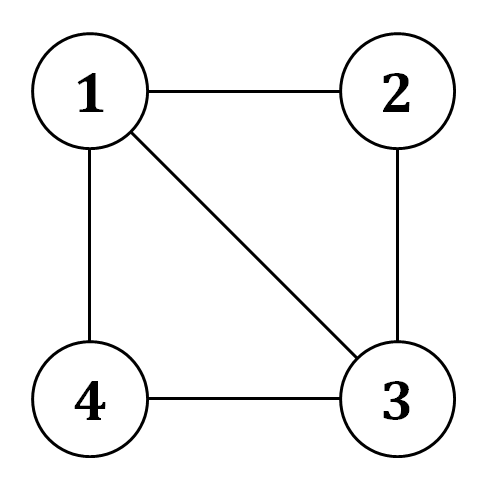
\includegraphics[width=0.3\linewidth,
%keepaspectratio]{bilder/bspBipMatching1}}
%\hspace*{\fill}
%\subfloat[\label{pic:bspBipMatching2}]{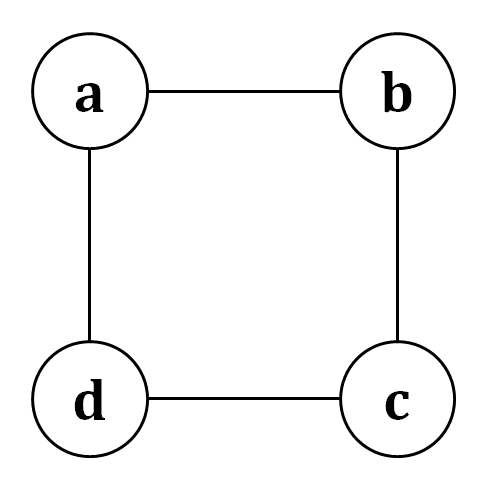
\includegraphics[width=0.3\linewidth,
%keepaspectratio]{bilder/bspBipMatching2}}
%\hspace*{\fill}
%\caption{Graphen, die sich durch genau eine Kante unterscheiden}
%\label{pic:BspBipMatching}
%\end{figure}

\begin{figure}[htb]
\centering
\hspace*{\fill}
\subfloat[\label{pic:bspBipMatching1}]{\begin{tikzpicture}
  [normalN/.style={circle,draw,minimum size=0.8cm,thick},
   node distance=1.3cm]

  \node[normalN] (a) {1};
    
  \node[normalN] (b) [right=of a] {2}
    edge [thick] (a);
    
  \node[normalN] (c) [below=of b] {3}
    edge [thick] (b)
    edge [thick] (a);
    
  \node[normalN] (d) [left=of c] {4}
    edge [thick] (a)
    edge [thick] (c);
  
\end{tikzpicture}}
\hspace*{\fill}
\subfloat[\label{pic:bspBipMatching2}]{\begin{tikzpicture}
  [normalN/.style={circle,draw,minimum size=0.8cm,thick},
   node distance=1.3cm]

  \node[normalN] (a) {a};
    
  \node[normalN] (b) [right=of a] {b}
    edge [thick] (a);
    
  \node[normalN] (c) [below=of b] {c}
    edge [thick] (b);
    
  \node[normalN] (d) [left=of c] {d}
    edge [thick] (a)
    edge [thick] (c);
  
\end{tikzpicture}}
\hspace*{\fill}
\caption{Graphen, die sich durch genau eine Kante unterscheiden}
\label{pic:BspBipMatching}
\end{figure}

Die in Abbildung \ref{pic:BspBipMatching} dargestellen Graphen sind bis auf die Kante 
in der Mitte gleich. Der Graphabstand entspricht somit lediglich dem Hinzufügen oder Entfernen 
der Kante. Die Kosten werden allerding zweimal in die Kostenmatrix übernommen und 
auch zweimal in das Gesamtgewicht des Matchings eingerechnet. 

Setzt man die Kosten für das Einfügen und Löschen von Knoten und Kanten jeweils auf $1$,
so ergibt sich folgende Kostenmatrix $C$:

\[
C=\left [
\begin{array}{cccc|cccc}
    1 & 1 & 1 & 1 & 3 &   &   & \infty \\
    0 & 0 & 0 & 0 &  & 2 &   &  \\
    1 & 1 & 1 & 1 &   &   & 3 &  \\
    0 & 0 & 0 & 0 &  \infty &   &   & 2 \\
 \cline{1-8}
         2 &   &   & \infty & \multicolumn{4}{c}{\multirow{4}{*}{0}}\\
           & 2 &   &  \\
           &   & 2 &  \\
    \infty &   &   & 2 \\

\end{array} \right ] 
\]

Ein minimales Matching ergibt sich nun aus folgenden Abbildungen:
%\begin{align*}
\[
\begin{array}{ccc}
	1 & \longmapsto & a \\
  2 & \longmapsto & b \\
  3 & \longmapsto & c \\
  4 & \longmapsto & d \\
	\varepsilon_{1,\ldots,4} & \longmapsto & \varepsilon_{a,\ldots,d}
\end{array}	
\]%\end{align*}

%\[
%\begin{array}{ccc}
%	1 & \longmapsto & a \\
%	  & \vdots & \\
%  4 & \longmapsto & d \\
%	\varepsilon_1 & \longmapsto & \varepsilon_a \\
%	  & \vdots & \\
%	\varepsilon_4 & \longmapsto & \varepsilon_d
%\end{array}	
%\]%\end{align*}

Die in $C$ eingetragenen Kosten für $1 \mapsto a$ und  $3 \mapsto c$ 
sind jeweils $1$. Das minimale Gesamtgewicht ist somit $2$. Der
Graphabstand ist jedoch nur $1$. Das Gewicht des Matchings liegt somit
über den eigentlichen Kosten und kann keine untere Schranke sein.

\section{Zusammenfassung}
Es wurden nun  fünf Algorithmen vorgestellt, um den Graphabstand 
zweier Graphen zu ermitteln. Diese verfolgen dabei unterschiedliche 
Ansätze. Zwei dieser Algorithmen erwiesen sich als 
so ähnlich, dass nur einer von ihnen weiter betrachtet wird. 
Zwei weitere Algorithmen sind lediglich inexakte Verfahren, bei denen nicht sicher ist, 
dass die ermittelte Lösung auch die beste ist.

Das nächste Kapitel vergleich nun diese Algorithmen und versucht Aussagen über 
deren Geschwindigkeit und (bei den inexakten Verfahren) über die Qualität der 
Lösungen zu treffen.

\chapter{Algorithmentests}\label{chp:AlgoTest}

Dieses Kapitel versucht, Aussagen über die im vorherigen Kapitel beschriebenen 
Algorithmen zu treffen. Dabei geht es primär um die Laufzeit. Um eventuell Aussagen über 
mögliche Vor- und Nachteile oder besonderes Verhalten treffen zu können, wurden auch 
weitere Daten gesammelt. 

\section{Testverfahren}
Zum Testen der Algorithmen wird eine Reihe zufällig erzeugter Graphen verwendet. Um die 
Qualität der Lösungen vergleichen zu können, verwenden alle Algorithmen dieselben Graphen. 
%Für jeden Algorithmus gibt es eine separate Testreihe.

\subsection{Graph-Eigenschaften}\label{GraphEigenschaften}
Sämtliche Graphen sind zusammenhängend und ungerichtet. Weder Knoten noch Kanten 
besitzen eine Färbung, Gewichtung oder Beschriftung. 

Die Graphen unterscheiden sich in zwei Eigenschaften voneinander. Dies sind die Anzahl 
der Knoten $n$ und die durchschnittliche Zahl an Nachbarn eines Knotens $d$. 

\subsection{Durchführung}
Für $n=5$ bis $n=20$ sowie $d=3$ und $d=4$ wird je ein Graph erzeugt. Für 
diese Graphen werden nun paarweise die ECGMs mit minimalen Kosten ermittelt. 
Dabei haben Paare mit einer geringeren Anzahl an möglichen ECGMs (also die 
Anzahl der Permutationen; siehe Abschnitt \ref{Vorueberlegungen}) Vorrang. Dies erlaubt es, Testreihen als Ganzes 
abzubrechen, wenn einzelne Tests bereits abgebrochen werden mussten. Die 
Anzahl $p$ der Permutationen für zwei Graphen mit den Größen $n$ und $m$ 
($n \geq m$) berechnet sich wie folgt: 
\[ p=\frac{n!}{(n-m)!} \]

In Abbildung \ref{pic:PermSize} wird die Anzahl der Permutationen für alle Paare 
dargestellt. Jeder Punkt entspricht dabei einem Graphenpaar. Die X-Koordinate 
ergibt sich aus der Sortierung der Paare nach der Zahl iher Permutationen. Paare 
mit einer kleineren Zahl von Permutationen sind links von Paaren mit größerer Anzahl 
eingezeichnet.
Da die Anzahl exponentiell wächst, wurde eine logarithmische Darstellung der Y-Achse 
gewählt. Sie beginnt bei $10^2$. Die größten Paare besitzen zwischen $10^{18}$ und 
$10^{19}$ mögliche Permutationen und somit mögliche ECGMs. 

\begin{figure}[htb]
\centering
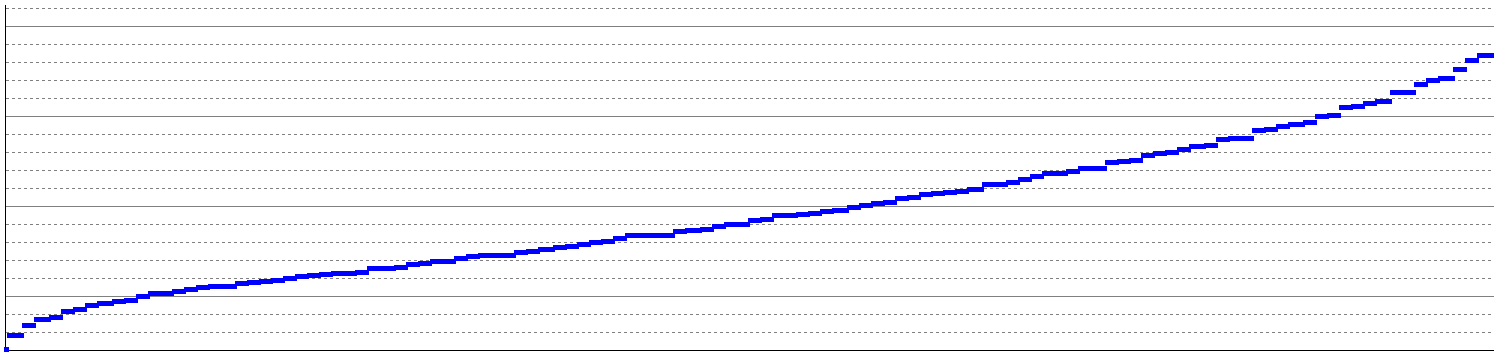
\includegraphics[width=\linewidth,height=\textheight,
keepaspectratio]{bilder/PermSize}
\caption{Anzahl der Permutationen jedes Graphenpaars}
\label{pic:PermSize}
\end{figure}

Die Tests wurden wie oben beschrieben für jeden Algorithmus ausgeführt. Das Testsystem 
war ein 2,4 GHz Doppelkernprozessor mit 4 GB RAM und Windows 7\footnote{Intel(R) Core(TM)2 
Duo T8300 @ 2,40GHz; 4,00 GB RAM; Windows 7 Service~Pack~1 (64 Bit); Windows 
Leistungsindex: Prozessor: 6,0 - RAM: 5,9; Laufzeitumgebung: .NET Framework 2.0}. 

Dauerte ein Test länger als eine Stunde, so wurde er abgebrochen. Wurden zwei Tests 
hintereinander deswegen abgebrochen, so führte dies zum Abbruch der gesamten Testreihe. 
Aufgrund der steigenden Zahl der Permutationen ist nicht zu erwarten, dass spätere Tests 
erfolgreicher sind. 

\subsection{Darstellung der Ergebnisse}
Um den Platz besser zu nutzen, wurde bei der Darstellung der Testergebnisse auf eine 
Achsenbeschriftung verzichtet. Aus diesem Grund folgt eine kurze Beschreibung der 
Darstellungen. Abbildung \ref{pic:cordExplain} stellt dies zusätzlich graphisch dar. 

\begin{figure}[htb]
\centering
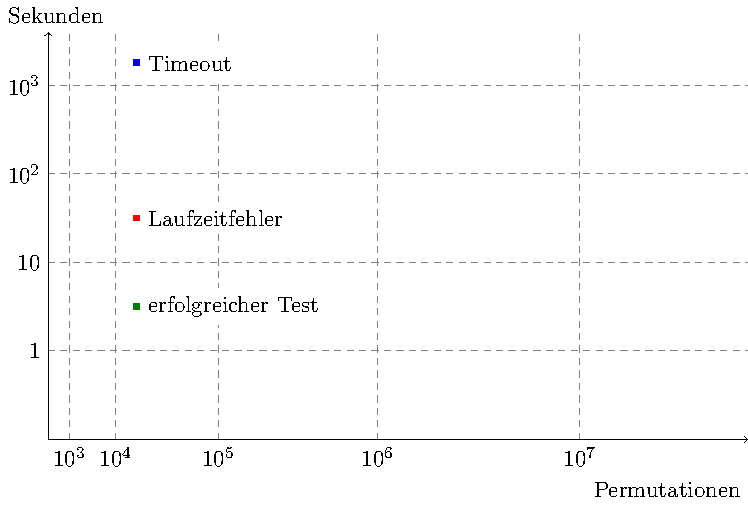
\includegraphics[width=\linewidth,height=\textheight,keepaspectratio]{bilder/empty.pdf}
%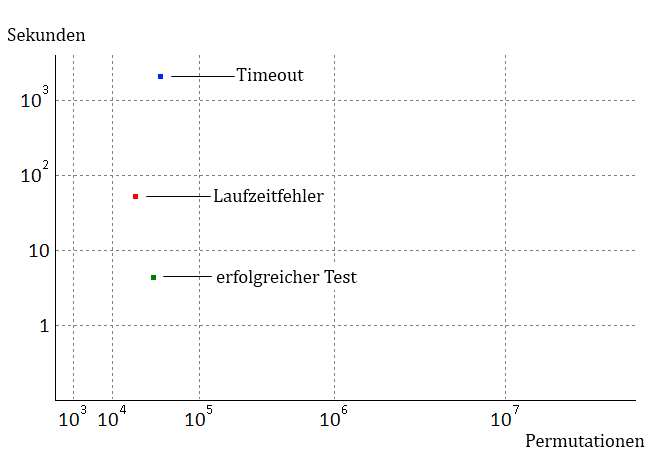
\includegraphics{bilder/empty}
\caption{Das verwendete Koordinatensystem}
\label{pic:cordExplain}
\end{figure}

\subsubsection{X-Achse}
Die Position auf der X-Achse ergibt sich aus der Position eines Tests in der 
dazugehörigen Testreihe. Da die Tests nach Anzahl ihrer Permutationen sortiert 
wurden (dargestellt in Abbildung \ref{pic:PermSize}), gibt die X-Achse diese auch 
indirekt an. Die senkrechten Hilfslinien verdeutlichen dies. Eine Hilfslinie wurde 
immer dann eingefügt, wenn die Anzahl der Permutationen eine ganzzahlige Zehnerpotenz 
überschritten hat. 

\subsubsection{Y-Achse}
Die Y-Achse stellt die Zeit in Sekunden dar, die ein Test benötigt hat. Die Einteilung 
ist logarithmisch. Begonnen wird bei $0{,}1$ Sekunden. Liegt die gemessene Laufzeit niedriger oder 
wurden gar $0{,}0$ Sekunden gemessen, so wird die Laufzeit als $0{,}1$ Sekunden behandelt. 

Die waagerechten Hilfslinien stellen die jeweils nächste Zehnerpotenz dar. So ist die 
erste Hilfslinie über der X-Achse bei $1$~Sekunde, die Zweite bei $10$~Sekunden, usw. 

\subsubsection{Farbgebung}
Jeder durchgeführte Test wird durch einen Punkt im Koordinatensystem dargestellt. Tests 
können jedoch zu unterschiedlichen Ergebnissen führen. Die Farben der Punkte stellen dies 
dar. Ist ein Test erfolgreich, wird er in \emph{grün} dargestellt. Ein \emph{blauer} 
Punkt bedeutet, dass der Test abgebrochen wurde, weil er die maximale Laufzeit 
überschritten hat. Ist der Punkt \emph{rot}, dann ist beim Test ein Fehler aufgetreten. 


\section{Testergebnisse}

\subsection{McGregor und MIS basierter Algorithmus}

\begin{figure}[htb]
\centering
\hspace*{\fill} %
\subfloat[McGregor-Alg. \label{pic:McGregor}]{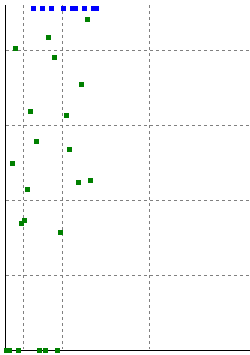
\includegraphics[width=0.25\linewidth,
keepaspectratio]{bilder/McGregor_part}}
\hspace*{\fill} %
\subfloat[MIS basierter Alg. \label{pic:MaxIndSet}]{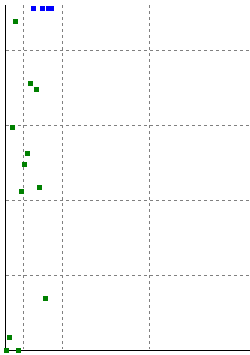
\includegraphics[width=0.25\linewidth,
keepaspectratio]{bilder/MaxIndSet_part}}
\hspace*{\fill} %
\caption{Test des McGregor- und des MIS basierten Algorithmus}
\label{pic:MG_MIS}
\end{figure}

Für beide hier dargestellten Algorithmen zeigt sich, dass sie selbst bei kleinen 
Graphen eine hohe Laufzeit haben. Die Testreihe wurde somit auch schon sehr früh 
abgebrochen. 

Die Streuung lässt sich durch zwei Eigenheiten erklären. 
Zum einen sind beide 
Algorithmen in einigen Fällen in der Lage eine optimale Lösung zu erkennen. Dann wird 
die Suche vorzeitig abgebrochen. 

Zum anderen 
arbeiten beide Algorithmen mit Kantengraphen. Dadurch, dass Kanten als Knoten behandelt 
werden und ein induzierter Teilgraph gesucht wird, ist die Anzahl der zu testenden 
Abbildungen eine andere als bei der Suche nach ECGMs auf "`normalen"' Graphen. Somit 
ist es möglich, dass Graphenpaare mit mehr Abbildungen vor Paaren mit weniger 
getestet werden.

\subsection{Probieren aller Permutationen}
\begin{figure}[htb]
\centering
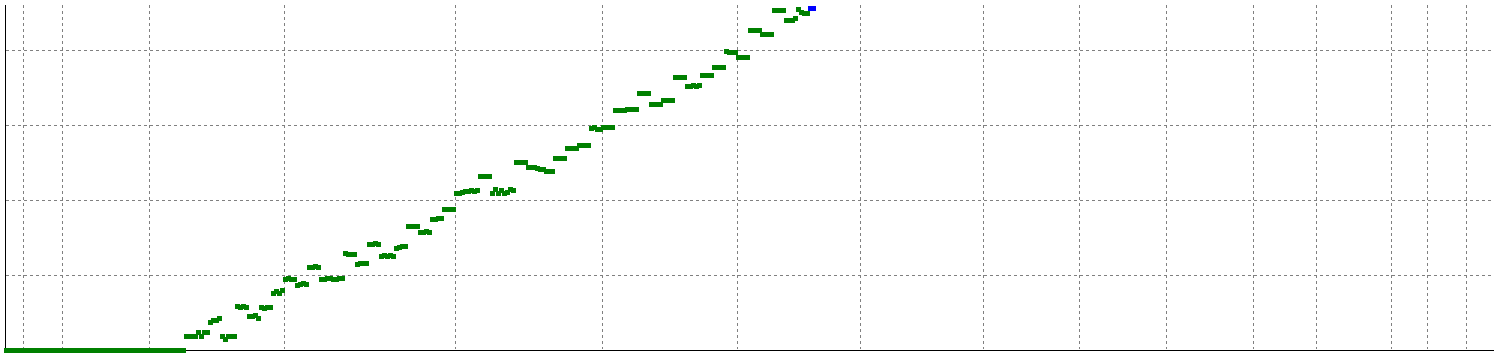
\includegraphics[width=\linewidth,height=\textheight,
keepaspectratio]{bilder/Permut}
\caption{Probieren aller möglichen ECGMs}
\label{pic:Permut}
\end{figure}

Der Zeitaufwand für das Durchprobieren aller Permutationen ist direkt von deren Anzahl 
abhängig. Da beide Achsen (annähernd\footnote{Die X-Achse ist nur nährungsweise logarithmisch 
eingeteilt. Dies liegt daran, dass die Anzahl der Permutationen der Graphenpaare nicht 
gleichmäßig steigt. Bei gleichmäßigem Anstieg würde Abbildung \ref{pic:PermSize} eine Gerade 
darstellen. Die Krümmung ist jedoch nur gering, weshalb die Steigerung nährungsweise als 
gleichmäßig angesehen werden kann.}) logarithmisch unterteilt sind, bilden die 
Laufzeiten der Tests annährend eine Gerade.

Die leichte Streuung liegt vermutlich an 
der iterativen Berechnung der nächsten Permutation anhand der aktuellen. Sind zwei 
Graphen unterschiedlich groß, so gibt es Permutationen, die das gleiche ECGM darstellen. 
Somit muss beim Erzeugen der nächsten Permutation darauf geachtet werden, dass die 
nächste Permutation auch ein neues ECGM ergibt. Dies erfordert etwas zusätzliche Rechenleistung. 
Ein rekursives Verfahren, welches die ECGMs mittels Backtracking ermittelt und nicht als 
Permutation betrachtet, könnte dazu führen, dass die Streuung geringer ist. 

Bis zu einer Größe von etwa $1{,}8 \cdot 10^6$ Permutationen ($n=10$; $m=8$) liegt die 
Laufzeit bei rund einer Sekunde. Fünf Sekunden werden mit $6{,}7 \cdot 10^6$ Permutationen 
($n=11$; $m=8$) nicht überschritten. Bei Graphenpaaren dieser Größe ist es also durchaus 
möglich, dieses Verfahren einzusetzen ohne die Geduld des Nutzers zu sehr zu belasten. 

\subsection{Branch-and-Bound (und A*)}\label{BBTest}
Das B\&B-Verfahren konnte die Testreihe vollständig durchlaufen. Kein Test musste 
abgebrochen werden, weil er über eine Stunde dauerte. Jedoch wurden viele Tests 
abgebrochen, weil die Laufzeitumgebung einen Fehler meldete (rote Punkte). Die Ursache 
dafür war das Verbrauchen von zu viel Speicher. 

\begin{figure}[htb]
\centering
\noindent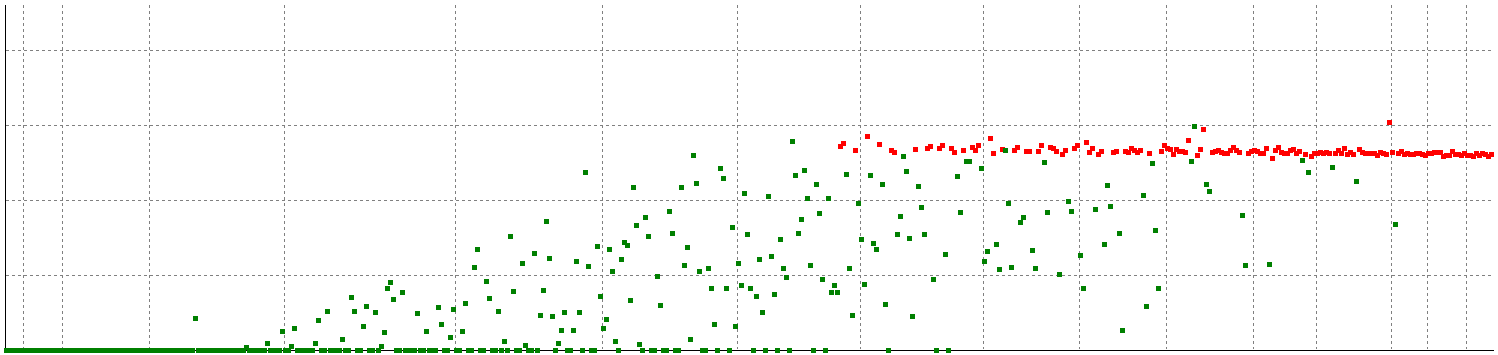
\includegraphics[width=\linewidth,height=\textheight,
keepaspectratio]{bilder/B&B}
\caption{Test des Branch-and-Bound-Verfahrens}
\label{pic:B&B}
\end{figure}

Auf den ersten Blick fällt die starke Streuung der Ergebnisse auf. Das Verfahren kann 
sehr schnell zu einem Ergebnis führen. So wurde für ein Graphenpaar mit etwa $1{,}8 \cdot 
10^{14}$ Permutationen ($n=17$; $m=15$) in $1{,}4$~Sekunden verglichen. Das erste Graphenpaar 
mit mehr als fünf Sekunden Laufzeit besitzt hingegen nur etwa $3{,}9\cdot 10^7$ 
Permutationen ($n=11$; $m=10$). Es benötigte $8{,}0$ Sekunden. 

Ebenfalls auffällig ist, dass es keine Gruppenbildung gibt. Zu jeder Anzahl an Knoten 
$n$ gibt es zwei Graphen mit unterschiedlicher Anzahl an Kanten ($d=3$ und $d=4$). 
Bei der Berechnung 
der möglichen Permutationen wird nur die Anzahl der Knoten herangezogen. Somit bilden 
sich in einer Testreihe Gruppen von jeweils zwei bzw. vier Graphenpaaren, welche die gleiche  
Anzahl an Permutationen besitzen (gut zu sehen in Abbbildung~\ref{pic:Permut}). Innerhalb 
einer solchen Gruppe unterscheiden sich die Paare nur durch die Anzahl der Kanten.
Da die Anzahl der Kanten allerdings bei der Berechnung der Schranke des B\&B-Verfahrens 
eine Rolle  spielt, liegt es somit nahe, dass die Anzahl der Kanten einen Einfluss auf 
die Rechenzeit hat.

Abbildung~\ref{pic:BBcomp} stellt erneut die Laufzeit des B\&B-Verfahrens in einem 
Ausschnitt\footnote{Die X-Achse geht von $10^6$ bis $10^{14}$ Permutationen, die 
Y-Achse von $0{,}1$ bis $100$ Sekunden.} dar. Die Färbung ist aber eine andere. Tests, 
bei denen der kleinere Graph eine geringe Kantendichte hat ($d=3$, siehe 
Abschnitt~\ref{GraphEigenschaften}) sind \emph{blau} dargestellt. Tests mit einer größeren 
Kantendichte ($d=4$) sind \emph{rot}. Wegen zu hohem Speicherverbrauch abgebrochene 
Tests wurden nicht eingezeichnet.

\begin{figure}[htb]
\centering
\noindent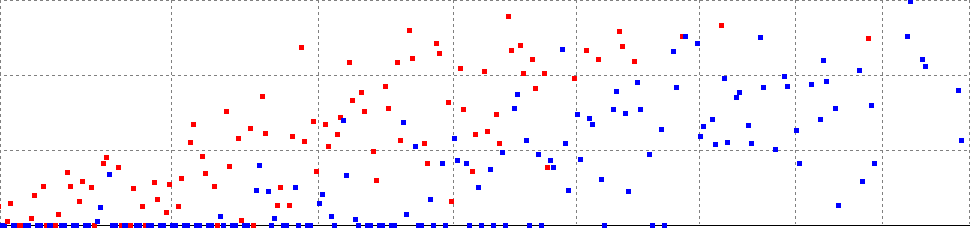
\includegraphics[width=\linewidth,height=\textheight,
keepaspectratio]{bilder/BBcomp}
\caption{B\&B-Laufzeit abhängig von der Kantendichte des kleineren Graphen}
\label{pic:BBcomp}
\end{figure}

Es ist deutlich zu sehen, dass blau markierte Tests in der Regel schneller sind als 
die roten. Beide Bereiche überlappen sich jedoch. Auch die Streuung ist bei beiden 
Varianten vorhanden. 

Dass die Kanten einen Einfluss auf die Schranke und somit auf die Laufzeit haben, 
führt zu einer weiteren Vermutung. Eventuell lässt sich die Laufzeit verringern, indem 
der Suchbaum die Knoten in Abhängigkeit ihrer anliegenden Kanten (also der Zahl ihrer 
Nachbarn) zuweist. Um dies zu überprüfen, wurde der Algorithmus leicht geändert. Vor 
der eigentlichen Suche werden die Knoten nach der Anzahl ihrer Nachbarn sortiert. Es gab zwei 
Testreihen. Eine begann den Suchbaum mit Knoten, die möglichst wenig Nachbarn hatten. 
Die Andere mit möglichst vielen. Dabei brachte die Testreihe, die Knoten mit vielen 
Nachbarn zuerst zuwies, den gewünschten Effekt. Abbildung \ref{pic:BB_Nh} stellt das 
Ergebnis dar. Das vorrangige Zuweisen der Knoten mit wenig Nachbarn führte hingegen 
zu einer Erhöhung der Laufzeit. 

\begin{figure}[htb]
\centering
\noindent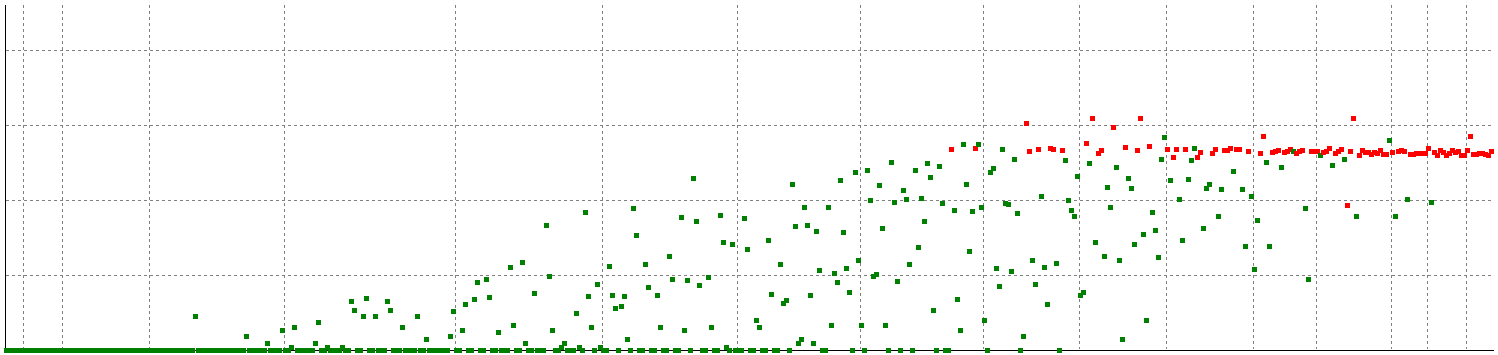
\includegraphics[width=\linewidth,height=\textheight,
keepaspectratio]{bilder/BB_Nh}
\caption{B\&B-Laufzeit, wenn Knoten mit vielen Nachbarn zuerst zugewiesen werden}
\label{pic:BB_Nh}
\end{figure}

Da die Streuung weiterhin vorhanden ist, lässt sich aus Abbildung \ref{pic:BB_Nh} nur 
schlecht sagen, ob die Verbesserung mehrheitlich ist oder nur bestimmte Graphenpaare 
betrifft. Abbildung \ref{pic:BBdif} stellt deswegen die Differenz der Laufzeiten dar. 
\emph{Rote} Punkte entsprechen dabei einer Verschlechterung der Laufzeit. Dies kann auch 
bedeuten, dass ein Test abgebrochen wurde, der vorher erfolgreich war. Hat sich die 
Laufzeit verbessert bzw. war ein Test erfolgreich, der zuvor abgebrochen werden musste, 
so wird der Punkt \emph{grün} dargestellt. 
Musste für ein Graphenpaar in beiden Testreihen der Test abgebrochen werden oder liegt 
die Zeitdifferenz unter $0{,}1$ Sekunden, ist der Test nicht eingetragen. 

\begin{figure}[htb]
\centering
\noindent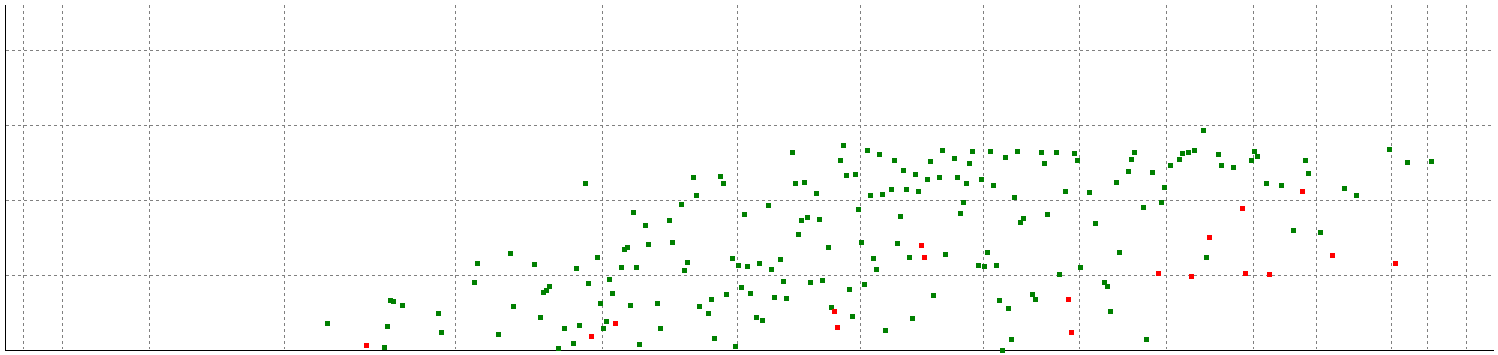
\includegraphics[width=\linewidth,height=\textheight,
keepaspectratio]{bilder/BBdif}
\caption{Laufzeitdifferenz der B\&B-Testreihen}
\label{pic:BBdif}
\end{figure}

Man kann klar erkennen, dass die überwiegende Mehrheit der Tests besser verlief. Es 
gibt aber auch Tests, die schlechter abschnitten. Es kann also nicht von einer 
generellen Verbesserung gesprochen werden. 

Das Fazit für das B\&B-Verfahren fällt weitgehend gut aus. Es ist ein exaktes Verfahren, 
welches für Graphenpaare mit niedriger und mittlerer Zahl an Permutationen in der 
Regel schnell zu einem Ergebnis führt. Das Vorsortieren der Knoten nach der Anzahl 
ihrer Nachbarn erhöht dabei die Wahrscheinlichkeit für eine kurze Laufzeit. Nachteilig 
an B\&B ist, dass es eine sehr starke Streuung besitzt. Es ist somit nur schwer 
vorhersagbar, wie lange die Berechnung für ein konkretes Graphenpaar dauert. 

\subsection{Evolutionärer Algorithmus}

Beim Testen des evolutionären Algorithmus wurde eine Population vom $1.000$ Individuen 
verwendet. Bei Mutation und Rekombination werden jeweils $1.000$ weitere Individuen 
erzeugt. Die Selektion wählt aus den nun $3.000$ Individuen die $1.000$ Besten aus. Die 
Anderen "`sterben"'. Ein Individuum wird als Optimum betrachtet, wenn nach 20 
Generationen kein besseres gefunden wurde. 

\subsubsection{Laufzeit}

\begin{figure}[htb]
\centering
\noindent\includegraphics[width=\linewidth,height=\textheight,
keepaspectratio]{bilder/evo}
\caption{Laufzeiten des evolutionären Algorithmus}
\label{pic:evo}
\end{figure}

Mittelst des evolutionären Algorithmus konnte zu jedem Paar eine 
mögliche Lösung ermittelt werden. Die Laufzeit bleibt auch bei einer hohen Anzahl 
an Permutationen verhältnismäßig gering. Das erste Graphenpaar, welches über fünf 
Sekunden benötigt, besitzt etwa $1{,}3 \cdot 10^{15}$ Permutationen ($n=15$; $m=14$). 
Die höchste Laufzeit betrug $18{,}4$ Sekunden. Das dazugehörige Graphenpaar hat etwa 
$2{,}4 \cdot 10^{18}$ mögliche Permutationen ($n=20$; $m=19$). 
 
Die sichtbare Streuung könnte zwei mögliche Ursachen haben. Zum einen ist es denkbar, 
dass die unterschiedliche Kantendichte sich auf die Zeit auswirkt. Zum anderen 
werden die Paare für eine Rekombination sowie die Änderung bei einer Mutation zufällig 
bestimmt. Ob und wann eine bessere Lösung gefunden wird, ist somit auch vom Zufall 
abhängig. 

\subsubsection{Qualität der Lösung}
Da es sich bei einem evolutionären Algorithmus nicht um ein exaktes Verfahren handelt, 
ist es nötig, die Qualität der Lösung zu betrachten. Maßgabe für die Qualität ist das  
Verhältnis der Anzahl gefundenen gemeinsamen Paare mit Kante in der exakten Lösung zur Anzahl 
in der Lösung des evolutionären Algorithmus. 

Abbildung \ref{pic:EvoQuali} stellt das Verhältnis zwischen beiden Lösungen dar. Es wurde erneut  
auf die Beschriftung verzichtet. Das Koordinatensystem unterscheidet sich jedoch von bisherigen 
Darstellungen. Die Y-Achse stellt nun das Verhältnis zwischen exakter und evolutionär ermittelter 
Lösung dar. Die Achse ist nicht mehr logarithmisch. Im Koordinatenursprung sind es $0\%$. 
Waagerechte Hilfslinien sind jeweils in $10\%$-Schritten eingezeichnet. Die X-Achse sowie die 
senkrechten Hilfslinien wurden nicht verändert. Die Farbgebung gibt zusätzlich Auskunft über die 
Zahl der gemeinsamen Paare ohne Kante. Stimmt sowohl die Zahl der Paare mit Kante als auch die 
Zahl der Paare ohne Kante mit der exakten Lösung überein, ist der Test \emph{grün} dargestellt. 
Andere Tests sind \emph{blau}. 

Da nicht für alle Graphenpaare eine exakte Lösung vorliegt, ist es auch nicht möglich zu 
jeder Lösung des evolutionären Algorithmus eine Qualität anzugeben. Die entsprechenden 
Graphenpaare sind somit nicht in Abbildung \ref{pic:EvoQuali} eingetragen. 

\begin{figure}[htb]
\centering
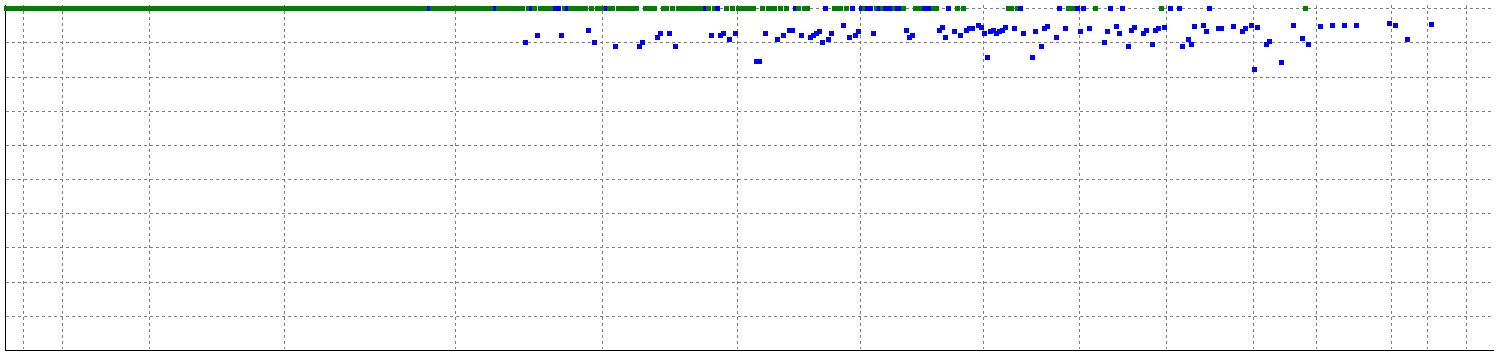
\includegraphics[width=\linewidth,height=\textheight,
keepaspectratio]{bilder/evoQuali}
\caption{Qualität der Lösungen des evolutionären Algorithmus}
\label{pic:EvoQuali}
\end{figure}

Der Evolutionäre Algorithmus liefert durchgehend gute Lösungen. Die erste Lösung unter 
$100\%$ tritt bei einem Graphenpaar mit etwa $2{,}8 \cdot 10^7$ Permutationen ($n=20$; $m=6$) 
auf. Bis etwa $10^{11}$ Permutationen haben jedoch ein Großteil der Lösungen eine 
Qualität von $100\%$. Die Mehrheit der Lösungen, die nicht vollständig übereinstimmen, 
haben eine Qualität über $90\%$. Auch schlechtere Lösungen unterschreiten die $80\%$ 
nicht. Da nicht zu jedem Paar eine Lösung bekannt ist, lässt sich jedoch nicht sagen, 
ob generell die Qualität der Lösungen so gut ist. Es ist denkbar, dass die selben 
Eigenschaften, die dazu führen, dass B\&B keine Lösung liefert, auch eine Lösung 
mit schlechter Qualität beim evolutionärem Algorithmus zur Folge haben.

\subsection{Bipartites Matching}
Die Ermittlung einer Lösung mittels bipartitem Matching ist im Vergleich zu den anderen 
getesteten Verfahren sehr schnell. Zu allen Graphenpaaren wurde in unter $0{,}1$ Sekunden 
eine Lösung ermittelt. Auf eine Darstellung der Laufzeit wird deshalb verzichtet. 

Interessant ist die Qualität der Lösungen, denn es handelt sich um eine Heuristik. Es 
wurde jedoch nicht das Gewicht des Matchings genommen, da es nur eine Schätzung ist und nicht 
die realen Kosten angibt. Stattdessen werden die gemeinsamen Paare genommen, 
die sich durch das Matching ergeben. Abbildung \ref{pic:BipQuali} stellt die Qualität 
des Verfahrens dar. Die Darstellung ist analog zur Qualitätsdarstellung des evolutionären 
Algorithmus. 

\begin{figure}[htb]
\centering
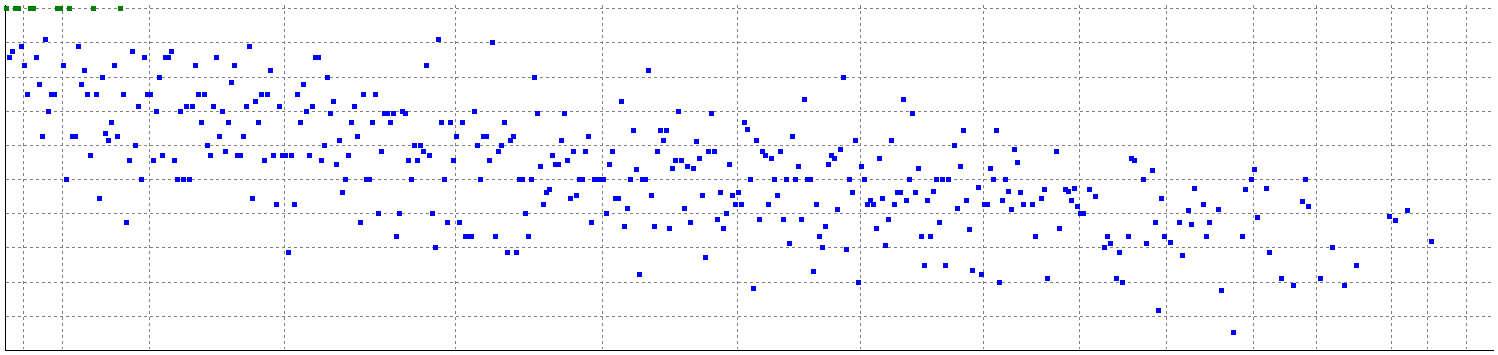
\includegraphics[width=\linewidth,height=\textheight,
keepaspectratio]{bilder/bipQuali}
\caption{Qualität der Lösungen des bipartiten Matchings}
\label{pic:BipQuali}
\end{figure}

Neben der starken Streuung der Ergebnisse sieht man auch, dass die Qualität bei größeren 
Graphenpaaren deutlich abnimmt. Eine mögliche Erklärung für die Abnahme ist, dass die 
Zahl der Kanten in den Graphen linear mit deren Größe steigt. Die Anzahl der Knotenpaare 
steigt jedoch quadratisch. Die Wahrscheinlichkeit, dass bei zwei Knotenpaaren auch beide 
eine Kante besitzen, nimmt somit ab.

Abbildung \ref{pic:RndQuali} stellt die Qualität einer weiteren Testreihe dar. Hierbei 
wurden bei jedem Test zehn zufällige Permutationen erstellt und die Beste dann als Lösung 
ausgegeben. Es ist zu sehen, dass die Qualität der mittels bipartitem Matching ermittelten 
Lösung sich kaum von der Qualität der zufällig erzeugten Lösungen unterscheidet. 

\begin{figure}[htb]
\centering
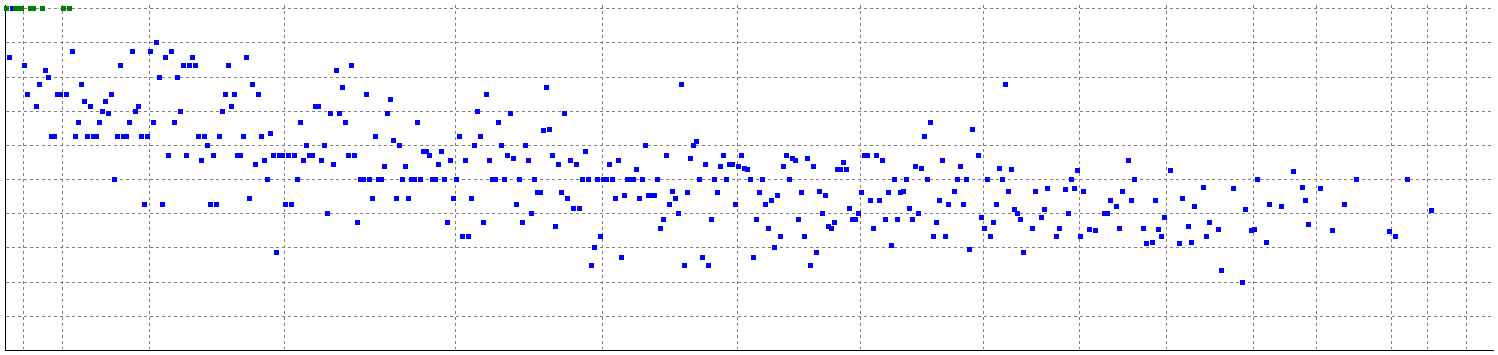
\includegraphics[width=\linewidth,height=\textheight,
keepaspectratio]{bilder/rndQuali}
\caption{Qualität von zufälligen Lösungen}
\label{pic:RndQuali}
\end{figure}

Das Fazit für das bipartite Matching fällt negativ aus. Zwar ist es ein sehr schnelles 
Verfahren, jedoch führt die Heuristik nicht zu Lösungen mit hoher Qualität. Die Qualität 
ist auch nicht besser als zufällig ermittelte Lösungen. 


\chapter{Praktische Umsetzung}\label{chp:Umsetzung}
Dieses Kapitel stellt am Beispiel der Lotka-""Volterra-""Form~(LV-Form) ein Konzept 
für die praktische Umsetzung dar.

\section{Lotka-Volterra-Form}
Die Lotka-Volterra-Regeln (LV-Regeln) sind ein Regelwerk "`zur quantitativen Beschreibung 
der Populationsdynamik in Räuber-""Beute-""Beziehungen"' \cite{wikiD:LVR}. Sie wurden 
1925 und 1926 von Alfred Lotka und Vito Volterra formuliert. Die LV-Form ist ein Modell, 
welches auf den LV-Regeln basiert. 

\subsection{Elemente}
Eine LV-Form besteht aus drei Elementen: \emph{Populationen}, \emph{Ereignisse} 
und \emph{Parameter}. Abbildung \ref{pic:LVFKomponenten} stellt diese dar.

%\begin{figure}[htb]
%\centering
%\hspace*{\fill} 
%\subfloat[Population\label{pic:Population}]
%         {
\includegraphics[width=0.2\linewidth,keepaspectratio]{bilder/lvfPopulation}}
%\hspace*{\fill} 
%\subfloat[Ereignis\label{pic:Ereignis}]
%         {\includegraphics[width=0.2\linewidth,keepaspectratio]{bilder/lvfEreignis}}
%\hspace*{\fill} 
%\subfloat[Parameter\label{pic:Parameter}]
%         {\includegraphics[width=0.2\linewidth,keepaspectratio]{bilder/lvfParameter}}
%\hspace*{\fill} 
%\caption{Elemente der LV-Form}
%\label{pic:LVFKomponenten}
%\end{figure}

\begin{figure}[htb]
\centering
\hspace*{\fill} 
\subfloat[Population\label{pic:Population}]
         {\begin{tikzpicture}
  [thick,
   lvgNode/.style={draw,minimum width=2cm, minimum height=1cm},
   popN/.style={cloud,cloud puffs=9,lvgNode, minimum height=1.5cm},
   parN/.style={ellipse,lvgNode},
   eveN/.style={rectangle,rounded corners=0.25cm,lvgNode},
  ]

 \node[popN] at (0,0) {};
\end{tikzpicture}}
\hspace*{\fill} 
\hspace*{\fill} 
\subfloat[Ereignis\label{pic:Ereignis}]
         {\begin{tikzpicture}
  [thick,
   lvgNode/.style={draw,minimum width=2cm, minimum height=1cm},
   popN/.style={cloud,cloud puffs=9,lvgNode, minimum height=1.5cm},
   parN/.style={ellipse,lvgNode},
   eveN/.style={rectangle,rounded corners=0.25cm,lvgNode},
  ]

 \node[eveN] at (0,0) {};
\end{tikzpicture}}
\hspace*{\fill} 
\hspace*{\fill} 
\subfloat[Parameter\label{pic:Parameter}]
         {\begin{tikzpicture}
  [thick,
   lvgNode/.style={draw,minimum width=2cm, minimum height=1cm},
   popN/.style={cloud,cloud puffs=9,lvgNode, minimum height=1.5cm},
   parN/.style={ellipse,lvgNode},
   eveN/.style={rectangle,rounded corners=0.25cm,lvgNode},
  ]

 \node[parN] at (0,0) {};
\end{tikzpicture}}
\hspace*{\fill} 
\caption{Elemente der LV-Form}
\label{pic:LVFKomponenten}
\end{figure}

\emph{Populationen} sind die Basiselemente. Sie stellen eine Gruppe von Lebewesen dar. 

Ein \emph{Ereignis} ist eine gerichtete Verbindung zweier Populationen miteinander. 
Es kann auch eine Population mit sich selbst verbunden werden. Ereignisse stellen 
Handlungen oder Geschehen in einer Population dar, die Auswirkungen auf die 
Ziel-Population haben.

\emph{Parameter} beeinflussen Ereignisse. Sie sind somit auch immer auf (mindestens) ein 
Ereignis gerichtet. Sie können zusätzlich von Populationen abhängig sein. 

%\begin{figure}[htb]
%\centering
%\includegraphics[width=\linewidth,height=\textheight,
%keepaspectratio]{bilder/LVFConns}
%\caption{Mögliche Verbindungen in einer LV-Form}
%\label{pic:LVFConns}
%\end{figure}

\begin{figure}[htb]
\centering
\begin{tikzpicture}
  [thick,node distance=1.5cm,
   lvgNode/.style={draw,minimum width=2cm, minimum height=1cm},
   popN/.style={cloud,cloud puffs=9,lvgNode,shape aspect=1.5,inner sep=-5pt, minimum height=1.5cm},
   parN/.style={ellipse,lvgNode,shape aspect=2},
   eveN/.style={rectangle,rounded corners=0.25cm,shape aspect=2,lvgNode},
  ]

 \node[popN] (pop1)                       {Popul. 1};
 \node[parN] (par)  [above right=of pop1] {Parameter};
 \node[eveN] (eve)  [below right=of par]  {Ereignis};
 \node[popN] (pop2) [right=of eve]        {Popul. 2};

 \draw [->,out=90,in=180] (pop1) to (par);
 \draw [->,out=0,in=90]   (par)  to (eve);
 \draw [->]               (pop1) to (eve);
 \draw [->]               (eve)  to (pop2);
\end{tikzpicture}
\caption{Mögliche Verbindungen in einer LV-Form}
\label{pic:LVFConns}
\end{figure}

\subsection{Formale Umsetzung}
Mit den oben beschriebenen Regeln lässt sich eine LV-Form aus 
Populationen, Ereignissen und Paramtern formal beschreiben.

\begin{mydef}[Lotka-Volterra-Form]\label{def:LVF}
Eine Lotka-Volterra-Form $\Lambda$ ist ein 3-Tupel $\Lambda=(\Pi, \Sigma, 
\Phi)$. Dabei sind:
\begin{itemize}
	\item $\Pi$ eine endliche Menge von Populationen,
	\item $\Sigma \subseteq \Pi \times \Pi$ die Menge an Ereignissen und
	\item $\Phi \subseteq \wp(\Pi) \times (\wp(\Sigma) \backslash \{\emptyset\})$
	      die Menge an Parametern\footnote{$\wp(M)=\{T\ |\ T\subseteq M\}$ ist
	      die Potenzmenge (die Menge aller Teilmengen) von M.}.
\end{itemize}
\end{mydef}

\subsection{Umsetzung als Graph}
Die nun formal beschriebene LV-Form lässt sich auch als Graph umsetzen. Dabei 
sind Populationen, Ereignisse und Parameter jeweils Knoten. Die Kanten ergeben 
sich direkt aus den in Definition \ref{def:LVF} beschrieben Bedingungen. Der 
so entstehende gerichtete Graph sei dann ein Lotka-Volterra-Graph (LVG).

\begin{mydef}[Lotka-Volterra-Graph]
Gegeben sei eine LV-Form $\Lambda=(\Pi, \Sigma, \Phi)$. Der dazugehörige 
gerichtete Lotka-Volterra-Graph $G=(V,E)$ sei wie folgt definiert:

Die Knotenmenge $V$ ist die Vereinigungsmenge der Populationen, Ereignisse 
und Parameter.
\[ V=\Pi \cup \Sigma \cup \Phi \]

Die Kantenmenge $E$ ist die Vereinigung aus der durch Ereignisse erzeugten 
Kantenmenge $E_\Sigma$ sowie der durch Parameter erzeugten Kantenmenge $E_{\Pi\Phi}$ 
und $E_{\Phi\Pi}$. Dabei stellt $E_{\Pi\Phi}$ die Kanten von Populationen zu 
Parametern und $E_{\Phi\Sigma}$ von Parametern zu Ereignissen dar. 
\[ E=E_\Sigma \cup E_{\Pi\Phi} \cup E_{\Phi\Sigma} \]

Für jedes Ereignis $e=(p,q)\in\Sigma$ ist jeweils eine Kante zwischen dem Ereignis 
und den beiden Populationen $p$ und $q$ in $E_\Sigma$ enthalten. 
\[ E_\Sigma=\{(p,e),(e,q)\ |\ e \in \Sigma\} \]

In $E_{\Pi\Phi}$ befindet sich für jeden Parameter $\varphi=(P_\Pi,P_\Sigma) \in \Phi$ 
jeweils eine Kante zwischen den Populationen $\pi \in P_\Pi$ und dem Parameter $\varphi$.
\[ E_{\Pi\Phi}=\bigcup_{\varphi \in \Phi}\{(\pi,\varphi)\ |\ \pi \in P_\Pi\} \]

Des weiteren ist in $E_{\Phi\Sigma}$ für jeden Parameter $\varphi=(P_\Pi,P_\Sigma) \in \Phi$
jeweils eine Kante vom Parameter $\varphi$ zu jedem Ereignis $e \in P_\Sigma$ vorhanden.
\[ E_{\Phi\Sigma}=\bigcup_{\varphi \in \Phi}\{(\varphi,e)\ |\ e \in P_\Sigma\} \]
\end{mydef}

Der so erzeugte LVG lässt sich nun mit anderen Graphen vergleichen.

\section{Veringerung der Komplexität}
Angenommen, eine LV-Form besitzt vier Populationen, pro Population zwei Ereignisse 
und fünf Parameter. Der dazugehörige LVG hat dann 17~Knoten. Vergleicht 
man den LVG mit einem dazu isomorphen Graphen, so gibt es etwa $3{,}6 \cdot 10^{14}$ 
ECGMs. Das B\&B-Verfahren hat in dieser Größenordnung eine hohe Wahrscheinlichkeit 
nicht erfolgreich zu sein. Bei den entsprechenden Tests (Abschnitt \ref{BBTest}) 
mussten die meisten von ihnen abgebrochen werden, weil der Speicherverbrauch zu hoch war. 

\subsection{Vorgabe von Knoten}\label{sec:VorgabeKnoten}
Eine Möglichkeit, die Anzahl der ECGMs zu senken, ist es, dem Lerner Knoten 
vorzugeben. So könnten beispielsweise die Population vorgegeben werden. 
Die entsprechenden Knoten sind dann fest den Populationsknoten in der 
Musterlösung zugeordnet. Die Anzahl der ECGMs sinkt dann auf etwa $6{,}2 \cdot 10^9$. 

Es besteht vermutlich auch die Chance, dass sich durch die Vorgabe schneller deutliche 
Schranken bilden, also dass schneller abgeschätzt werden kann, wie viele Kanten der gemeinsame 
Teilgraph höchstens haben wird. Die Vermutung basiert darauf, dass die zugewiesenen Knoten auch 
Auswirkungen auf die Kanten und somit auf die benachbarten Knoten haben. Gibt es ohne 
Vorgabe beispielsweise für ein verbundenes Paar aus einer Population und einem Ereignis 
vier oder mehr mögliche Abbildungen, so gibt es mit Vorgabe nur noch ein oder zwei. 
Dies liegt daran, dass die Population eindeutig bestimmt werden kann. Somit bleiben 
als mögliche Zuordnungen für das Ereignis nur die Ereignisse der Musterlösung, die 
mit der Population verbunden sind.

\subsection{Knotenfärbung}
Eine weitere Möglichkeit besteht darin, die Knoten eines Graphen in Gruppen zu 
unterteilen, sie zu färben.

\begin{mydef}[Knotenfärbung]
Gegeben sei ein Graph $G=(V,E)$. Eine Knotenfärbung $f$ ist eine Abbildung 
$f: V \rightarrow \mathbb{N}$. Die Farbe eines Knotens $v$ ist dann $f(v)$.
\end{mydef}

Nun erlaubt man in einem ECGM nur Zuweisungen, wenn beide Knoten die gleiche Farbe 
besitzen. Für einen LVG bietet es sich an, die Knoten in drei Farben zu unterteilen: 
je eine Farbe für Populationen, Ereignisse und Parameter. Auch die Vorgabe von Knoten 
lässt sich mittels Färbung umsetzen. Jeder vorgegebene Knoten bekommt eine eigene Farbe. 

Mittels Färbung lässt sich nun die Zahl der möglichen ECGMs von $G_1=(V_1,E_1)$ nach 
$G_2=(V_2,E_2)$ stark reduzieren. Es seien $n_i$ und $m_i$ die Anzahl der Knoten in $G_1$ 
bzw. $G_2$, welche die Farbe $i$ haben.
\begin{align*}
n_i&=\big| \{v\ |\ v \in V_1 \wedge f(v)=i\}\big| \\
m_i&=\big| \{v\ |\ v \in V_2 \wedge f(v)=i\}\big| 
\end{align*}

Es sei dann $p_i$ die Anzahl der ECGMs innerhalb einer Farbe.
\[ p_i=\left\{\begin{array}{ll}
                \frac{n_i!}{(n_i-m_i)!} & n_i \geq m_i \\
                \frac{m_i!}{(m_i-n_i)!} & \text{sonst}
              \end{array}\right. \]
              
Die Gesamtzahl $p$ der ECGMs ist nun das Produkt aller $p_i$.
\[ p=\prod_{i \in \mathbb{N}}p_i \]

Das Beispiel von oben hat dann, wenn es mit einem isomorphen Graphen verglichen wird, 
$4{,}8 \cdot 10^6$ mögliche ECGMs. In der Testreihe des B\&B-Verfahrens, in der die Knoten 
nach Zahl ihrer Nachbarn sortiert wurden (siehe Abbildung \ref{pic:BB_Nh}), wurden alle Tests 
in der Größenordnung von $10^6$ bis $10^7$ Permutationen erfolgreich in unter $1$~Sekunde 
beendet.

\section{Auswertung eines ECGMs}
Nach Ermittlung eines ECGMs ist der nächste Schritt die Auswertung. In der hier vorgestellten 
Variante wird ein Fehlergraph gebildet. Anschließend erfolgt eine Mustersuche auf Basis von
TGI.

\subsection{Fehlergraph}
Die Idee an einem Fehlergraph ist es, dass man beide Graphen zusammenfügt. Zusätzlich 
markiert man die Knoten und Kanten abhängig davon, ob sie hinzugefügt, entfernt oder übernommen 
wurden. Auf diese Weise lässt sich in diesem neuen Graphen nach Mustern suchen. Der so erzeugte Graph 
sei ein Fehlergraph.

\begin{mydef}[Fehlergraph]
Gegeben seien zwei Graphen $G_1=(V_1,E_2)$ und $G_2=(V_2,E_2)$ sowie ein ECGM 
$\varphi:\hat{V}_1 \rightarrow \hat{V}_2$ mit $\hat{V}_1 \subseteq V_1$ und 
$\hat{V}_2 \subseteq V_2$. Aus $G_1$, $G_2$ und $\varphi$ ergeben sich zusätzlich 
$V_d$, $V_a$ $E_d$ und $E_a$ (siehe Abschnitt \ref{sec:Graphabstand}).

Ein Fehlergraph von $G_1$, $G_2$ und $\varphi$ ist dann ein 3-Tupel $F=(V_F,E_F,\alpha)$. 
Dabei sind:
\begin{itemize}
	\item $V_F=V_1 \cup V_a$ die Menge der Knoten,
	\item $E_F=E_1 \cup E_a$ die Menge der Kanten und
	\item $\alpha: V \cup E \rightarrow \{r,g,b\}$ die Markierung der Knoten und Kanten.
\end{itemize}

Dabei wird ein Element des Graphen (ein Knoten oder eine Kante) mit $r$ markiert, 
wenn es entfernt wird. Es erhält $g$ als Markierung, wenn es hinzugefügt wird. 
Ist ein Element in beiden Graphen vorhanden (wird übernommen), dann wird es mit $b$ 
markiert.
\[
\alpha(x)=\left\{\begin{array}{ll}
                    r & x \in V_d \cup E_d \\
                    g & x \in V_a \cup E_a \\
                    b & sonst
                 \end{array}\right.
\]
\end{mydef}

Der so erzeugte Fehlergraph $F$ ist nun ein Graph, der alle Informationen aus den Graphen 
$G_1$ und $G_2$ sowie dem ECGM $\varphi$ enthält. Abbildung \ref{pic:Fehlergraph} stellt dies dar. 
Die Knoten und Kanten sind dabei entsprechend ihrer Markierung in rot, grün und blau 
dargestellt.

%\begin{figure}[htb]
%\centering
%\subfloat[ Eingabe des Lerners\label{pic:FG_Eingabe}]{\includegraphics[width=0.4\linewidth,
%keepaspectratio]{bilder/bspFGEingabe}}
%\hspace{1.2cm} 
%\subfloat[Musterlösung\label{pic:FG_Musterloesung}]{\includegraphics[width=0.4\linewidth,
%keepaspectratio]{bilder/bspFGLsg}}
%\hspace{1.2cm} 
%\subfloat[erzeugter Feh"-ler"-graph\label{pic:FG}]{\includegraphics[width=0.4\linewidth,
%keepaspectratio]{bilder/bspFGAusgabe}}
%\caption{Beispiel für einen Fehlergraph}
%\label{pic:Fehlergraph}
%\end{figure}

\begin{figure}[htb]
\centering
\hspace*{\fill} 
\subfloat[Eingabe des Lerners\label{pic:FG_Eingabe}]
{\begin{tikzpicture}
  [normalN/.style={circle,draw,minimum size=0.8cm},
   thick]

  \node[normalN] (c) at   (0:0)   {4};
  \node[normalN] (t) at  (90:1.6) {1};
  \node[normalN] (l) at (210:1.6) {2};
  \node[normalN] (r) at (-30:1.6) {3};
  
  \path (210:1.6)+(120:1.6) node[normalN,black!0] (ll) {};
  \path (-30:1.6)+ (60:1.6) node[normalN,black!0] (rr) {};

  \draw [] (c) -- (t);
  \draw [] (c) -- (l);
  \draw [] (c) -- (r);
  
  \draw [] (t) -- (l);
  \draw [] (t) -- (r);
  \draw [] (l) -- (r);
  
  %\draw [] (l) -- (ll);
  %\draw [] (r) -- (rr);
\end{tikzpicture}}
\hspace*{\fill} 
\subfloat[Musterlösung\label{pic:FG_Musterloesung}]
{\begin{tikzpicture}
  [normalN/.style={circle,draw,minimum size=0.8cm},
   thick]

  \node[normalN] (c) at   (0:0)   {c};
  \node[normalN] (t) at  (90:1.6) {a};
  \node[normalN] (l) at (210:1.6) {b};
  \node[normalN] (r) at (-30:1.6) {d};
  
  \path (210:1.6)+(120:1.6) node[normalN] (ll) {e};
  \path (-30:1.6)+ (60:1.6) node[normalN] (rr) {f};

  \draw [] (c) -- (t);
  %\draw [] (c) -- (l);
  %\draw [] (c) -- (r);
  
  \draw [] (t) -- (l);
  \draw [] (t) -- (r);
  \draw [] (l) -- (r);
  
  \draw [] (l) -- (ll);
  \draw [] (r) -- (rr);
\end{tikzpicture}}
\hspace*{\fill} \\ \hspace*{\fill} 
\subfloat[erzeugter Feh"-ler"-graph\label{pic:FG}]
{\begin{tikzpicture}
  [normalN/.style={circle,draw,minimum size=0.8cm},
   thick,draw=blue]

  \node[normalN] (c) at   (0:0)   {4c};
  \node[normalN] (t) at  (90:1.6) {1a};
  \node[normalN] (l) at (210:1.6) {2b};
  \node[normalN] (r) at (-30:1.6) {3d};
  
  \path (210:1.6)+(120:1.6) node[normalN,draw=darkgreen] (ll) {e};
  \path (-30:1.6)+ (60:1.6) node[normalN,draw=darkgreen] (rr) {f};

  \draw [] (c) -- (t);
  \draw [red] (c) -- (l);
  \draw [red] (c) -- (r);
  
  \draw [] (t) -- (l);
  \draw [] (t) -- (r);
  \draw [] (l) -- (r);
  
  \draw [darkgreen] (l) -- (ll);
  \draw [darkgreen] (r) -- (rr);
\end{tikzpicture}}
\hspace*{\fill} 
\caption{Beispiel für einen Fehlergraph}
\label{pic:Fehlergraph}
\end{figure}

\subsection{Mustererkennung}
Das Erkennen von Mustern in einem Fehlergraphen lässt sich über Teilgraphisomorphie (TGI) realisieren. 
Dabei stellt man die Muster als Graphen dar, zu denen dann isomorphe Teilgraphen im 
Fehlergraphen gesucht werden. Zwar ist TGI auch NP-vollständig, ein Muster ist aber 
höchstens so groß wie der Fehlergraph. Nimmt man zusätzlich an, dass die gesuchten Muster 
deutlich kleiner sind als die Fehlergraphen, so sollte selbst mit einfachen Algorithmen wie 
Backtracking die Laufzeit in verträglichem Maße bleiben.

\subsubsection{Elementare Muster}
Die zu suchenden Muster sind Graphen. Ihre Elemente sind Knoten und Kanten. Somit stellt 
ein Knoten bzw. eine Kante ein elementares Muster dar. Dabei ist vor allem die Markierung 
interessant. Die drei bei Fehlergraphen verwendeten Markierungen lassen sich erweitern. 
So wäre es eine Möglichkeit, Knoten und Kanten mit beliebiger Markierung zuzulassen. 
Abbildung \ref{pic:bspElementareMuster} stellt mögliche elementare Varianten für Knoten dar. Ist eine 
beliebige Markierung zulässig, so wird der Knoten gestrichelt gezeichnet. Kanten verhalten 
sich dazu analog.

Dieses Prinzip lässt sich auch auf die Färbung von Knoten erweitern. So ist es denkbar, 
dass man in dem Fehlergraphen eines LVG etwas sucht. Ein elementares Muster wäre hier, 
dass ein Ereignis entfernt wird (Abbildung~\ref{pic:bspEreignisLoeschen}).

%\begin{figure}[htb]
%\centering
%\hspace*{\fill} 
%\subfloat[belibiger Knoten\label{pic:bspBelibiegerKnoten}]
%         {\includegraphics[width=0.2\linewidth,keepaspectratio]{bilder/bspBelibiegerKnoten}}
%\hspace*{\fill} 
%\subfloat[entferntes Ereignis\label{pic:bspEreignisLoeschen}]
%         {\includegraphics[width=0.2\linewidth,keepaspectratio]{bilder/bspEreignisLoeschen}}
%\hspace*{\fill} 
%\subfloat[gemeinsame Population\label{pic:bspGemeinsamePopulation}]
%         {\includegraphics[width=0.2\linewidth,keepaspectratio]{bilder/bspGemeinsamePopulation}}
%\hspace*{\fill} 
%\caption{Beispiele für elementare Knotenmuster}
%\label{pic:bspElementareMuster}
%\end{figure}

\begin{figure}[htb]
\centering
\hspace*{\fill} 
\subfloat[beliebiger Knoten\label{pic:bspBelibiegerKnoten}]
         {\begin{tikzpicture}
  [thick,
   lvgNode/.style={draw,minimum width=2cm, minimum height=1cm},
   normalN/.style={draw,minimum size=1.25cm,circle},
   popN/.style={cloud,cloud puffs=9,lvgNode, minimum height=1.5cm},
   parN/.style={ellipse,lvgNode},
   eveN/.style={rectangle,rounded corners=0.25cm,lvgNode},
  ]

 \node[normalN,dashed] at (0,0) {};
 \node[minimum width=3cm, minimum height=1.5cm] at (0,0) {};
\end{tikzpicture}}
\hspace*{\fill} 
\hspace*{\fill} 
\subfloat[entferntes Ereignis\label{pic:bspEreignisLoeschen}]
         {\begin{tikzpicture}
  [thick,
   lvgNode/.style={draw,minimum width=2cm, minimum height=1cm},
   normalN/.style={draw,minimum size=1.25cm,circle},
   popN/.style={cloud,cloud puffs=9,lvgNode, minimum height=1.5cm},
   parN/.style={ellipse,lvgNode},
   eveN/.style={rectangle,rounded corners=0.25cm,lvgNode},
  ]

 \node[eveN,red] at (0,0) {};
 \node[minimum width=3cm, minimum height=1.5cm] at (0,0) {};
\end{tikzpicture}}
\hspace*{\fill} 
\hspace*{\fill} 
\subfloat[gemeinsame Population\label{pic:bspGemeinsamePopulation}]
         {\begin{tikzpicture}
  [thick,
   lvgNode/.style={draw,minimum width=2cm, minimum height=1cm},
   normalN/.style={draw,minimum size=1.25cm,circle},
   popN/.style={cloud,cloud puffs=9,lvgNode, minimum height=1.5cm},
   parN/.style={ellipse,lvgNode},
   eveN/.style={rectangle,rounded corners=0.25cm,lvgNode},
  ]

 \node[popN,blue] at (0,0) {};
 \node[minimum width=2.3cm, minimum height=1.5cm] at (0,0) {};
\end{tikzpicture}}
\hspace*{\fill} 
\caption{Beispiele für elementare Knotenmuster}
\label{pic:bspElementareMuster}
\end{figure}

\subsubsection{Einfache Muster}
Mittels der elementaren Muster lassen sich nun größere Muster entwerfen. So lässt 
sich mit dem Muster in Abbildung \ref{pic:bspKnotenZuViel} beispielsweise erkennen, dass der 
Lerner lediglich einen Knoten zu viel hinzugefügt hat. Betrachtet 
man nur die Zahl der entfernten und hinzugefügten Knoten, so würde man dem Lerner 
zwei überflüssige Kanten, einen überflüssigen Knoten 
und eine fehlende Kante anlasten. Das Muster ermöglicht somit eine andere Bewertung.

%\begin{figure}[htb]
%\centering
%\includegraphics[width=0.7\linewidth,height=\textheight,
%keepaspectratio]{bilder/bspKnotenZuViel}
%\caption{Knoten zu viel}
%\label{pic:bspKnotenZuViel}
%\end{figure}

\begin{figure}[htb]
\centering
\begin{tikzpicture}
  [thick,node distance=5cm,
   lvgNode/.style={draw,minimum width=2cm, minimum height=1cm},
   normalN/.style={draw,minimum size=1.25cm,circle},
   popN/.style={cloud,cloud puffs=9,lvgNode, minimum height=1.5cm},
   parN/.style={ellipse,lvgNode},
   eveN/.style={rectangle,rounded corners=0.25cm,lvgNode},
  ]

 \node[normalN,dashed] (l) {};
 \node[normalN,dashed] (r) [right=of l] {};
 
 \draw[out=45,in=135,red]       (l) .. controls +(45:2cm) and +(135:2cm) ..
                                       node [normalN,fill=white] {}         (r);

 \draw[darkgreen] (l) .. controls +(-45:2cm) and +(-135:2cm) .. (r);

\end{tikzpicture}
\caption{Knoten zu viel}
\label{pic:bspKnotenZuViel}
\end{figure}

Die Abbildungen \ref{pic:bspFalscheRichtung} und \ref{pic:bspFalschePopulation} zeigen zwei 
weitere Beispiele. Im ersten Fall wurde 
eine Kante in die falsche Richtung eingetragen. Das zweite Beispiel verwendet zusätzlich 
die Knotenfärbung. Es gibt an, dass ein Ereignis auf die falsche Population gerichtet ist.

%\begin{figure}[htb]
%\centering
%\includegraphics[width=0.7\linewidth,height=\textheight,
%keepaspectratio]{bilder/bspFalscheRichtung}
%\caption{Falsche Richtung einer Kante}
%\label{pic:bspFalscheRichtung}
%\end{figure}

\begin{figure}[htb]
\centering
\begin{tikzpicture}
  [thick,node distance=5cm,
   lvgNode/.style={draw,minimum width=2cm, minimum height=1cm},
   normalN/.style={draw,minimum size=1.25cm,circle},
   popN/.style={cloud,cloud puffs=9,lvgNode, minimum height=1.5cm},
   parN/.style={ellipse,lvgNode},
   eveN/.style={rectangle,rounded corners=0.25cm,lvgNode},
  ]

 \node[normalN,dashed] (l) {};
 \node[normalN,dashed] (r) [right=of l] {};
 
 \draw[->,out=45,in=180,red]       (l) to (r);
 \draw[<-,out=0,in=-135,darkgreen] (l) to (r);

\end{tikzpicture}
\caption{Falsche Richtung einer Kante}
\label{pic:bspFalscheRichtung}
\end{figure}

%\begin{figure}[htb]
%\centering
%\includegraphics[width=0.7\linewidth,height=\textheight,
%keepaspectratio]{bilder/bspFalschePopulation}
%\caption{Ereignis zielt auf falsche Population}
%\label{pic:bspFalschePopulation}
%\end{figure}

\begin{figure}[htb]
\centering
\begin{tikzpicture}
  [thick,node distance=3cm,
   lvgNode/.style={draw,minimum width=2cm, minimum height=1cm},
   normalN/.style={draw,minimum size=1.25cm,circle},
   popN/.style={cloud,cloud puffs=9,lvgNode, minimum height=1.5cm},
   parN/.style={ellipse,lvgNode},
   eveN/.style={rectangle,rounded corners=0.25cm,lvgNode},
  ]

 \node[popN,dashed] (pl)  at (-3.5,0)    {};
 \node[eveN,blue]   (ev)  at    (0,0)    {};
 \node[popN,dashed] (prt) at  (3.5,1.2)  {};
 \node[popN,dashed] (prb) at  (3.5,-1.2) {};
 
 \draw[->,blue]                   (pl) to (ev);
 \draw[->,out=0,in=180,darkgreen] (ev) to (prb);
 \draw[->,out=0,in=180,red]       (ev) to (prt);

\end{tikzpicture}
\caption{Ereignis zielt auf falsche Population}
\label{pic:bspFalschePopulation}
\end{figure}

\subsubsection{Musterhierarchie}
Bildet man aus einfachen Mustern größere, so entsteht dabei auch eine Hierarchie. Das 
Erkennen dieser Hierarchie kann Vorteile für die Suche nach Mustern und die Bewertung der 
Eingabe des Lerners haben.

Ist ein kleines Muster Teil eines größeren, so hat dies zur Folge, dass das größere 
nur dann vorhanden ist, wenn auch das kleinere gefunden wurde. Mit einer Hierachie 
lässt sich somit der Aufwand für die Mustersuche verringern, indem zuerst kleinere Muster 
gesucht werden. Wurde ein kleineres Muster nicht gefunden, so ist auch kein Muster im 
Fehlergraphen enthalten, welches sich aus dem kleinen ergibt. Zusätzlich dienen bereits 
gefundene kleine Muster als Suchgrundlage für die Großen. Es ist somit nicht mehr nötig, 
den gesamten Fehlergraphen zu durchsuchen.

Für die Bewertung der Lerner-Eingabe kann eine Hierachie dann hilfreich sein, wenn große und 
kleine Muster gefunden werden. Ist ein größeres Muster im Fehlergraph vorhanden, so sind 
dies auch kleinere Muster, wenn sie Teil des größeren sind. Werden nun das große und das 
kleinere Muster bewertet, fließen die kleineren Muster mehrfach in die Bewertung ein. Dies 
mag nicht immer erwünscht sein.


\subsubsection{Berechnung der Hierarchie}
Das Ermitteln der Hierarchie erfolgt erneut über TGI. Dabei wird überprüft, ob ein Muster 
ein Teilgraph eines anderen ist. Auf diese Weise baut sich ein gerichteter azyklischer Graph 
(engl. directed acyclic graph; kurz DAG) auf. Dabei stellt jeder Knoten ein Muster dar. 
Existiert ein Pfad von einem Knoten $u$ zu einem Knoten $v$, dann ist das Muster von $u$ 
ein Teilgraph des Musters von $v$.

Geht man davon aus, dass das Überprüfen der TGI in 
$\mO(\tau)$ möglich ist und es insgesamt $n$ Muster gibt, dann lässt sich der DAG in 
$\mO(n^2\tau)$ bilden. Dazu stellt man den DAG als Adjazenzmatrix der Größe $n\times n$ dar. 
Das Element $(i,j)$ der Matrix hat dann den Wert $0$, wenn es keine Kante gibt oder $i=j$, 
und den Wert $1$, wenn es eine Kante gibt, also wenn Muster $i$ Teilgraph von Muster $j$ ist.

Wenn erwünscht, kann man redundante Kanten auch entfernen. Eine Kante $(i,j)$ ist redundant 
genau dann, wenn es einen Knoten (ein Muster) $k$ gibt, und ein Pfad von $i$ über $k$ zu $j$ 
existiert. Um redundante Kanten zu entfernen muss man nun einfach alle paarweise verschiedenen 
$i$, $j$, und $k$ überprüfen. Da sich dies einfach aus der Adjazenzmatrix auslesen lässt, ergibt 
sich somit ein zusätzlicher Aufwand von $\mO(n^3)$. Um das Übersehen redundanter Kanten aufgrund 
von bereits entfernten zu vermeiden, sollten Kanten jedoch erstmal nur zum Löschen markiert  
und im Nachhinein gelöscht werden.

\begin{figure}[htb]
\centering
\begin{tikzpicture}
  [normalN/.style={circle,draw,minimum size=0.8cm,thick},
   node distance=0.8cm]

       
  \node[normalN] (i) {i};
  \node[normalN] (k) [above right=of i] {k};
  \node[normalN] (j) [below right=of k] {j};

  \draw [thick,->,dashed] (i) -- (j);
  \draw [thick,->] (i) -- (k);
  \draw [thick,->] (k) -- (j);
      
\end{tikzpicture}\caption{Redundante Kante $(i,j)$ in der Musterhierarchie}
\label{pic:bsp_redunEdge}
\end{figure}

Der gesamte Aufwand liegt 
dann höchstens bei $\mO(n^2\tau + n^3)$. Insgesamt ist der Aufwand jedoch nebensächlich, 
denn die Hierarchie lässt sich bereits beim Entwurf einer Aufgabe ermitteln. Es ist nicht 
nötig dies bei jeder Eingabe des Lerners zu wiederholen.

\subsubsection{Überschneidung von Mustern}
Eine Problematik, die man bei der Mustersuche beachten muss, ist die 
Überschneidung von Mustern. Zwei Muster können einen gemeinsamen 
Teilgraphen besitzen. Werden nun beide Muster erkannt, kann es 
vorkommen, dass sie sich überschneiden. Dies kann zu einer fehlerhaften 
Bewertung führen. Erkennen lässt sich ein gemeinsamer Teilgraph indem 
man das ECGM für beide Muster ermittelt.

Prinzipiell bieten sich drei Varianten für den Umgang mit Musterüberschneidungen an:
\begin{itemize}

	\item \textbf{Ignorieren:} Sollte eine Überschneidung keine relevanten 
	      Folgen haben, so ist die Suche auch nicht nötig.
	      
	\item \textbf{Nachträgliche Suche:} Zuerst werden alle Muster im Fehlergraphen 
	      ermittelt. Erst danach wird überprüft, ob es zu Überschneidungen gekommen 
	      ist.

	\item \textbf{Sperren von Knoten:} Legt man fest, dass ein Knoten bzw. eine 
	      Kante nur zu einem Muster gehören kann, dann schließt man damit 
	      Überschneidungen aus. Dabei sollte man jedoch auf die Reihenfolge 
	      achten, mit der man nach Mustern sucht. Es kann passieren, dass ein 
	      weniger wichtiges Muster zuerst gefunden wird und somit ein wichtiges Muster 
	      sperrt.
\end{itemize}



\chapter{Diskussion}

Die Arbeit beschäftigte sich mit dem Vergleichen von Graphen. Ziel war es 
eine algorithmische Grundlage zu schaffen, um die Eingabe eines Lerners 
bewerten zu können. 

\section{Die untersuchten Algorithmen}
Um das Ziel zu erreichen wurden verschiedene Algorithmen betrachtet. 
Einige erwiesen sich als gute Grundlage für weitere Betrachtungen. Andere 
hingegen scheiterten bereits an kleinen Graphenpaaren.


\subsection{Kantengraphen und MCS}
Ein Ansatz zum Ermitteln einer Lösung war es, die zu vergleichenden 
Graphen in Kantengraphen umzuwandeln. Als nächstes sollte dann der 
gemeinsame induzierte Teilgraph (MCS) ermittelt werden. Dieser Ansatz 
erwies sich jedoch als unbrauchbar. Die Laufzeit ist schlicht zu hoch. Die 
dafür getesteten Verfahren waren jedoch so ausgelegt, dass sie alle 
Möglichkeiten durchprobieren. Wäre es möglich die Laufzeit auf ein 
vertretbares Maß zu senken, dann ließe sich auch untersuchen, ob der 
Ansatz eines Kantengraphen sinnvoll ist. Dieser bietet die Möglichkeit 
Kanten unabhängig von Knoten zu betrachten. Es besteht die Hoffnung, dass 
man auf diese Weise zusätzliche Informationen erhält. Eventuell lassen 
sich aber die gleichen Informationen auch über Mustersuche im Fehlergraphen 
ermitteln.


\subsection{Probieren aller Permutationen}
Als nächstes wurde versucht ECGMs direkt zu ermitteln. Der erste Ansatz 
dabei war das Probieren aller möglichen Permutationen. Das Verfahren 
ist zwar offensichtlich eines, welches sehr schnell eine zu hohe 
Laufzeit besitzt, jedoch war es deutlich schneller als die Suche nach 
einem MCS in Kantengraphen für die gleichen Graphenpaare. Es ist somit 
als Vergleichsgröße zu verstehen.


\subsection{Das B\&B-Verfahren}
Das B\&B-Verfahren erwies sich als ein zufriedenstellendes. Die Idee daran, 
abzuschätzen wo im Suchbaum sich das Optimum befindet, beschleunigt die 
Suche stark. Dabei wurde beiläufig festgestellt, dass es sich bei B\&B sowie 
dem A*-Algorithmus um fast identische Verfahren handelt. Dies ist insofern 
interessant, weil diese Ähnlichkeit üblicherweise in entsprechender 
Literatur nicht erwähnt wird. Ursache dafür mag sein, dass die Intention, 
die zu diesen Algorithmen führte, bei beiden eine unterschiedliche war. 
Bei B\&B ging es um die Lösung linearer Optimierungsprobleme. Der 
A*-Algorithmus hat seine Wurzeln in der Pfadsuche.


\subsection{Verbesserung von B\&B}
Ebenfalls interessant ist die starke Streuung bei der Laufzeit des 
B\&B-Verfahrens. Hier bleibt die Frage offen, wie sich die Streuung und 
die Laufzeit verringern lassen. Dabei bieten sich zwei Ansätze: das 
Finden einer besseren Schranke und das Erkennen und Nutzen von 
Eigenschaften, die sich auf den Suchaufwand auswirken.


\subsubsection{Eine bessere Schranke}
Je besser die Schranke ist, umso weniger Varianten müssen überprüft 
werden. Dabei gilt es jedoch zu beachten, dass eine genauere Schranke 
auch einen Anstieg der Komplexität und somit der Laufzeit zur Folge hat. 
Dies liegt daran, dass die bestmögliche Schranke keine Abschätzung mehr 
ist, sondern der korrekte Wert der Lösung. Die eigentliche Suche lässt 
sich somit auf die Ermittlung der Schranke reduzieren. Da die Berechnung 
des Graphabstands NP-vollständig ist, gilt dies somit auch für die 
Berechnung der idealen Schranke.

Ein Ansatz für eine solche Schranke war das Ermitteln eines bipartiten 
Matchings. Die dadurch ermittelte Schranke war jedoch nicht korrekt. Das 
Approximieren des Graphabstandes wäre ein weiterer möglicher Ansatz. 
Lässt sich zu einer möglichen Lösung sagen, wie weit sie höchstens vom 
Optimum ist, dann lässt sich daraus auch eine untere bzw. obere Schranke 
formulieren.


\subsubsection{Aufwandbestimmende Eigenschaften}
Bei der Untersuchung der Testergebnisse des B\&B-Verfahrens zeigte sich, 
dass die Laufzeit von der Kantendichte abhängig sein kann. Dies führte zwar 
nicht zu einer unmittelbaren Verbesserung, jedoch begründet es die Vermutung, 
dass mittels weiterer Eigenschaften sich die Laufzeit besser vorhersagen 
lässt und man die Suche besser optimieren kann.

Mehr Kenntnisse über die Auswirkung verschiedener Grapheigenschaften auf den 
Aufwand könnte auch die Organisation der Suche verbessern. Im Rahmen dieser 
Arbeit gelang eine Verbesserung dadurch, dass die Knoten nach Anzahl ihrer 
Nachbarn sortiert wurden. Eventuell existieren bessere Sortierungen, welche 
die Suche ebenfalls beschleunigen.


\subsection{Evolutionärer Algorithmus}
Dieses lediglich aus Neugierde und Experimentierfreude motivierte Verfahren 
erwies sich als ein hinreichend schnelles Verfahren. Bei kleinen 
Graphenpaaren bedeutete der Mehraufwand für die Verwaltung der Population 
und das Durchlaufen der Generationen noch einen zeitlichen Nachteil 
gegenüber anderen Verfahren. Der Anstieg der Laufzeit ist jedoch deutlich 
geringer. Zusätzlich zur zufriedenstellenden Laufzeit erwies sich auch die 
Qualität der Lösung als hoch. Für kleine bis mittlere Graphenpaare besteht 
sogar eine gute Chance, die beste Lösung zu finden.

Potential für weitere Untersuchungen bieten unter anderem die Wahl der 
Populationsgröße sowie die Abbruchbedingung. Auch die für Rekombination und 
Mutation verwendeten Methoden sind nur erste Ansätze.


\section{Konzept zur praktischen Umsetzung}
Das vorgestellt Konzept befasst sich mit der Umsetzung der LV-Form, der 
Komplexitätsverringerung bei der Suche nach einem ECGM und der Suche nach 
Mustern.

\subsection{Erweiterung}
Das bestehende Konzept lässt sich erweitern, indem man Knoten und Kanten 
beschriftet. Mit einer solchen Beschriftung (engl. Label) ließe sich 
eventuell die Eingabe des Lerners besser nachvollziehen.

So könnte man auf die Vorgabe von Knoten verzichten. Eine solche Vorgabe 
ist einerseits hilfreich, um die Laufzeit beim Vergleichen der Graphen zu 
senken (siehe Abschnitt \ref{sec:VorgabeKnoten}). Andererseits kann sie zur eindeutigen 
Identifikation von Knoten dienen. So unterscheidet sich ein LV-Graph, in dem 
Wölfe Schafe jagen, strukturell nicht von einem LV-Graph, in dem die Schafe 
Jagd auf Wölfe machen.

Statt einer solchen Vorgabe 
vergleicht man die Beschriftung des Lerners mit der Beschriftung der 
Musterlösung. Mittels der so genannten \emph{Levenshtein-Distanz} zwischen 
den Beschriftungen, weist man dann die Knoten der Eingabe Knoten der 
Musterlösung zu. Die Levenshtein-Distanz lässt sich mit quadratischen 
Zeitaufwand ermitteln \cite{wikiD:LevDis}.

Eine weitere Möglichkeit wäre es (wie bereits in Abschnitt \ref{sec:Graphabstand} 
erwähnt), die Kostenfunktion für ein ECGM um die Levenshtein-Distanz zu 
erweitern. Somit würde die Zuordnung indirekt bei der Suche nach einem 
ECGM erfolgen. Dabei gilt es zu beachten, dass es (bei entsprechender 
Wahl der Kosten) billiger sein kann einen Knoten zu löschen und einen 
neuen einzufügen statt die Beschriftung zu ändern. Satz~\ref{alleVausV1enthalten} 
(Abschnitt~\ref{Vorueberlegungen}) wäre dann nicht mehr gültig und somit 
kann auch die Laufzeit zur Ermittlung einer Lösung steigen. Es kann aber 
auch passieren, dass sich bessere Schranken für B\&B formulieren lassen. 
Dies würde dann zu einer besseren Laufzeit führen.

\subsection{Funktionsfähigkeit in der Praxis}
Für alle Teile des Konzepts bleibt jedoch die Frage, ob sie in der Praxis 
funktionieren. So bietet der Ansatz der Knotenfärbung, also das Einteilen 
der Knoten in Gruppen, die Möglichkeit die Anzahl der möglichen 
Permutationen und somit die Laufzeit stark zu reduzieren. Eventuell ist 
dies aber nicht bei allen Modellen sinnvoll.

Auch die Nützlichkeit einer Mustersuche kann bei konkreten Modellen 
gering sein. Bereits die Voraussetzung dafür kann unbrauchbar sein. 
Streng genommen beschreibt der Graphabstand nur den Aufwand für den Umbau 
eines Graphen. Man könnte es als geringsten Reparaturaufwand bezeichnen. 
Es bleibt die Frage, ob sich mittels Graphabstand und Mustersuche auch 
die Fehler des Lerners rekonstruieren lassen. Es gibt einen Unterschied 
zwischen dem Zeigen, wie man es richtig macht, und dem Erklären, was man 
falsch gemacht hat.


\section{Bewerten ohne Musterlösung}
Ein gänzlich anderer Ansatz ist es, keine Musterlösung vorzugeben. 
Stattdessen wird überprüft, ob die Eingabe des Lerners bestimmte 
Eigenschaften erfüllt. Dies bietet sich bei Modellen an, bei denen eine 
kleine strukturelle Änderung zu einer starken semantischen Änderung führt. 
Ebenfalls denkbar wäre ein solcher Ansatz, wenn eine große Zahl an 
möglichen korrekten Lösungen existiert.

Der Ansatz kann jedoch deutlich schwieriger umzusetzen sein. In einem 
hinreichend komplexen Modell können Eigenschaften nur schwer oder gar 
nicht überprüfbar sein. Ist ein Modell beispielsweise Turing-vollständig, 
dann lässt sich das Halteproblem für dieses Modell nicht lösen.

Ebenfalls fraglich ist, ob es hilfreich für den Lerner ist. Man kann dem 
Lerner zwar sagen, was an seiner Lösung fehlt, aber kann man ihm auch sagen, 
was er falsch gemacht hat?

\section{Ausblick}
Es gibt nun mehrere Punkte an denen man das hier vorgestellte weiterentwickeln kann. 
Aus algorithmischer Sicht wäre es interessant, bessere Schranken für das B\&B-Verfahren 
zu finden. So werden beispielsweise in \cite{ApproxGED} eine untere und eine obere Schranke 
vorgestellt. Ebenfalls sinnvoll wäre eine gute Unterscheidungsmöglichkeit, wann B\&B und wann 
ein evolutionärer Algorithmus verwendet werden soll.

Aus E-Learning-Sicht wären zwei Schritte interessant. Zum einen ist zu überprüfen, ob das in 
Kapitel~\ref{chp:Umsetzung} vorgestellte Konzept in der Praxis funktioniert. Zum anderen sollten 
mögliche Muster für die Auswertung der Fehlergraphen gefunden werden. In beiden Fällen können 
die Ergebnisse stark vom Modell abhängen, das dem Lerner vermittelt werden soll. Eventuell gibt 
es jedoch für einige Modelle bereits Erfahrungswerte, auf die zurückgegriffen werden kann.

\appendix

\parskip 2pt

\bibliography{Studienarbeit}

\chapter*{Definitionsverzeichnis}\addcontentsline{toc}{chapter}{Definitionsverzeichnis}
\listtheorems{mydef}

\listoffigures

\chapter*{Abkürzungsverzeichnis}\addcontentsline{toc}{chapter}{Abkürzungsverzeichnis}
\renewcommand{\arraystretch}{1.4} 
%\begin{tabular}{ll}
\begin{tabular*}{\linewidth}{@{}l@{\extracolsep{\fill}}p{0.6\linewidth}@{}}
    B\&B &  Branch and Bound \\
    ECGM  & error correcting graph matching \\
    GI  & Graphisomorphie \\
    giTG  & gemeinsamer induzierter Teilgraph \\
    gTG  & gemeinsamer Teilgraph \\
    LV-Form  & Lotka-Volterra-Form \\
    LVG  & Lotka-Volterra-Graph \\
    LV-Regeln 	& Lotka-Volterra-Regeln \\
    MCS  & 
    \raggedright
    größter gemeinsamer induzierter Teilgraph  (engl: maximum common subgraph)
    \tabularnewline 
    MIS  & maximum independent set \\
    TGI  & Teilgraphisomorphie \\
\end{tabular*}


\parskip 10pt
\chapter*{Änderungen}\addcontentsline{toc}{chapter}{Änderungen}

Diese Version der Arbeit enthält gegenüber der abgegeben Originalfassung 
vom 29.~Juli 2011 einige Änderungen. Die meisten sind jedoch 
lediglich kosmetischer Natur.

Die nachfolgende Tabelle listet die Änderungen auf. Die dabei angegebenen 
Seitenzahlen beziehen sich auf die Seite in der abgegeben Originalfassung.

\bigskip

\setlength\tabcolsep{.75em}
\setlength\arrayrulewidth{1pt}
\arrayrulecolor{clChapTxt}
\LTXtable{\linewidth}{tex-Dateien/tblAenderung}


%\clearpage\thispagestyle{empty}

\chapter*{Erklärung}
Hiermit versichere ich, dass ich die vorliegende Arbeit selbstständig und 
nur unter Benutzung der angegebenen Hilfsmittel verfasst habe.

\vspace{4\baselineskip}

Rostock, den \today



\end{document}
